\documentclass{article} % For LaTeX2e
\usepackage{iclr2025_conference,times}
% Optional math commands from https://github.com/goodfeli/dlbook_notation.
%%%%% NEW MATH DEFINITIONS %%%%%

\usepackage{amsmath,amsfonts,bm}

% Mark sections of captions for referring to divisions of figures
\newcommand{\figleft}{{\em (Left)}}
\newcommand{\figcenter}{{\em (Center)}}
\newcommand{\figright}{{\em (Right)}}
\newcommand{\figtop}{{\em (Top)}}
\newcommand{\figbottom}{{\em (Bottom)}}
\newcommand{\captiona}{{\em (a)}}
\newcommand{\captionb}{{\em (b)}}
\newcommand{\captionc}{{\em (c)}}
\newcommand{\captiond}{{\em (d)}}

% Highlight a newly defined term
\newcommand{\newterm}[1]{{\bf #1}}


% Figure reference, lower-case.
\def\figref#1{figure~\ref{#1}}
% Figure reference, capital. For start of sentence
\def\Figref#1{Figure~\ref{#1}}
\def\twofigref#1#2{figures \ref{#1} and \ref{#2}}
\def\quadfigref#1#2#3#4{figures \ref{#1}, \ref{#2}, \ref{#3} and \ref{#4}}
% Section reference, lower-case.
\def\secref#1{section~\ref{#1}}
% Section reference, capital.
\def\Secref#1{Section~\ref{#1}}
% Reference to two sections.
\def\twosecrefs#1#2{sections \ref{#1} and \ref{#2}}
% Reference to three sections.
\def\secrefs#1#2#3{sections \ref{#1}, \ref{#2} and \ref{#3}}
% Reference to an equation, lower-case.
\def\eqref#1{equation~\ref{#1}}
% Reference to an equation, upper case
\def\Eqref#1{Equation~\ref{#1}}
% A raw reference to an equation---avoid using if possible
\def\plaineqref#1{\ref{#1}}
% Reference to a chapter, lower-case.
\def\chapref#1{chapter~\ref{#1}}
% Reference to an equation, upper case.
\def\Chapref#1{Chapter~\ref{#1}}
% Reference to a range of chapters
\def\rangechapref#1#2{chapters\ref{#1}--\ref{#2}}
% Reference to an algorithm, lower-case.
\def\algref#1{algorithm~\ref{#1}}
% Reference to an algorithm, upper case.
\def\Algref#1{Algorithm~\ref{#1}}
\def\twoalgref#1#2{algorithms \ref{#1} and \ref{#2}}
\def\Twoalgref#1#2{Algorithms \ref{#1} and \ref{#2}}
% Reference to a part, lower case
\def\partref#1{part~\ref{#1}}
% Reference to a part, upper case
\def\Partref#1{Part~\ref{#1}}
\def\twopartref#1#2{parts \ref{#1} and \ref{#2}}

\def\ceil#1{\lceil #1 \rceil}
\def\floor#1{\lfloor #1 \rfloor}
\def\1{\bm{1}}
\newcommand{\train}{\mathcal{D}}
\newcommand{\valid}{\mathcal{D_{\mathrm{valid}}}}
\newcommand{\test}{\mathcal{D_{\mathrm{test}}}}

\def\eps{{\epsilon}}


% Random variables
\def\reta{{\textnormal{$\eta$}}}
\def\ra{{\textnormal{a}}}
\def\rb{{\textnormal{b}}}
\def\rc{{\textnormal{c}}}
\def\rd{{\textnormal{d}}}
\def\re{{\textnormal{e}}}
\def\rf{{\textnormal{f}}}
\def\rg{{\textnormal{g}}}
\def\rh{{\textnormal{h}}}
\def\ri{{\textnormal{i}}}
\def\rj{{\textnormal{j}}}
\def\rk{{\textnormal{k}}}
\def\rl{{\textnormal{l}}}
% rm is already a command, just don't name any random variables m
\def\rn{{\textnormal{n}}}
\def\ro{{\textnormal{o}}}
\def\rp{{\textnormal{p}}}
\def\rq{{\textnormal{q}}}
\def\rr{{\textnormal{r}}}
\def\rs{{\textnormal{s}}}
\def\rt{{\textnormal{t}}}
\def\ru{{\textnormal{u}}}
\def\rv{{\textnormal{v}}}
\def\rw{{\textnormal{w}}}
\def\rx{{\textnormal{x}}}
\def\ry{{\textnormal{y}}}
\def\rz{{\textnormal{z}}}

% Random vectors
\def\rvepsilon{{\mathbf{\epsilon}}}
\def\rvtheta{{\mathbf{\theta}}}
\def\rva{{\mathbf{a}}}
\def\rvb{{\mathbf{b}}}
\def\rvc{{\mathbf{c}}}
\def\rvd{{\mathbf{d}}}
\def\rve{{\mathbf{e}}}
\def\rvf{{\mathbf{f}}}
\def\rvg{{\mathbf{g}}}
\def\rvh{{\mathbf{h}}}
\def\rvu{{\mathbf{i}}}
\def\rvj{{\mathbf{j}}}
\def\rvk{{\mathbf{k}}}
\def\rvl{{\mathbf{l}}}
\def\rvm{{\mathbf{m}}}
\def\rvn{{\mathbf{n}}}
\def\rvo{{\mathbf{o}}}
\def\rvp{{\mathbf{p}}}
\def\rvq{{\mathbf{q}}}
\def\rvr{{\mathbf{r}}}
\def\rvs{{\mathbf{s}}}
\def\rvt{{\mathbf{t}}}
\def\rvu{{\mathbf{u}}}
\def\rvv{{\mathbf{v}}}
\def\rvw{{\mathbf{w}}}
\def\rvx{{\mathbf{x}}}
\def\rvy{{\mathbf{y}}}
\def\rvz{{\mathbf{z}}}

% Elements of random vectors
\def\erva{{\textnormal{a}}}
\def\ervb{{\textnormal{b}}}
\def\ervc{{\textnormal{c}}}
\def\ervd{{\textnormal{d}}}
\def\erve{{\textnormal{e}}}
\def\ervf{{\textnormal{f}}}
\def\ervg{{\textnormal{g}}}
\def\ervh{{\textnormal{h}}}
\def\ervi{{\textnormal{i}}}
\def\ervj{{\textnormal{j}}}
\def\ervk{{\textnormal{k}}}
\def\ervl{{\textnormal{l}}}
\def\ervm{{\textnormal{m}}}
\def\ervn{{\textnormal{n}}}
\def\ervo{{\textnormal{o}}}
\def\ervp{{\textnormal{p}}}
\def\ervq{{\textnormal{q}}}
\def\ervr{{\textnormal{r}}}
\def\ervs{{\textnormal{s}}}
\def\ervt{{\textnormal{t}}}
\def\ervu{{\textnormal{u}}}
\def\ervv{{\textnormal{v}}}
\def\ervw{{\textnormal{w}}}
\def\ervx{{\textnormal{x}}}
\def\ervy{{\textnormal{y}}}
\def\ervz{{\textnormal{z}}}

% Random matrices
\def\rmA{{\mathbf{A}}}
\def\rmB{{\mathbf{B}}}
\def\rmC{{\mathbf{C}}}
\def\rmD{{\mathbf{D}}}
\def\rmE{{\mathbf{E}}}
\def\rmF{{\mathbf{F}}}
\def\rmG{{\mathbf{G}}}
\def\rmH{{\mathbf{H}}}
\def\rmI{{\mathbf{I}}}
\def\rmJ{{\mathbf{J}}}
\def\rmK{{\mathbf{K}}}
\def\rmL{{\mathbf{L}}}
\def\rmM{{\mathbf{M}}}
\def\rmN{{\mathbf{N}}}
\def\rmO{{\mathbf{O}}}
\def\rmP{{\mathbf{P}}}
\def\rmQ{{\mathbf{Q}}}
\def\rmR{{\mathbf{R}}}
\def\rmS{{\mathbf{S}}}
\def\rmT{{\mathbf{T}}}
\def\rmU{{\mathbf{U}}}
\def\rmV{{\mathbf{V}}}
\def\rmW{{\mathbf{W}}}
\def\rmX{{\mathbf{X}}}
\def\rmY{{\mathbf{Y}}}
\def\rmZ{{\mathbf{Z}}}

% Elements of random matrices
\def\ermA{{\textnormal{A}}}
\def\ermB{{\textnormal{B}}}
\def\ermC{{\textnormal{C}}}
\def\ermD{{\textnormal{D}}}
\def\ermE{{\textnormal{E}}}
\def\ermF{{\textnormal{F}}}
\def\ermG{{\textnormal{G}}}
\def\ermH{{\textnormal{H}}}
\def\ermI{{\textnormal{I}}}
\def\ermJ{{\textnormal{J}}}
\def\ermK{{\textnormal{K}}}
\def\ermL{{\textnormal{L}}}
\def\ermM{{\textnormal{M}}}
\def\ermN{{\textnormal{N}}}
\def\ermO{{\textnormal{O}}}
\def\ermP{{\textnormal{P}}}
\def\ermQ{{\textnormal{Q}}}
\def\ermR{{\textnormal{R}}}
\def\ermS{{\textnormal{S}}}
\def\ermT{{\textnormal{T}}}
\def\ermU{{\textnormal{U}}}
\def\ermV{{\textnormal{V}}}
\def\ermW{{\textnormal{W}}}
\def\ermX{{\textnormal{X}}}
\def\ermY{{\textnormal{Y}}}
\def\ermZ{{\textnormal{Z}}}

% Vectors
\def\vzero{{\bm{0}}}
\def\vone{{\bm{1}}}
\def\vmu{{\bm{\mu}}}
\def\vtheta{{\bm{\theta}}}
\def\va{{\bm{a}}}
\def\vb{{\bm{b}}}
\def\vc{{\bm{c}}}
\def\vd{{\bm{d}}}
\def\ve{{\bm{e}}}
\def\vf{{\bm{f}}}
\def\vg{{\bm{g}}}
\def\vh{{\bm{h}}}
\def\vi{{\bm{i}}}
\def\vj{{\bm{j}}}
\def\vk{{\bm{k}}}
\def\vl{{\bm{l}}}
\def\vm{{\bm{m}}}
\def\vn{{\bm{n}}}
\def\vo{{\bm{o}}}
\def\vp{{\bm{p}}}
\def\vq{{\bm{q}}}
\def\vr{{\bm{r}}}
\def\vs{{\bm{s}}}
\def\vt{{\bm{t}}}
\def\vu{{\bm{u}}}
\def\vv{{\bm{v}}}
\def\vw{{\bm{w}}}
\def\vx{{\bm{x}}}
\def\vy{{\bm{y}}}
\def\vz{{\bm{z}}}

% Elements of vectors
\def\evalpha{{\alpha}}
\def\evbeta{{\beta}}
\def\evepsilon{{\epsilon}}
\def\evlambda{{\lambda}}
\def\evomega{{\omega}}
\def\evmu{{\mu}}
\def\evpsi{{\psi}}
\def\evsigma{{\sigma}}
\def\evtheta{{\theta}}
\def\eva{{a}}
\def\evb{{b}}
\def\evc{{c}}
\def\evd{{d}}
\def\eve{{e}}
\def\evf{{f}}
\def\evg{{g}}
\def\evh{{h}}
\def\evi{{i}}
\def\evj{{j}}
\def\evk{{k}}
\def\evl{{l}}
\def\evm{{m}}
\def\evn{{n}}
\def\evo{{o}}
\def\evp{{p}}
\def\evq{{q}}
\def\evr{{r}}
\def\evs{{s}}
\def\evt{{t}}
\def\evu{{u}}
\def\evv{{v}}
\def\evw{{w}}
\def\evx{{x}}
\def\evy{{y}}
\def\evz{{z}}

% Matrix
\def\mA{{\bm{A}}}
\def\mB{{\bm{B}}}
\def\mC{{\bm{C}}}
\def\mD{{\bm{D}}}
\def\mE{{\bm{E}}}
\def\mF{{\bm{F}}}
\def\mG{{\bm{G}}}
\def\mH{{\bm{H}}}
\def\mI{{\bm{I}}}
\def\mJ{{\bm{J}}}
\def\mK{{\bm{K}}}
\def\mL{{\bm{L}}}
\def\mM{{\bm{M}}}
\def\mN{{\bm{N}}}
\def\mO{{\bm{O}}}
\def\mP{{\bm{P}}}
\def\mQ{{\bm{Q}}}
\def\mR{{\bm{R}}}
\def\mS{{\bm{S}}}
\def\mT{{\bm{T}}}
\def\mU{{\bm{U}}}
\def\mV{{\bm{V}}}
\def\mW{{\bm{W}}}
\def\mX{{\bm{X}}}
\def\mY{{\bm{Y}}}
\def\mZ{{\bm{Z}}}
\def\mBeta{{\bm{\beta}}}
\def\mPhi{{\bm{\Phi}}}
\def\mLambda{{\bm{\Lambda}}}
\def\mSigma{{\bm{\Sigma}}}

% Tensor
\DeclareMathAlphabet{\mathsfit}{\encodingdefault}{\sfdefault}{m}{sl}
\SetMathAlphabet{\mathsfit}{bold}{\encodingdefault}{\sfdefault}{bx}{n}
\newcommand{\tens}[1]{\bm{\mathsfit{#1}}}
\def\tA{{\tens{A}}}
\def\tB{{\tens{B}}}
\def\tC{{\tens{C}}}
\def\tD{{\tens{D}}}
\def\tE{{\tens{E}}}
\def\tF{{\tens{F}}}
\def\tG{{\tens{G}}}
\def\tH{{\tens{H}}}
\def\tI{{\tens{I}}}
\def\tJ{{\tens{J}}}
\def\tK{{\tens{K}}}
\def\tL{{\tens{L}}}
\def\tM{{\tens{M}}}
\def\tN{{\tens{N}}}
\def\tO{{\tens{O}}}
\def\tP{{\tens{P}}}
\def\tQ{{\tens{Q}}}
\def\tR{{\tens{R}}}
\def\tS{{\tens{S}}}
\def\tT{{\tens{T}}}
\def\tU{{\tens{U}}}
\def\tV{{\tens{V}}}
\def\tW{{\tens{W}}}
\def\tX{{\tens{X}}}
\def\tY{{\tens{Y}}}
\def\tZ{{\tens{Z}}}


% Graph
\def\gA{{\mathcal{A}}}
\def\gB{{\mathcal{B}}}
\def\gC{{\mathcal{C}}}
\def\gD{{\mathcal{D}}}
\def\gE{{\mathcal{E}}}
\def\gF{{\mathcal{F}}}
\def\gG{{\mathcal{G}}}
\def\gH{{\mathcal{H}}}
\def\gI{{\mathcal{I}}}
\def\gJ{{\mathcal{J}}}
\def\gK{{\mathcal{K}}}
\def\gL{{\mathcal{L}}}
\def\gM{{\mathcal{M}}}
\def\gN{{\mathcal{N}}}
\def\gO{{\mathcal{O}}}
\def\gP{{\mathcal{P}}}
\def\gQ{{\mathcal{Q}}}
\def\gR{{\mathcal{R}}}
\def\gS{{\mathcal{S}}}
\def\gT{{\mathcal{T}}}
\def\gU{{\mathcal{U}}}
\def\gV{{\mathcal{V}}}
\def\gW{{\mathcal{W}}}
\def\gX{{\mathcal{X}}}
\def\gY{{\mathcal{Y}}}
\def\gZ{{\mathcal{Z}}}

% Sets
\def\sA{{\mathbb{A}}}
\def\sB{{\mathbb{B}}}
\def\sC{{\mathbb{C}}}
\def\sD{{\mathbb{D}}}
% Don't use a set called E, because this would be the same as our symbol
% for expectation.
\def\sF{{\mathbb{F}}}
\def\sG{{\mathbb{G}}}
\def\sH{{\mathbb{H}}}
\def\sI{{\mathbb{I}}}
\def\sJ{{\mathbb{J}}}
\def\sK{{\mathbb{K}}}
\def\sL{{\mathbb{L}}}
\def\sM{{\mathbb{M}}}
\def\sN{{\mathbb{N}}}
\def\sO{{\mathbb{O}}}
\def\sP{{\mathbb{P}}}
\def\sQ{{\mathbb{Q}}}
\def\sR{{\mathbb{R}}}
\def\sS{{\mathbb{S}}}
\def\sT{{\mathbb{T}}}
\def\sU{{\mathbb{U}}}
\def\sV{{\mathbb{V}}}
\def\sW{{\mathbb{W}}}
\def\sX{{\mathbb{X}}}
\def\sY{{\mathbb{Y}}}
\def\sZ{{\mathbb{Z}}}

% Entries of a matrix
\def\emLambda{{\Lambda}}
\def\emA{{A}}
\def\emB{{B}}
\def\emC{{C}}
\def\emD{{D}}
\def\emE{{E}}
\def\emF{{F}}
\def\emG{{G}}
\def\emH{{H}}
\def\emI{{I}}
\def\emJ{{J}}
\def\emK{{K}}
\def\emL{{L}}
\def\emM{{M}}
\def\emN{{N}}
\def\emO{{O}}
\def\emP{{P}}
\def\emQ{{Q}}
\def\emR{{R}}
\def\emS{{S}}
\def\emT{{T}}
\def\emU{{U}}
\def\emV{{V}}
\def\emW{{W}}
\def\emX{{X}}
\def\emY{{Y}}
\def\emZ{{Z}}
\def\emSigma{{\Sigma}}

% entries of a tensor
% Same font as tensor, without \bm wrapper
\newcommand{\etens}[1]{\mathsfit{#1}}
\def\etLambda{{\etens{\Lambda}}}
\def\etA{{\etens{A}}}
\def\etB{{\etens{B}}}
\def\etC{{\etens{C}}}
\def\etD{{\etens{D}}}
\def\etE{{\etens{E}}}
\def\etF{{\etens{F}}}
\def\etG{{\etens{G}}}
\def\etH{{\etens{H}}}
\def\etI{{\etens{I}}}
\def\etJ{{\etens{J}}}
\def\etK{{\etens{K}}}
\def\etL{{\etens{L}}}
\def\etM{{\etens{M}}}
\def\etN{{\etens{N}}}
\def\etO{{\etens{O}}}
\def\etP{{\etens{P}}}
\def\etQ{{\etens{Q}}}
\def\etR{{\etens{R}}}
\def\etS{{\etens{S}}}
\def\etT{{\etens{T}}}
\def\etU{{\etens{U}}}
\def\etV{{\etens{V}}}
\def\etW{{\etens{W}}}
\def\etX{{\etens{X}}}
\def\etY{{\etens{Y}}}
\def\etZ{{\etens{Z}}}

% The true underlying data generating distribution
\newcommand{\pdata}{p_{\rm{data}}}
% The empirical distribution defined by the training set
\newcommand{\ptrain}{\hat{p}_{\rm{data}}}
\newcommand{\Ptrain}{\hat{P}_{\rm{data}}}
% The model distribution
\newcommand{\pmodel}{p_{\rm{model}}}
\newcommand{\Pmodel}{P_{\rm{model}}}
\newcommand{\ptildemodel}{\tilde{p}_{\rm{model}}}
% Stochastic autoencoder distributions
\newcommand{\pencode}{p_{\rm{encoder}}}
\newcommand{\pdecode}{p_{\rm{decoder}}}
\newcommand{\precons}{p_{\rm{reconstruct}}}

\newcommand{\laplace}{\mathrm{Laplace}} % Laplace distribution

\newcommand{\E}{\mathbb{E}}
\newcommand{\Ls}{\mathcal{L}}
\newcommand{\R}{\mathbb{R}}
\newcommand{\emp}{\tilde{p}}
\newcommand{\lr}{\alpha}
\newcommand{\reg}{\lambda}
\newcommand{\rect}{\mathrm{rectifier}}
\newcommand{\softmax}{\mathrm{softmax}}
\newcommand{\sigmoid}{\sigma}
\newcommand{\softplus}{\zeta}
\newcommand{\KL}{D_{\mathrm{KL}}}
\newcommand{\Var}{\mathrm{Var}}
\newcommand{\standarderror}{\mathrm{SE}}
\newcommand{\Cov}{\mathrm{Cov}}
% Wolfram Mathworld says $L^2$ is for function spaces and $\ell^2$ is for vectors
% But then they seem to use $L^2$ for vectors throughout the site, and so does
% wikipedia.
\newcommand{\normlzero}{L^0}
\newcommand{\normlone}{L^1}
\newcommand{\normltwo}{L^2}
\newcommand{\normlp}{L^p}
\newcommand{\normmax}{L^\infty}

\newcommand{\parents}{Pa} % See usage in notation.tex. Chosen to match Daphne's book.

\DeclareMathOperator*{\argmax}{arg\,max}
\DeclareMathOperator*{\argmin}{arg\,min}

\DeclareMathOperator{\sign}{sign}
\DeclareMathOperator{\Tr}{Tr}
\let\ab\allowbreak


\usepackage{hyperref}
\usepackage{url}
\pagestyle{plain}


%\usepackage[latin9]{inputenc}
%\usepackage[T1]{fontenc}
\usepackage{float}
\usepackage{wrapfig}
\usepackage{amsmath}
\usepackage{amssymb}
\usepackage{graphicx}
\usepackage{subcaption}
\usepackage{tabularx}
\captionsetup{compatibility=false}
% \usepackage{esint}
\usepackage{array}
\usepackage{epstopdf}
\usepackage{placeins}
\usepackage{pgfplots}
\usepackage{url}
\usepackage{tikz}
\usepackage{calc}
\usepackage[linesnumbered,ruled,vlined]{algorithm2e}
\usetikzlibrary{positioning, arrows.meta,calc}

%%%%%%%%%%%%%%%%%%%%%%%%%%%%%%%
%%%%%%%%%%%%%%%%%%%%%%%%%%%%%%%


\newcommand{\vW}{\boldsymbol{W}}

\newcommand{\val}{{\textrm{value}}}
\newcommand{\Val}{{\textrm{value}}}
\newcommand{\MILP}{{\textrm{MILP}}}
\newcommand{\LP}{{\textrm{LP}}}

\newcommand{\UB}{\mathrm{UB}}
\newcommand{\LB}{\mathrm{LB}}
\newcommand{\ub}{\mathrm{ub}}
\newcommand{\lb}{\mathrm{lb}}
\newcommand{\B}{\mathrm{B}}

\newcommand{\CMP}{{\textrm{CMP}}\ }


\newcommand{\toolname}{\CMP}






\usepackage{amsmath, amsthm, amssymb, amsfonts}
\newtheorem{theorem}{Theorem}
\newtheorem{lemma}{Lemma}
\newtheorem{proposition}{Proposition}
\newtheorem{corollary}{Corollary}
\theoremstyle{definition}
\newtheorem{definition}{Definition}
\newtheorem{example}{Example}



\newcommand{\ReLU}{\mathrm{ReLU}}

\title{Hybrid MILP to efficiently and accuratly \\  solve hard DNN verification instances}

% Authors must not appear in the submitted version. They should be hidden
% as long as the \iclrfinalcopy macro remains commented out below.
% Non-anonymous submissions will be rejected without review.

\author{Antiquus S.~Hippocampus, Natalia Cerebro \& Amelie P. Amygdale \thanks{ Use footnote for providing further information
about author (webpage, alternative address)---\emph{not} for acknowledging
funding agencies.  Funding acknowledgements go at the end of the paper.} \\
Department of Computer Science\\
Cranberry-Lemon University\\
Pittsburgh, PA 15213, USA \\
\texttt{\{hippo,brain,jen\}@cs.cranberry-lemon.edu} \\
\And
Ji Q. Ren \& Yevgeny LeNet \\
Department of Computational Neuroscience \\
University of the Witwatersrand \\
Joburg, South Africa \\
\texttt{\{robot,net\}@wits.ac.za} \\
\AND
Coauthor \\
Affiliation \\
Address \\
\texttt{email}
}

% The \author macro works with any number of authors. There are two commands
% used to separate the names and addresses of multiple authors: \And and \AND.
%
% Using \And between authors leaves it to \LaTeX{} to determine where to break
% the lines. Using \AND forces a linebreak at that point. So, if \LaTeX{}
% puts 3 of 4 authors names on the first line, and the last on the second
% line, try using \AND instead of \And before the third author name.

\newcommand{\fix}{\marginpar{FIX}}
\newcommand{\new}{\marginpar{NEW}}

%\iclrfinalcopy % Uncomment for camera-ready version, but NOT for submission.
\begin{document}


\maketitle

\begin{abstract}
$\alpha,\beta$-CROWN has won the last 4 VNNcomp(etitions), as the DNN verifier with the best 
trade-off between accuracy vs computational time. VNNcomp however is focusing on relatively easy verification instances (network, inputs (images)), 
with few {\em unstable nodes}. In this paper, we consider harder verification instances, namely the usual local robustness problem. On such instances, $\alpha,\beta$-CROWN displays a large gap ($20-58\%$) between instances that can be verified, and instances with an explicit attack. Enabling much larger time-outs for $\alpha,\beta$-CROWN only improves verification rate by few percents, leaving a large gap of undecided instances while already taking a considerable amount of time. Resorting to other techniques, such as complete verifiers, does not fare better even with very large time-outs: They would theoretically be able to close the gap, but with an untractable runtime on all but small {\em hard} instances.

In this paper, we study the MILP encoding of ReLU-DNNs, provide new deep insights in the LP relaxation, which allows us to carefully craft a {\em partial MILP} solution which only considers few neurons as integer variables, the rest using the LP relaxation. Compared with previous attempts, we can reduce the number of integer variables by around 4 times while maintaining the same level of accuracy. This gives rise to a very efficient yet accurate algorithm. Implemented in {\em Hybrid MILP (hMILP)}, calling first $\alpha,\beta$-CROWN with a short time-out to solve easier instances, and then partial MILP for those for which $\alpha,\beta$-CROWN fails, produces a very accurate yet efficient verifier, reducing tremendously the gap of undecided instances to $\approx 10\%$, while keeping a reasonable runtime ($<500s$ on average per instance).
\end{abstract}






\section*{Tables}

The following table are the results of running $\alpha,\beta$-Crown pure BaB mode with different timeout for different networks. The numbers shown in the table is the rate of images in percentage.


\begin{table}
	\centering
	\begin{tabular}{||l|c|c||c|c|c||}
		\hline
		Network & Acc & Upper  & $\alpha,\beta$-Crown& $\alpha,\beta$-Crown & $\alpha,\beta$-Crown \\ 
		Perturbation &   & Bound & TO=10s & TO=30s & TO=2000s\\ \hline
		MNIST 6$\times$100 & 99\% & 90\% & 33\% & 35\% & 40\%   \\
		$\epsilon = 0.026$ &  &  & 6.9s &  18.9s &  1026.1s  \\  \hline
		MNIST 6$\times$200 & 99\%  & 96\%  & 46\%  & 49\%  & 50\%   \\ 
		$\epsilon = 0.015$ & &  & 6.5s &  16.6s &  930.3s  \\  \hline
		MNIST 9$\times$100 & 97\%  & 86\%  & 23\%  & 28\%  & 28\%   \\
		$\epsilon = 0.026$ &  &  & 7.2s &  20.1s &  930.3s  \\  \hline
		MNIST 9$\times$200 & 97\%  & 91\%  & 35\%  & 36\%  & 37\%   \\ 
		$\epsilon = 0.015$ & &  & 6.8s &  18.2s &  1083.1s  \\  \hline
		MNIST 6$\times$500 & 100\%  & 94\%  & 41\%  & 43\%  & 44\%   \\ 
		$\epsilon = 0.035$ & &  & 6.4s &  16.4s &  1002.5s  \\  \hline
		CIFAR CNN-B-adv & 78\%  & 62\%  &  34\% & 40\%  & 42\%   \\
		$\epsilon = 2/255$&  &  & 4.3s & 8.7s & 373s  \\ \hline \hline
		CIFAR ResNet & 29\%  & 25\%  & 25\%  & 25\%  & 25\%   \\
		$\epsilon = 2/255$ &  &  & 2s & 2s & 2s  \\ \hline
	\end{tabular}
	\caption{Verification $\%$ of $\alpha,\beta$-Crown run on 7 DNNs (average runtime per image in second). The 6 first DNNs are hard instances, while the last one (ResNet) is an easy instance (it is trained to be easy to verify using Wong, but with a very low accuracy level), provided for reference.}
	\label{table_beta}
\end{table}


SAME FORMAT for complete verifiers!!!

\begin{table}
	\centering
\begin{tabular}{||l|c|c||c|c|c||}
	\hline
	Network &  Acc & Upper Bound & Marabou 2.0  & Full MILP & NNenum? \\\hline
	MNIST 6$\times$100 & 99\% & 90\% & 26\% & 30\% & ?\%   \\
	$\epsilon = 0.026$ & &  & 6520s & 7000s &  ?s  \\  \hline
\end{tabular}
\caption{Complete verifiers run on the smallest of the considered DNN. 
Because the instances are hard, most test time-out at the global threshold of 10.000s per image, and no complete verifier could outperform 
$\alpha,\beta$-CROWN (40\%) for this DNN, despite the much larger average runtime. We didnt test on larger DNNs as this small one already took considerable amount of time.}
\label{table_complete}
\end{table}


\vspace*{4ex}

Gap between verified and attackable images. Lower is better.
M for MNIST, C for CIFAR
%The table of undecided images among first 100 images in database by different methods for different network.

\begin{table}
\centering
\begin{tabular}{||l||c|c|c|c||c||}
	\hline \hline
	 & $\alpha,\beta$-Crown & $\alpha,\beta$-Crown & $\alpha,\beta$-Crown & Refined & Hybrid \\ 
	 Network & TO=10s & TO=30s & TO=2000s & $\beta$-Crown & MILP \\ 
	\hline
	MNIST 6$\times$100 & 57\% (6.9s) & 55\% (18.9s) & 50\% (1026s) & 13\% 
	(92s) & 13\% \bf (46s) \\ \hline
	MNIST 6$\times$200 & 50\% (6.5s) & 47\% (17s) & 46\% (930s) & 9\% (80s) & \bf 8\% (71s) \\ \hline
	MNIST 9$\times$100 & 63\% (7.2s) & 58\% (20s) & 58\% (1163s) & 21\% (102s) & \bf 15\% (61s) \\ \hline
	MNIST 9$\times$200 & 56\% (6.8s) & 55\% (18s) & 54\% (1083s) & 16\% (83s) & \bf 8\% (78s) \\ \hline
	MNIST 6$\times$500 & 53\% (6.4s) & 51\% (16s) & 50\% (1002s) & N/A & 
	\bf 10\% (402s) \\ \hline
	CIFAR CNN-B-adv & 28\% (4.3s) & 22\% (8.7s) & 20\% (373s) & N/A & \bf 11\% (417s) \\ \hline \hline
	CIFAR Resnet & 0\% (2s) & 0\% (2s) & 0\% (2s) & N/A & 0\% (2s) \\ \hline \hline
\end{tabular}
\caption{Gap $\%$ between attackable images and verifiable images ({\em lower is better}), as certified by $\alpha,\beta$-Crown, refined $\beta$-Crown and Hybrid MILP, run on 7 DNNs (average runtime per image in second). The 6 first DNNs are hard instances, while the last one (ResNet) is an easy instance (it is trained to be easy to verify using Wong, but with a very low accuracy level), provided for reference.}
\label{table_hybrid}
\end{table}



	\section{Introduction}

In the past 15 years, Deep Learning has revolutionized many tasks which were thought to be very hard to be handled by computers. This revolution however poses new challenges, as its automatically obtained product, namely Deep Neural Networks (DNNs), does not come with guidelines or rationale: it has tens of thousands of parameters (even for shallow networks with hundreds of neurons), it is very hard to understand, it is brittle to small perturbations \cite{szegedy}\dots

In this context, application of DNNs in safety critical applications is cautiously envisioned. For that to happen at a large scale, hard guarantees should be provided, so that to avoid dramatic consequences. It is the reason for the development of (hard) verification tools since 2016, with now many tools with different trade-offs from exact computation but slow (e.g. Marabou \cite{katz2019marabou}/Reluplex\cite{Reluplex}), up to very efficient but also incomplete (e.g. ERAN-DeepPoly \cite{deeppoly}). To benchmark these tools, a competition has been run since 2019, namely VNNcomp. The current overall better performing verifier is $\alpha$-$\beta$-Crown \cite{crown}, a fairly sophisticatedly engineered tool based mainly on "branch and bound" (BaB), and which can scale all the way from complete on smaller DNNs \cite{xu2020fast} up to very efficient on larger DNNs, constantly upgraded, e.g. \cite{cutting}.

While the verification engines are generic, the benchmarks usually focus on local robustness, i.e. given a Network, an image and a small neighbourhood around this image, 
is it the case that all the images in the neighbourhood are classified in the same way.
While some quite large DNNs (e.g. ResNet with tens of thousands of neurons) can be verified very efficiently (tens of seconds per input) \cite{crown}, with all inputs either certified robust or an attack on robustness is found; some smaller DNNs (with hundreds of neurons, only using the simpler ReLU activation function) cannot be analysed fully, with $12-20\%$ of inputs where neither of the decisions can be reached \cite{crown} and Table \ref{tab:example}. The main difference between these DNNs with very different behaviours lies in that the DNNs which are trained to be robust are much easier to verify, while the DNNs trained in a "natural" way are much harder to verify.


In this paper, we focus on DNNs trained in a "natural", 
%uncovering what makes the DNNs trained in a natural way so hard to verify (
because for "easier" DNNs, adequate methods already exist. 
To do so, we analyse the abstraction mechanisms at the heart of several efficient algorithms, namely Eran-DeepPoly \cite{deeppoly}, the Linear Programming approximation \cite{MILP}, PRIMA \cite{prima}, and different versions of ($\alpha$)($\beta$)-CROWN \cite{crown}. All these algorithms compute lower or/and upper bounds for the values of neurons (abstraction on values) for inputs in the considered input region, and conclude based on such bounds. For instance, if for all image $I'$ in the neighbourhood of image $I$, we have $weight_{I'}(n'-n) < 0$ for $n$ the output neuron corresponding to the expected class, then we know that the DNN is robust in the neighbourhood of image $I$. We restrict the formal study to DNNs using only the standard ReLU activation function, although nothing specific prevents the results to be extended to more general architectures. We uncover that {\em compensations} 
(see next paragraph) is the phenomenon creating inaccuracies. We verified experimentally that DNNs trained in a natural way have much more heavy compensating pairs than DNNs trained in a robust way.

Formally, a compensating pair is a pair of paths $(\pi,\pi')$ between a pair of neurons $(a,b)$, such that we have $w < 0 < w'$, for $w,w'$ the products of weight seen along $\pi$ and $\pi'$. Ignoring the (ReLU) activation functions, the weight of $b$ is loaded with $w \cdot weight(a)$ by $\pi$, while it is loaded with $w' \cdot weight(a)$ by $\pi'$. That is, it is loaded by $(w+w') weight(a)$. As $w,w'$ have opposite sign, they will compensate (partly) each other. The compensation is only partial due to the ReLU activation seen along the way of $\pi$ which can "clip" a part of $w \cdot weight(a)$, and similarly for $\pi'$. However, it is very hard to evaluate by how much without explicitly considering both phases of the ReLUs, which all the efficient tools try to avoid because it is very expansive (could be exponential in the number of such ReLU nodes opened).

Our first main contribution is to formally show, in Theorem \ref{th1}, that compensation is the sole reason for the inaccuracies as (most) efficient algorithms will compute exact bounds for all neurons if there is no compensating pair of paths at all.
While this theorem is theoretically interesting, it is not usable in practice as (almost) all networks have some compensating pairs. However, this notion of compensating pairs opens a first interesting idea concerning an exact abstraction of the network using a Mixed Integer Linear Program \cite{MILP}, where the weight of each neuron is a linear variable, and ReLU node may be associated with binary variables (exact encoding) or linear variables (overapproximation). While LP tools can scale to thousands of linear variables, MILP encoding can only be solved for a limited number of binary variables. This suggests that a simpler encoding could be used for those ReLUs that are not on compensating pairs, as their precise outcome may not be necessary.

Our second main contribution is to show formally in Theorem \ref{th2}, that 
encoding all ReLU nodes on a pair of compensating paths with a binary variable,
and using linear relaxation for the other ReLU nodes, will lead to exact bounds for (most) of the algorithms considered. This theorem allows to restrict the number of integer variables, and thus to obtain encodings that are faster to solve. Practically, however, (almost) all ReLU nodes are on some compensating path, and using this exact restricted MILP encoding will be too time consuming.

Our third main contribution is more practical, proposing Algorithm \ref{algo1} based on this knowledge that compensating pair of paths are the reason for inaccuracy. The idea is thus to use this information to rank the ReLU nodes in terms of importance, and only keep the most important ones as binary variables, and use linear relaxation for the least important ones.
%More precisely, the algorithm will, as DeepPoly, consider layers one by one and neurons $b$ %on this layer one by one, selecting the heaviest pairs of compensating paths ending in $b$
%and associating these nodes with a binary variable. Then an MILP tool such as Gurobi is used %to compute the lower and upper bound for node $b$. 
Overall, the worst case complexity of algorithm \ref{algo1} is lower than $O(N 2^K LP(N))$, where $N$ is the number of nodes of the DNN, $K$ the number of ReLU nodes selected as binary variable, and $LP(N)$ is the (polynomial time) complexity of solving a linear program representing a DNN with $N$ nodes. This complexity is an upper bound, as e.g. Gurobi is fairly efficient and never need to consider all of the $2^K$ ReLU configurations to compute the bounds. Keeping $K$ reasonably low thus provides an efficient algorithm. 
By design, it will never run into a complexity wall (unlike the full MILP encoding), although it can take a while on large networks because of the linear factor $N$ in the number of nodes. An additional interesting point is that it is extremely easy to parallelize, as all the nodes in the same layer can be run in parallel. We verify experimentally that the algorithm offers interesting trade-offs, by testing on local robustness for DNNs trained "naturally" (and thus difficult to verify).

This paper does not focus on producing the most efficient tool, and we did not spend engineering efforts to optimize it. The focus is instead on the novel notion of compensation, the associated methodology and its evaluation. For instance, our implementation is fully in Python, with uncompetitive runtime for our DeepPoly implementation ($\approx 100$ slower than in CROWN). Still, evaluation of the methodology versus even the most efficient tools reveals a lot of potential for the notion of compensation, opening up several opportunities for applying it in different contexts of DNN verification (see Section \ref{Discussion}). 

\smallskip

\noindent {\bf Comparison with related work:} Here, we will compare with several (but not all) main verification tools for DNNs, to better explain our methodology and how it differs with the existing SOTA. Compared with the exact encoding of a DNN using MILP \cite{MILP}, our algorithm can be seen as a way to help the MILP tool by telling it to not spend time to branch on ReLU nodes which have low impact on the particular node we are treating, at the cost of a small inaccuracy. If the ReLU nodes to abstract are chosen accurately, the result should be more accurate than early stopping the MILP algorithm using all the nodes.

Compared with the linear relaxation of the MILP encoding \cite{MILP}, our algorithm is strictly more accurate by design, but it will also be slower.

Compared with ERAN-Deeppoly \cite{deeppoly}, which compute bounds on the value in a very efficient way, we prove that the LP encoding is strictly more accurate, which as far as we know is another novel result. To be more precise, DeepPoly
abstract the weight of every node using two functions, one upper function and one lower function. While the upper function is fixed, there are 2 choices for the lower bound.
We prove in Proposition  \ref{LP} that the LP relaxation corresponds exactly to the intersection of both choices. It is thus more accurate than DeepPoly, but also not as efficient. Therefore, our algorithm will also be (much) more accurate than DeepPoly, but also not as efficient.

Concerning PRIMA \cite{prima}, the idea is to keep explicitly dependencies between neurons, computing bounds layer by layer (as we do). This allows to keep very efficiently dependencies from potentially many layers beforehand. We take care of dependencies between neurons in a different way, as compensation is the reason why there are dependencies between neurons. 
Our method is more accurate locally, but we will tend to lose precision for dependencies created many layers ago. Experimental results tend to show that most of the dependencies are local, in the few last layers (because ReLU nodes will likely clip those that happened many layers ago). Also, the dependencies between nodes limit the parallelism, unlike in our method, which explains why we obtain both faster and more accurate results than PRIMA.

For comparison, $\alpha$-$\beta$ CROWN \cite{crown} (and other Branch and Bound algorithms, such as BaB \cite{BaB}) will run few instances of branch and bound (one per output neuron), in worst case considering all the possible ReLU configurations (although the branch and bound algorithm avoids most of the possibilities). On simple networks, such as those trained robust, this is particularly efficient because branch and bound can find very efficiently the bounds focusing on the actual question, considering the important branches, while our algorithm will be less efficient as it has to consider each node one by one from the start. However, branch and bound faces a complexity wall when the network is hard to verify, such as the DNNs trained naturally, as there are too many branches to consider.

On such complex DNNs, PRIMA and $\alpha$-$\beta$ CROWN resort to a "refined" path, where the bounds {\em on the first few layers} are refined \cite{MILP2} using an exact MILP encoding. In our algorithm, we do not use an exact encoding but a partial one with the most important ReLU nodes obtained by considering the compensation strength. As it is more efficient, this can be pushed to all layers. This would be infeasible without the selection based on the compensation. The refined version of $\alpha$-$\beta$ CROWN is particularly accurate on small DNNs. As the depth grows, the more work is left to BaB and our algorithm is more accurate, lowering the gap of verified images to the upper bound \cite{attack} down from 
$20\%$ to $16.2\%$ and from $17.6\%$ to $12\%$ (depth 8, Table \ref{tab:example}). On larger naturally learnt DNNs (3000 neurons), BaB only verifies $18.5\%$ more images than DeepPoly (PRIMA only $6.5\%$), while our algorithm verifies $39\%$ more images than DeepPoly (Table \ref{tab:example3}).

Finally, algorithms abstracting the network (e.g. Reluplex / Marabou \cite{Reluplex,katz2019marabou}) are very different from algorithms abstracting the values (PRIMA, ($\alpha$)($\beta$)-CROWN)\cite{prima,crown}$\ldots$ These algorithms have been developed to be complete, so they are much slower but also more accurate than what we propose.

%
\subsection{Related Work} 

We compare Hybrid MILP with major verification tools for DNNs to clarify our methodology and its distinction from the existing state-of-the-art. It scales while preserving good accuracy, through targeting a limited number of binary variables, stricking a good balance between exact encoding of a DNN using MILP~\cite{MILP} (too slow) and LP relaxation (too inaccurate). MIPplanet~\cite{MIPplanet} opts for a different selection of binary variables, and execute one large MILP encoding instead of Hybrid MILP's many small encodings, which significantly reduce the number of binary variables necessary for each encoding. In \cite{DivideAndSlide}, small encodings are also considered, however with a straightforward choice of binary nodes based on the weight of outgoing edges, which need much more {binary variables} (thus runtime) to reach the same accuracy.
% as our utility function (see Table \ref{tab:example1}), and restrict integer variables to the previous layer, which limits the accuracy reachable.

Compared with \cite{atva}, which uses pMILP in an abstraction refinement loop, 
they iteratively call pMILP to obtain bounds for the same output neuron, opening more and more ReLUs. This scales only to limited size DNN (500 neurons), because of the fact that many ReLUs need to be open (and then Gurobi takes a lot of time) and the iterative nature which cannot be parallelized, unlike our method which scales up to 20.000 neurons.

%Instead, we call pMILP on each hidden neuron *once*, layer per layer (divide and conquer), with a fixed limited number of open ReLUs thanks to our novel SAS selection.
%pMILP opens the most important ReLUs for a given neuron. 

The fact that pure BaB is not that efficient for e.g. verification-agnostic (even very small) DNNs has been witnessed before \cite{MILP2}. The workaround, e.g. in {\em refined} $\alpha,\beta$-CROWN, was to precompute very accurate bounds for the first few neurons of the DNN using a complete full MILP encoding, and then rely on a BaB call from that refined bounds (more complex calls to full MILP and BaB). Non-surprisingly, this very slow technique does not scale but to small DNNs (max 2000 ReLU activation functions). Hybrid MILP on the other hand relies only on small calls: it is much more efficient on small DNNs, and it can scale to larger DNNs as well: we demonstrated strong performance with at least one order of magnitude larger networks (CNN-B-Adv).

%Hybrid MILP can be seen as a refinement of $\alpha,\beta$-Crown~\cite{crown}, though its refined accurate path is vastly different than the base. This is not the case of Hybrid MILP, see Table \ref{table_hybrid}, which is much more accurate than $\alpha,\beta$-Crown.
%That shortcoming for hard instances was witnessed in \cite{crown}, and a very specific solution using the full MILP encoding for the first few layers of a DNN was drafted, following similar proposal \cite{MILP2}. The main issue is that it is slow
%and it cannot scale to DNNs with many neurons, as every neurons are encoded using an integer variable, making it not that accurate for intermediate networks (e.g. $9\times100$, $9\times200$, Table \ref{table_hybrid}), and not usable for larger DNNs ($6\times500$, CNN-B-Adv), whereas Hybrid MILP does scale.


Last, ERAN-DeepPoly \cite{deeppoly} computes bounds on values very quickly, by abstracting the weight of every node using two functions: an upper function and a lower function. While the upper function is fixed, the lower function offers two choices.
It relates to the LP encoding through Proposition \ref{LP} \cite{alessandro}: the LP relaxation precisely matches the intersection of these two choices. Consequently, LP is more accurate (but slower) than DeepPoly, and Hybrid MILP is considerably more precise. Regarding PRIMA \cite{prima}, the approach involves explicitly maintaining dependencies between neurons.


%{\color{red} MN-BaB \cite{ferrari2022complete} is another state-of-the-art verifier which can be regarded as a development of PRIMA. As indicated by its name, it uses a combination technique of multi-neuron constraints and Branch and Bound. According to their experiments results, MN-BaB has similar speed and accuracy as $\alpha$,$\beta$ CROWN. Therefore, we do not compare our experiments results to MN-BaB separately.}

%For verification-agnostic DNNs that are not too large,  $\beta$-CROWN (and PRIMA) resorts to a {\em refined} path \cite{MILP2}, where the bounds {\em on the first few layers} are refined using an exact MILP encoding. In {\CMP}, we do not use an exact encoding but a partial one with the most important ReLU nodes obtained by considering the compensation strength. As it is more efficient, we compute bounds for neurons in {\em all} the layers. This would be infeasible without the selection based on the compensation. The refined version of $\beta$-CROWN is particularly accurate on small DNNs. As the depth grows, the more work is left to BaB and \CMP is more accurate (Table \ref{tab:example}).

Finally, methods such as Reluplex / Marabou \cite{Reluplex,Marabou}  abstract the network: they diverge significantly from those abstracting values such as PRIMA, $\alpha,\beta$-CROWN)\cite{prima,crown}, Hybrid MILP. These network-abstraction algorithms are designed to be {\em intrinsically complete} (rather than asymptotically complete as BaB), but this comes at the price of significant scalability challenges, and in practice they time-out on complex instances as shown in Table \ref{table_complete}.

\section{Notations and Preliminaries}

In this paper, we will use lower case latin $a$ for scalars, bold $\boldsymbol{z}$ for vectors, 
capitalized bold $\boldsymbol{W}$ for matrices, similar to notations in.
To simplify the notations, we restrict the presentation to feed-forward, 
fully connected ReLU Deep Neural Networks (DNN for short), where the ReLU function is $ReLU : \mathbb{R} \rightarrow \mathbb{R}$ with
$ReLU(x)=x$ for $x \geq 0$ and $ReLU(x)=0$ for $x \leq 0$, which we extend componentwise on vectors.

%In this paper, we will not use tensors with a dimension higher than matrices: those will be flattened.

%\subsection{Neural Network and Verification}


% testtesttesttest
An $\ell$-layer DNN is provided by $\ell$ weight matrices 
$\boldsymbol{W}^i \in \mathbb{R}^{d_i\times d_{i-1}}$
and $\ell$ bias vectors $\vb^i \in \mathbb{R}^{d_i}$, for $i=1, \ldots, \ell$.
We call $d_i$ the number of neurons of hidden layer $i \in \{1, \ldots, \ell-1\}$,
$d_0$ the input dimension, and $d_\ell$ the output dimension.

Given an input vector $\boldsymbol{z}^0 \in \mathbb{R}^{d_0}$, 
denoting $\hat{\boldsymbol{z}}^{0}={\boldsymbol{z}}^0$, we define inductively the value vectors $\boldsymbol{z}^i,\hat{\vz}^i$ at layer $1 \leq i \leq \ell$ with
\begin{align*}
	\boldsymbol{z}^{i} = \boldsymbol{W}^i\cdot \hat{\boldsymbol{z}}^{i-1}+ \vb^i \qquad \, \qquad
	\hat{\boldsymbol{z}}^{i} = ReLU({\boldsymbol{z}}^i).
\end{align*} 

The vector $\hat{\boldsymbol{z}}$ is called post-activation values, 
$\boldsymbol{z}$ is called pre-activation values, 
and $\boldsymbol{z}^{i}_j$ is used to call the $j$-th neuron in the $i$-th layer. 
For $\boldsymbol{x}=\vz^0$ the (vector of) input, we denote by $f(\boldsymbol{x})=\vz^\ell$ the output. Finally, pre- and post-activation neurons are called \emph{nodes}, and when we refer to a specific node/neuron, we use $a,b,c,d,n$ to denote them, and $W_{a,b} \in \mathbb{R}$ to denote the weight from neuron $a$ to $b$. Similarly, for input $\boldsymbol{x}$, we denote by $\val_{\boldsymbol{x}}(a)$ the value of neuron $a$ when the input is $\boldsymbol{x}$. A path $\pi$ is a sequence $\pi=(a_i)_{k \leq  i \leq k'}$ of neurons in consecutive layers, and the weight of $\pi$ is 
$weight(\pi)=W_{a_k,a_{k+1}} \times \cdots \times  W_{a_{k'-1},a_{k'}}$.



\iffalse
and the $i$-th hidden layer is a vector in $\mathbb{R}^{d_i}$, 
and the output layer is a vector in $\mathbb{R}^{d'}$ or a scale. 
The weights, bias and activation functions decide propagate the from previous to the next layer. In formula, from layer $l_{i-1}$ to layer $l_{i}$, the weight 
$\boldsymbol{W}^i$ is matrix of $d_i\times d_{i-1}$, 
the bias is a vector $\vb^i$ in $\mathbb{R}^{d_i}$, and the activation function 
is $\sigma$, then  if the $i-1$-th layer is $\hat{\boldsymbol{z}}^{(i-1)}$, 
then the value of $i$-th layer is computed by: 
\begin{align*}
	{\boldsymbol{z}}^{i} &= \boldsymbol{W}^i\cdot \hat{\boldsymbol{z}}^{(i-1)}+ \vb^i\\
	\hat{\boldsymbol{z}}^{i}(n) &= \sigma({\boldsymbol{z}}^i(n)).
\end{align*} The vector $\hat{\boldsymbol{z}}$ is called post-activation values, and $\boldsymbol{z}$ is called pre-activation values, and $\boldsymbol{z}^{(i)}_j$ is used to call the $j$-th neuron in the $i$-th layer. In our style, we also call neurons \emph{nodes} and use $a,b,c,d$ to denote them. We use $W_{ab}$ to denote the weight from neuron $b$ to $a$. We use $\boldsymbol{x}$ to denote the vector of input and  $f(\boldsymbol{x})$ to denote the output.
\fi

\medskip

Concerning the verification problem, we focus on the well studied local-robustness question. Local robustness asks to determine whether the output of a neural network will be affected under small perturbations to the input. 
Formally, for an input $\vx$ perturbed by $\varepsilon >0$ under distance $d$, then the DNN is locally $\varepsilon$-robust in $\vx$ whenever:
\begin{align*}
	\forall \boldsymbol{x'} \text{ s.t. } d(\vx,\vx')\leq \varepsilon, \text{ we have }  
	argmax_i (f(\boldsymbol{x'})[i]) = argmax_i(f(\boldsymbol{x})[i])
\end{align*} 

\iffalse
In some cases, the output is a vector but the aim to get the label of dimension with the minimal value. In this case, the problem can be written as:\begin{align*}
	\forall \boldsymbol{x} \in\mathcal{D} \  \min f(\boldsymbol{x}) = \min f(\boldsymbol{x}_0)
\end{align*}

If so, the question of verification can turn to the following optimization question: \begin{align*}
	\min f(\boldsymbol{x}) \ s.t. {\boldsymbol{z}}^{i} &= \boldsymbol{W}^i\cdot \hat{\boldsymbol{z}}^{(i-1)}+ b^i\\
	\hat{\boldsymbol{z}}^{i}(n) &= \sigma({\boldsymbol{z}}^i(n)), \boldsymbol{x}\in\mathcal{D}.
\end{align*}

In this paper, we only consider $\ReLU$ function as the activation function: $\sigma(a)=\ReLU(a)=\max(0,a)$. 

In this paper, we consider $L^{\infty}$ norm the max value of distance of each dimension, that is $d(\vx,\boldsymbol{x}_0)=\max |\boldsymbol{x}(n)-\boldsymbol{x}_0(n)|$. 
\fi



	\section{Value Abstraction for DNN verification}

In this section, we describe different value (over-)abstractions on $\vz$ that are used by efficient algorithms to certify robustness around an input $\vx$. Over-abstractions of values include all values for $\vz$ in the neighbourhood of $\vx$, and thus a certificate for safety in the over-abstraction is a proof of safety for the original input $\vx$.

\subsection{The Box and DeepPoly Abstractions}



\begin{figure}[t!]
	\centering
	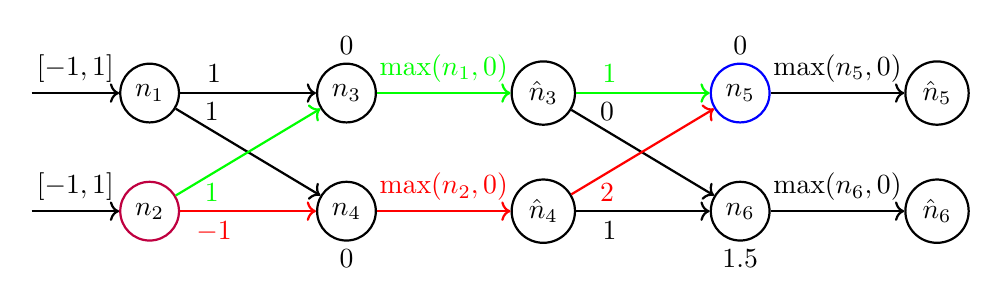
\begin{tikzpicture}
		
		\node[circle, draw= black, thick, minimum width = 20,
		minimum height = 20] (input1) {$n_1$};
		
		\node[circle, draw= purple, thick, minimum width = 20,
		minimum height = 20] (input2) at ($(input1) + (0,-1.5)$) {$n_2$};
		
		
		% Hidden layers
		
		\node (hidden10) at ($(input1) + (2.5,0.6)$) {$0$};
		
		\node (hidden20) at ($(input1) + (2.5,-1.5-0.6)$) {$0$};
		
		\node (hidden50) at ($(input1) + (7.5,0.6)$) {$0$};
		
		\node (hidden60) at ($(input1) + (7.5,-1.5-0.6)$) {$1.5$};
		
		
		\node[circle, draw= black, thick, minimum width = 20,
		minimum height = 20] (hidden1) at ($(input1) + (2.5,0)$) {$n_3$};
		\node[circle, draw= black, thick] (hidden2) at ($(input1) + (2.5,-1.5)$) {$n_4$};
		
		\node[circle, draw= black, thick, minimum width = 20,
		minimum height = 20] (hidden3) at ($(input1) + (5,0)$){$\hat{n}_3$};
		\node[circle, draw= black, thick] (hidden4) at ($(input1) + (5,-1.5)$) {$\hat{n}_4$};
		
		
		\node[circle, draw= blue, thick, minimum width = 20,
		minimum height = 20] (hidden5) at ($(input1) + (7.5,0)$){$n_5$};
		\node[circle, draw= black, thick] (hidden6) at ($(input1) + (7.5,-1.5)$) {$n_6$};
		
		
		
		
		% Output layer
		\node[circle, draw= black, thick, minimum width = 20,
		minimum height = 20] (output1) at ($(input1) + (10,0)$){$\hat{n}_5$};
		
		\node[circle, draw= black, thick, minimum width = 20,
		minimum height = 20] (output2) at ($(input1) + (10,-1.5)$){$\hat{n}_{6}$};
		
		
		% Connections
		
		\draw[->,thick] ($(input1) + (-1.5,0)$) -- (input1) node[midway, above] {$[-1,1]$};
		
		\draw[->,thick] ($(input1) + (-1.5,-1.5)$) -- (input2) node[midway, above] {$[-1,1]$};
		
		
		
		\draw[->,thick] (input1) -- (hidden1) node[near start, above] {$1$};
		\draw[->,thick] (input1) -- (hidden2)node[near start, above] {$1$};
		
		\draw[->,color=green, thick] (input2) -- (hidden1) node[near start, below] {$1$};
		\draw[->,color=red, thick] (input2) -- (hidden2)node[near start, below] {$-1$};
		
		
		
		
		
		\draw[->,color=green, thick] (hidden1) -- (hidden3) node[midway, above] {$\max(n_1,0)$};
		\draw[->,color=red, thick] (hidden2) -- (hidden4) node[midway, above] {$\max(n_2,0)$};
		
		
		
		
		
		\draw[->,color=green, thick] (hidden3) -- (hidden5) node[near start, above] {$1$};			
		\draw[->,thick] (hidden3) -- (hidden6) node[near start, above] {$0$};
		
		\draw[->,color=red, thick] (hidden4) -- (hidden5)node[near start, below] {$2$};
		\draw[->,thick] (hidden4) -- (hidden6)node[near start, below] {$1$};
		
		
		
		
		\draw[->,thick] (hidden5) -- (output1) node[midway, above] {$\max(n_5,0)$};
		\draw[->,thick] (hidden6) -- (output2) node[midway, above] {$\max(n_6,0)$};
		
		
	\end{tikzpicture}
	\caption{A DNN example from \cite{kpoly}: every neuron is separated into 2 nodes, $n$ pre- and $\hat{n}$ post-ReLU activation function. The pair $(n_2 n_3 n_5,n_2 n_4 n_5)$ in green and red is compensating (weights of paths are $1,-2$).}
	\label{fig1}
\end{figure}

The concept of value abstraction involves calculating upper and lower bounds for the values of certain neurons in a Deep Neural Network (DNN) when inputs fall within a specified range. This approach aims to assess the network's robustness without precisely computing the values for every input within that range.

Firstly, it's important to note that weighted sums represent a linear function, which can be explicitly expressed with relative ease. However, the ReLU (Rectified Linear Unit) function presents a challenge in terms of accurate representation. Although ReLU is a relatively straightforward piecewise linear function with two modes (one for $x<0$ and another for $x \geq 0$), it is not linear. The complexity arises when considering the compounded effects of the ReLU function across the various layers of a ReLU DNN. It's worth noting that representing $\ReLU(x)$ precisely is feasible when $x$ is "stable," meaning it's consistently positive or consistently negative, as there's only one linear mode involved in each scenario. Consequently, the primary challenge lies in addressing "unstable" neurons, where the linearity of the function does not hold consistently.


Consider the simpler abstraction, termed ``Box abstraction" \cite{deeppoly}: it inductively computes the bounds for each neuron in the subsequent layer independently. This is achieved by considering the weighted sum of the bounds from the previous layer, followed by clipping the lower bound at $\max(0,$ lower bound$)$ to represent the ReLU function, and so forth. For all $i$, define $x_i=\val_{\vx}(n_i)$, where $\vx=(x_1,x_2)$.

Taking the DNN example from Fig \ref{fig1}, assume $x_1,x_2 \in [-1,1]$. This implies that $x_3,x_4 \in [-2,2]$. After applying the ReLU function, $\hat{x}3,\hat{x}4$ are constrained to $[0,2]$, leading to $x_5 \in [0,6]$ and $x_6 \in [0,2]$. The bounds for $n_1, \ldots, n_4$ are exact, meaning for every $\alpha$ within the range, an input $\vy$ can be found such that $\val{\vy}(n_i)=\alpha$. However, this precision is lost from the next layer (beginning with $n_5, n_6$) due to potential dependencies among preceding neurons. For example, $n_3$ only attains the value $2$ when both $x_1$ and $x_2$ are $2$. In this case, $n_4$ would reach a value of $Val{(2,2)}(n_4)=0$. Consequently, it's implausible for $x_5=\Val_{\vx}(n_5)$ to reach $6$, as it would necessitate both $n_3$ and $n_4$ assuming the value $2$.

An extremely efficient algorithm that addresses some issues is "DeepPoly" \cite{deeppoly}, also independently discovered as the "CROWN" algorithm \cite{crown}. Instead of strict bounds, for each neuron $n$ in layer $k$, DeepPoly maintains two affine functions representing the lower and upper bounds of the neuron's value, based on inputs from the previous layer $k-1$. For instance, denote $f_i \leq x_i \leq g_i$ with, for example, $f_{3}(x_3)=f_4(x_4)=0$ and $g_3(x_3) = \frac{x_3+2}{2}$, $g_4(x_4) = \frac{x_4+2}{2}$. This leads to $x_5 \leq g_3(x_3) + 2 g_4(x_4) = \frac{x_3 + 2x_4 + 6}{2} = \frac{3x_1 - x_2 + 6}{2}\leq 5$.

For bounds $[\alpha,\beta]$ on $x_i$, the optimal linear function for the upper bound is $g_i(x_i)= \beta \frac{x_i-\alpha}{\beta-\alpha}$ for ReLU nodes. There are two options for the lower bound: $f^1_i(x_i) = 0$ or $f^2_i(x_i)=x_i$. DeepPoly selects between these based on the values of $\alpha$ and $\beta$ (for unstable neurons): if $|\alpha|\geq |\beta|$, then $f_i=f^1_i$ is chosen, otherwise, for $|\beta|>|\alpha|$, $f_i=f^2_i$ is selected. The variation, {\em $\overline{\mbox{DeepPoly}}$}, consistently chooses $f^1_i$, and never $f^2_i$. Contrary to DeepPoly, {\em $\overline{\mbox{DeepPoly}}$} encompasses the ``Box abstraction." For instance, with bounds $[-0.2,5]$ on $x_i$, it deduces $\ReLU(x_i) \in [0,5]$, whereas  DeepPoly without box abstraction algorithm would conclude $\ReLU(x_i) \in [-0.2,5]$.


\iffalse
\subsection{PRIMA and $\beta$-CROWN}
\fi

\subsection{MILP and LP encodings for DNNs}

At the other end of the spectrum, we find the Mixed Integer Linear Programming (MILP) value abstraction, which is a priori a complete method (albeit much slower than DeepPoly). 
Consider an unstable neuron $n \in[\alpha,\beta]$. The value $x$ of $\ReLU(n)$ can be encoded exactly in an MILP formula with one integer (actually even binary) variable $a$ valued in ${0,1}$, using 4 constraints \cite{MILP}:
\vspace{-0.1cm}
\begin{align*}
	\hat{x} \geq x \quad \wedge \quad \hat{x} \geq 0, \quad \wedge \quad \hat{x} \leq \beta \cdot a \quad \wedge \quad \hat{x} \leq x-\alpha \cdot (1-a)
\end{align*}

It can be shown that for all $x \in [\alpha,\beta] \setminus 0$, there exists a unique solution $(a,\hat{x})$ that meets these constraints, with $\hat{x}=\ReLU(x)$. Here, $a$ is 0 if $x < 0$, 1 if $x>0$, and can be either if $x=0$~\cite{MILP}. This encoding approach can be applied to every (unstable) ReLU node, and optimizing its value can help in certifying a given input. However, for networks with hundreds of nodes or more, the resulting MILP formulation will contain numerous integer variables and generally cannot be solved efficiently.

MILP instances can be linearly relaxed into LP over-abstraction, where variables originally restricted to integers in ${0,1}$ (binary) are relaxed to real numbers in the interval $[0,1]$, while maintaining the same encoding. As solving LP instances is polynomial time, this optimization is significantly more efficient. However, this efficiency comes at the cost of precision, often resulting in less stringent bounds. This approach is termed the {\em LP abstraction}

The following proposition shows that the LP abstraction refines the DeepPoly abstraction. 
The difference between the LP and the DeepPoly abstractions is that LP simultaneous considers the two linear lower bounding functions for the ReLU operation, namely $ReLU(x) \geq 0$ and $ReLU(x) \geq x$, while the DeepPoly abstraction restricts itself to the application of a single one of these linear bounding functions.
 

\begin{proposition}
	\label{LP}
	Given $x \in [\alpha,\beta]$ with $\alpha < 0 < \beta$, the following two systems of constraints 
	1) for LP and 2) for DeepPoly with both lower bounds are equivalent:
	\begin{align}
& \hat{x} \geq x \quad \wedge \quad \hat{x} \geq 0, \quad \wedge \quad \hat{x} \leq \beta \cdot a \quad \wedge \quad \hat{x} \leq x-\alpha \cdot (1-a), \, a \in [0,1]  \label{eq:lp}\\
&\hat{x} \geq x \quad \wedge \quad \hat{x} \geq 0 \quad \wedge \quad \hat{x} \leq \beta \frac{x-\alpha}{\beta-\alpha} \label{eq:deeppoly}
	\end{align} 
\end{proposition}

\begin{proof}
We need to show that the two upper bound constraints in Eq~\ref{eq:lp} is equivalent to the upper bound in Eq~\ref{eq:deeppoly}. To this end, we focus on the upper bound function in the linear variable $a \in  [0,1]$, with $x \in [\alpha,\beta]$ fixed. We have $\hat{x}$ in Eq~\ref{eq:lp} is upper bounded by $max_{a \in [0,1]} (min(\beta \cdot a, x - \alpha (1-a)))$, and this bound can be reached. Furthermore, 
	The function $\min(\beta \cdot a, x - \alpha (1-a))$ attains its maximum when $\beta \cdot a = x - \alpha (1-a)$, leading to the equation $(\beta - \alpha) a = x - \alpha$ and consequently $a = \frac{x - \alpha}{\beta-\alpha}$. This results in an upper bound of $\beta \cdot a = \beta \frac{x - \alpha}{\beta-\alpha}$ \qed
\end{proof}

\subsubsection*{Constraints for $\gamma$}

We could get the following constraints for $\gamma$, using $y_i$ and $\hat{y}_i$ to denote the $x_i-x_i'$ and $\hat{x}_i-\hat{x}_i'$:\begin{align*}
	\hat{y}_i \leq a \gamma_i \hspace*{2ex} &\wedge \hspace*{2ex}\hat{y} \geq y_i - a \gamma_i\\
	\hat{y}_i \geq (a-1) \gamma_i  \hspace*{2ex} &\wedge \hspace*{2ex} \hat{y} \leq y_i + (1-a) \gamma_i,
\end{align*} where $a$ is a binary variable, $\gamma_i$ is the upper bound of $x_i-x'_i$.


The following plot will show the above constraints:

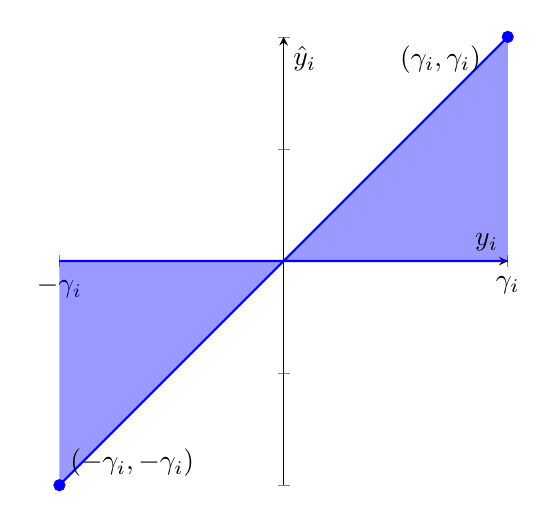
\begin{tikzpicture}
	\begin{axis}[
		xlabel={$y_i$},
		ylabel={$\hat{y}_i$},
		xmin=-2, xmax=2,
		ymin=-2, ymax=2,
		axis lines=center,
		samples=100, 
	 unit vector ratio=1 1 1, scale=1, xtick   = {-2,2},
	 xticklabels = {$-\gamma_i$,$\gamma_i$},
	 yticklabels = {},
		]
		\addplot[blue, thick, fill=blue, fill opacity=0.4] {x} \closedcycle; 
		\addplot[blue, thick] {0}; 
	
		\addplot[only marks, mark=*, mark size=2pt, blue] coordinates {(-2,-2)};
			\node[label={above:$(-\gamma_i,-\gamma_i)$}] at (axis cs: -1.35, -2.1) {};
			
				\addplot[only marks, mark=*, mark size=2pt, blue] coordinates {(2,2)};
			\node[label={above:$(\gamma_i,\gamma_i)$}] at (axis cs: 1.4, 1.5) {};
	\end{axis}
\end{tikzpicture}



The relation between $y_i$, $x'_i$ and $\hat{y}_i$ is $\hat{y}_i = \ReLU(x'_i+y_i)-\ReLU(x'_i).$ And its plots is as follows:

\hspace*{-10ex}
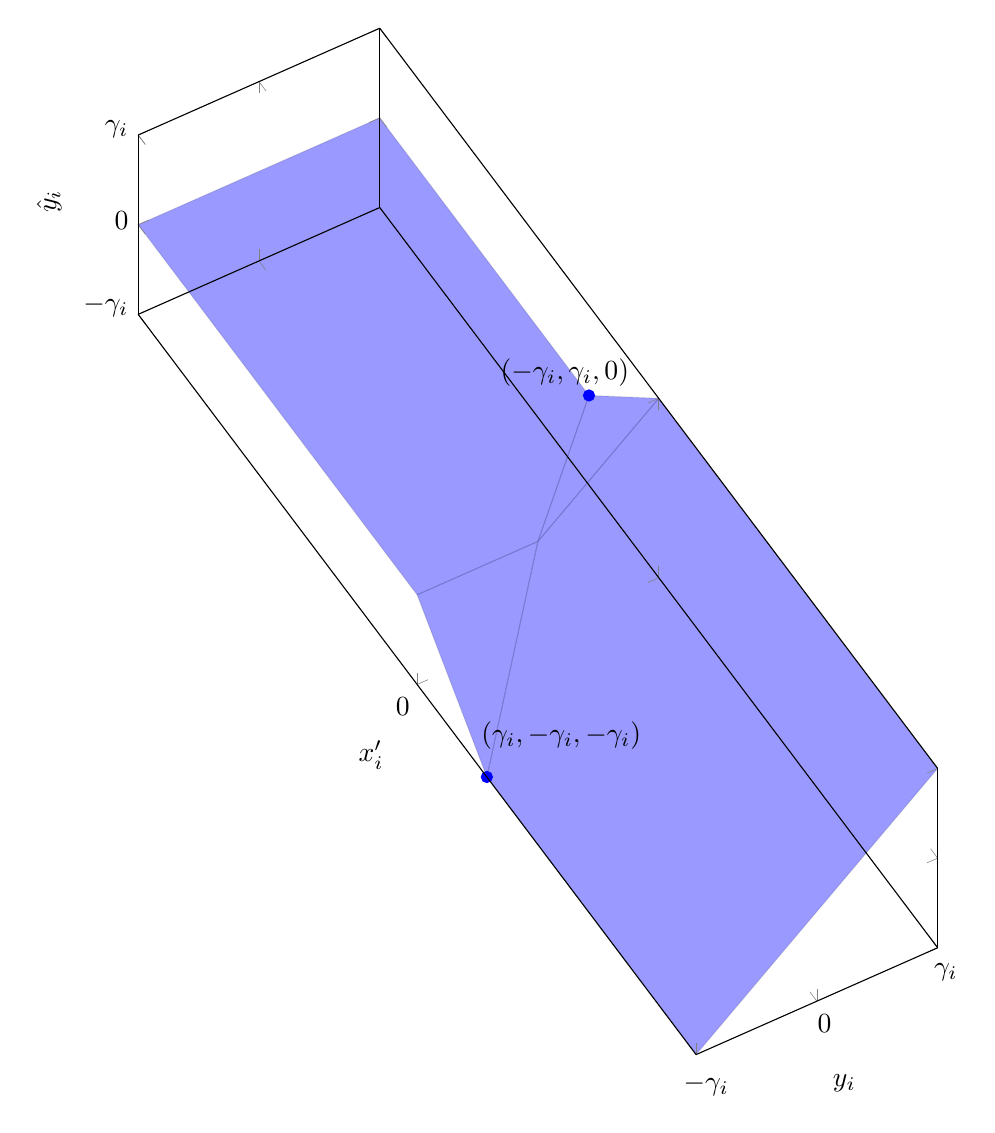
\begin{tikzpicture}
	\begin{axis}[	axis on top, xlabel = \(x'_i\),
		ylabel = {\(y_i\)}, zlabel = \(\hat{y}_i\),
				set layers=default,
	xmax = 4, xmin = -4,
ymax = 1, ymin = -1,		
zmax = 1, zmin = -1,
				unit vector ratio=1 1 1, scale=3,
				view={60}{50}, ytick   = {-1,0,1},
				yticklabels = {$-\gamma_i$,$0$,$\gamma_i$}, xtick = {0},
				xticklabels = {$0$}, ztick   = {-1,0,1},
				zticklabels = {$-\gamma_i$,$0$,$\gamma_i$},
				]
		\addplot3[fill=blue,opacity=0.1, fill opacity=0.4] 
		coordinates {
	 (0,0,0) (-1,1,0) (-4,1,0) (-4,-1,0) (0,-1,0) (0,0,0)
		};
		
		\addplot3[fill=blue,opacity=0.1, fill opacity=0.4	] 
		coordinates { (0,0,0) (0,1,1) (4, 1, 1) (4, -1, -1) (1,-1,-1) (0,0,0)
		};
		
		\addplot3[fill=blue,opacity=0.1, fill opacity=0.4	] 
		coordinates { (0,0,0)  (-1,1,0) (0,1,1) (0,0,0)
		};
		
			\addplot3[fill=blue,opacity=0.1, fill opacity=0.4	] 
		coordinates { (0,0,0)  (0,-1,0) (1,-1,-1) (0,0,0)
		};
		
		\addplot3[only marks, mark=*, mark size=2pt, blue] coordinates {(1,-1,-1)};
					\node[label={$(\gamma_i,-\gamma_i, -\gamma_i)$}] at (axis cs: 1.2, -0.5 ,-1) {};
					
			\addplot3[only marks, mark=*, mark size=2pt, blue] coordinates {(-1,1,0)};
		\node[label={$(-\gamma_i,\gamma_i, 0)$}] at (axis cs: -1, 0.8 ,0) {};			
		
	\end{axis}
\end{tikzpicture}



\hspace*{-15ex}
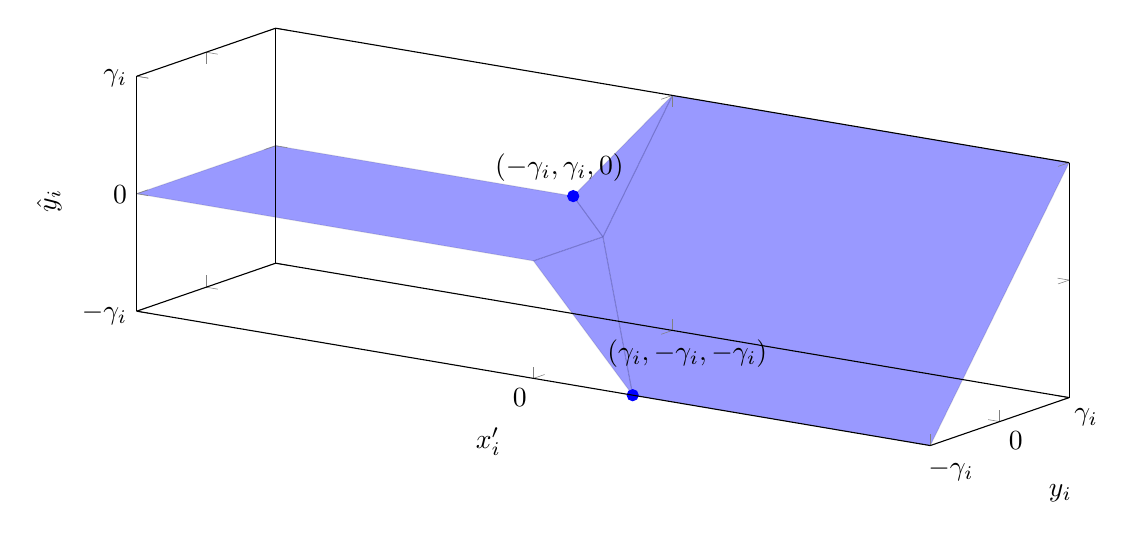
\begin{tikzpicture}
	\begin{axis}[	axis on top, xlabel = \(x'_i\),
		ylabel = {\(y_i\)}, zlabel = \(\hat{y}_i\),
		set layers=default,
				xmax = 4, xmin = -4,
		ymax = 1, ymin = -1,		
				zmax = 1, zmin = -1,
		unit vector ratio=1 1 1, scale=2.5,  ytick   = {-1,0,1},
		yticklabels = {$-\gamma_i$,$0$,$\gamma_i$}, xtick = {0},
		xticklabels = {$0$}, ztick   = {-1,0,1},
		zticklabels = {$-\gamma_i$,$0$,$\gamma_i$},
		view={35}{14},
		]
		\addplot3[ fill=blue,opacity=0.1, fill opacity=0.4] 
		coordinates {
			(0,0,0) (-1,1,0) (-4,1,0) (-4,-1,0) (0,-1,0) (0,0,0)
		};
		
		\addplot3[	fill=blue,opacity=0.1, fill opacity=0.4] 
		coordinates { (0,0,0) (0,1,1) (4, 1, 1) (4, -1, -1) (1,-1,-1) (0,0,0)
		};
		
		\addplot3[	fill=blue,opacity=0.1, fill opacity=0.4	] 
		coordinates { (0,0,0)  (-1,1,0) (0,1,1) (0,0,0)
		};
		
		\addplot3[	fill=blue,opacity=0.1, fill opacity=0.4	] 
		coordinates { (0,0,0)  (0,-1,0) (1,-1,-1) (0,0,0)
		};
		
			\addplot3[only marks, mark=*, mark size=2pt, blue] coordinates {(1,-1,-1)};
		\node[label={$(\gamma_i,-\gamma_i, -\gamma_i)$}] at (axis cs: 1.2, -0.5 ,-1) {};
		
		\addplot3[only marks, mark=*, mark size=2pt, blue] coordinates {(-1,1,0)};
		\node[label={$(-\gamma_i,\gamma_i, 0)$}] at (axis cs: -1, 0.8 ,0) {};			
		
	\end{axis}
\end{tikzpicture}


%\begin{tikzpicture}[
%	declare function={
%		f(\x,\y)=max((\x+\y),0)-max(\x,0);
%	}]
%	\begin{axis}[axis lines=center,
%		axis on top,
%		set layers=default,
%		xrange=-3:3,
%		yrange=-2:2,
%		unit vector ratio=1 1 1,% <- HERE (taken from Phelype Oleinik's deleted answer)
%		scale=3 %<- added to compensate for the downscaling
%		% resulting from unit vector ratio=1 1 1
%		]
%		\addplot3[
%		domain=-3:3,
%		domain y=-1:1, surf,
%		samples=40,
%		samples y=40,
%		] {f(\x,\y)};
%	\end{axis}
%\end{tikzpicture}





\section{Compensating pairs of paths}
\label{Sec.comp}

In this section, we explore the key factor for the loss of accuracy in value 
abstraction methodologies. To this end, we first introduce the novel notion of compensating paths:

\begin{definition}
A pair $(\pi,\pi')$ of paths is {\em compensating} if:
\begin{itemize}
	\item they have the same starting node $a$ (called {\em source} state) and ending node $b$ (called {\em target} state of $(\pi,\pi')$),
	\item they are disjoints (the only common nodes are the source and the target),
	\item the weights satisfy $weight(\pi') < 0 < weight(\pi)$.
\end{itemize}	
We call a path $\pi$ {\em compensating} if there exists a path $\pi'$ such that either $(\pi,\pi')$ or $(\pi',\pi)$ is compensating.
\end{definition}

\begin{example}
	For instance, on Fig.~\ref{fig1}, the paths $\pi= n_2 n_3 n_5$ has weight $1$, while the
	path $\pi'= n_2 n_4 n_5$ has weight $-2$, hence $(\pi,\pi')$ is a compensating pair of paths.
	\end{example}


The phenomenon of compensating pairs of paths significantly impacts the precision of the target state due to the overabstraction of values. For instance, consider a scenario where $x_5 \leq 4$ is attainable when $x_1=1$ and $x_2=-1$, leading to $\val_{(1,-1)}(n_5)=4$. However, the Box methodology estimates an upper limit of $6$. Although DeepPoly partially rectifies the dependency on $x_2$, it achieves only partial negation of the $x_2$ value owing to the excessive abstraction characteristic of ReLU. This results in an overestimated upper bound of $x_5 \leq 5$ through a contribution of $\frac{-x_2+3}{2} \leq 2$, as opposed to the exact calculation of $-x_2 \leq 1$, culminating in a precise upper bound of $x_5 \leq 4$.

In an intuitive sense, the target state accrues weight from the source state via different paths connecting the source to the target. When these connecting paths possess weights of contrasting signs, a certain degree of cancellation occurs, with the extent of cancellation being up to $min(|weight(\pi')|,|weight(\pi')|)$. This mechanism also serves to mitigate error propagation in a manner similar to how $0 = |1+(-1)| \leq |1|+|-1| = 2$ in imprecise analyses. However, the ReLU functions can constrain the level of compensation due to their clipping effect. For instance, if the inputs $x_1, x_2$ are confined within the range $[-1,-0]$, then $\hat{x}_3$ will consistently be 0 for any input $\vx=(x_1,x_2)$ within the domain $[-1,-0] \times [-1,-0]$, thereby preventing $weight(\pi')$ from effectively counterbalancing $weight(\pi')$.




\iffalse
\vspace*{2ex}

\begin{figure}
	\centering
	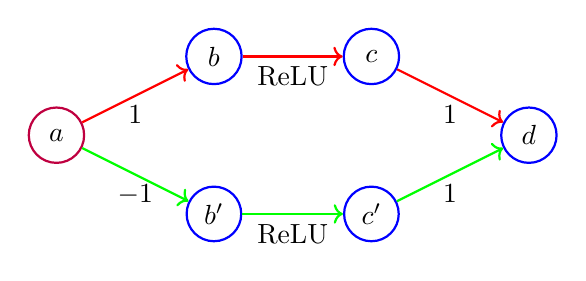
\begin{tikzpicture}
		
		\node[circle, draw= purple, thick, minimum width = 20,
		minimum height = 20] (input1) {$a$};
		
		
		% Hidden layers
		\node[circle, draw= blue, thick, minimum width = 20,
		minimum height = 20] (hidden1) at ($(input1) + (2,1)$) {$b$};
		\node[circle, draw= blue, thick] (hidden2) at ($(input1) + (2,-1)$) {$b'$};
		
		\node[circle, draw= blue, thick, minimum width = 20,
		minimum height = 20] (hidden3) at ($(input1) + (4,1)$){$c$};
		\node[circle, draw= blue, thick] (hidden4) at ($(input1) + (4,-1)$) {$c'$};
		
		% Output layer
		\node[circle, draw= blue, thick, minimum width = 20,
		minimum height = 20] (output) at ($(input1) + (6,0)$){$d$};
		
		% Connections
		\draw[->,thick,draw= red] (input1) -- (hidden1) node[midway, below] {$1$};
		\draw[->,thick,draw= green] (input1) -- (hidden2)node[midway, below] {$-1$};
		
		\draw[->,thick,draw= red] (hidden1) -- (hidden3) node[midway, below] {$\ReLU$};
		\draw[->,thick,draw= green] (hidden2) -- (hidden4) node[midway, below] {$\ReLU$};
		
		\draw[->,thick,draw= red] (hidden3) -- (output)node[midway, below] {$1$};
		\draw[->,thick,draw= green] (hidden4) -- (output)node[midway, below] {$1$};
	\end{tikzpicture}
\end{figure}

\vspace*{2ex}

In this figure, $a$ is the input neuron; $bc,b'c'$ are nodes in the hidden layer, ($b,b'$ are pre-activation and $c,c'$ are post activation); and $d$ is the unique output neuron. The numbers next to the arrows are the weights. So, $W_{ba}=1$ and $W_{b'a}=-1$, $W_{dc}=W_{dc'}=1$. The pair of these two paths, $a$ to $bc$ to $d$, and $a$ to $b'c'$ to $d$, is a so called \emph{Compensating Pair}. Because its shape looks like a diamond, it is also called a Diamond. The characteristic is that, the products of all weights in the paths, have two different signs: along $bc$, the product is (strictly) positive, while along $b'c'$, the product is (strictly) negative. 

The existence of compensating pairs is key reason why simple approximation like LP or Interval Arithmetic cannot get the exact upper and lower bounds. If both pairs are negative or positive, LP or even Interval Arithmetic will get the exact values of lower and upper bounds.


To explain why, suppose we have another input node $a'$, such that both $a$ and $a'$ has an input interval $[0,1]$, but the weight from $a'$ to $b$ or $b'$ are both $1$. Then both $b$ will have an interval $[0,2]$ and $b'$ will have an interval $[-1,1]$. More importantly, in LP formulation, $c$ will be $b$ but $c'$ will be $0.5(b')+0.5$. The upper bound of $d$ will be $c+c'$, and hence $b+0.5(b')+0.5$, and hence $a+a'+0.5a'-0.5a'+0.5=0.5a+1.5a'+0.5$. And this will leads to a upper bound $2.5$ but this is not exact.

\vspace*{2ex}
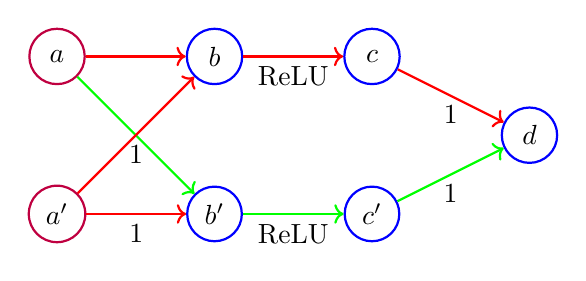
\begin{tikzpicture}
	\node[circle, draw= purple, thick, minimum width = 20,
	minimum height = 20] (input1) {$a$};
	
	\node[circle, draw= purple, thick, minimum width = 20,
	minimum height = 20] (input2) at ($(input1) + (0,-2)$) {$a'$};
	
	
	% Hidden layers
	\node[circle, draw= blue, thick, minimum width = 20,
	minimum height = 20] (hidden1) at ($(input1) + (2,0)$) {$b$};
	\node[circle, draw= blue, thick] (hidden2) at ($(input1) + (2,-2)$) {$b'$};
	
	\node[circle, draw= blue, thick, minimum width = 20,
	minimum height = 20] (hidden3) at ($(input1) + (4,0)$){$c$};
	\node[circle, draw= blue, thick] (hidden4) at ($(input1) + (4,-2)$) {$c'$};
	
	% Output layer
	\node[circle, draw= blue, thick, minimum width = 20,
	minimum height = 20] (output) at ($(input1) + (6,-1)$){$d$};
	
	% Connections
	\draw[->,thick,draw= red] (input1) -- (hidden1);
	\draw[->,thick,draw= green] (input1) -- (hidden2);
	
	\draw[->,thick,draw= red] (input2) -- (hidden1) node[midway, below] {$1$};
	\draw[->,thick,draw= red] (input2) -- (hidden2)node[midway, below] {$1$};
	
	\draw[->,thick,draw= red] (hidden1) -- (hidden3) node[midway, below] {$\ReLU$};
	\draw[->,thick,draw= green] (hidden2) -- (hidden4) node[midway, below] {$\ReLU$};
	
	\draw[->,thick,draw= red] (hidden3) -- (output)node[midway, below] {$1$};
	\draw[->,thick,draw= green] (hidden4) -- (output)node[midway, below] {$1$};
\end{tikzpicture}
\vspace*{2ex}

The general formal definition of compensating pair is as follows:

\begin{definition} In a full-connected network with $\ReLU$ as activation function:
	
	1. A path is a sequence of nodes $\langle a,b,c,d,e,\cdots\rangle$ of nodes that goes consecutively through each layer. We call the first node source node and the last node target node.  
	
	2. The \emph{Value} of a path is the product of of weights along the path (with sign): for a path $\langle a,b,c,d,e,\cdots\rangle$, its values is $$V = W_{ab}\cdot W_{bc}\cdot W_{cd}\cdot W_{ed}\cdot \cdots$$
	
	3. A \emph{Compensating Pair} is a pair of paths with the same source node and target node, such that the two paths have no common node, and the values of two paths have opposite signs (one is strictly positive and another is strictly negative).
	
	We also use \emph{Diamond} to call a compensating pair in the network.
\end{definition}

The following theorem shows the role of compensating pairs in the computation:

\fi

\begin{table}[b!]
	\centering
	\begin{tabular}{|c|c|c|c|}
		\hline
		\text{Source/Target Layers}  &  \text{Natural DNN} & \text{Robust DNN} & \text{Ratio Natural vs Robust} \\ \hline \hline
		0 / 2 & 0.0304 & 0.00220  & 13.8x\\ \hline
		1 / 3  & 0.0313 & 0.00875 & 3.58x \\ \hline
		2 / 4  &  0.0267 & 0.00785 & 3.40x \\ \hline
		3 / 5  &  0.0253 & 0.00804  & 3.18x \\ \hline
	\end{tabular}
	\caption{Comparison of the average compensation strength over all the pairs of nodes of layer source/target between a DNN naturally-trained and a DNN robustly-trained using DiffAI \cite{DiffAI} with the same architecture and training set. {\color{red} Compensating strength with 1 layer between source and target is straightforward, and was sufficient to show the difference between DNNs trained naturally and by DiffAI.}}
	\label{tab:compensation}
\end{table}


The discussion so far shows  that compensation is one of the possible factors contributing to inaccuracy. We now establish that it is the sole cause of inaccuracy:
if a DNN lacks any compensating path, then any methodology that is at least as accurate as the Box abstraction, such as LP and $\overline{\mbox{DeepPoly}}$ (but not DeepPoly), will precisely determine the exact upper and lower bounds for every node. This assertion is formalized in the following theorem:

\begin{theorem}
	\label{th1}
	Consider any node $n$ within a DNN devoid of any compensating path. Let $[\alpha,\beta]$ represent the bounds computed by the Box abstraction for node $n$. Then, for every $\gamma$ within the interval $[\alpha,\beta]$, there exists an input $\vx$ such that $\val_{\vx}(n) = \gamma$.
\end{theorem}

The sketch of proof can be found in Section \ref{sec.proofs}. 

This theorem underscores the significant role of compensating paths in the accuracy of bound estimation within DNNs, affirming that their absence guarantees the precision of computed bounds. Practically speaking, encountering a network entirely devoid of compensating paths is highly improbable, rendering this more a theoretical observation, highlighting that compensation is a key driver of inaccuracy.




%It is worth remarking that  Theorem~\ref{th1} does not directly apply to standard DeepPoly since DeepPoly does not inherently refine the Box abstraction.  Furthermore, it is unclear whether  Theorem~\ref{th1} applies to PRIMA or $\beta$-CROWN as these techniques refine DeepPoly.  Nevertheless, this limitation could potentially be addressed by integrating $\overline{\text{DeepPoly}}$.

An intriguing application of this result lies in elucidating why certain DNNs are inherently more amenable to verification compared to others. This distinction is notably evident between DNNs adversarially trained for robustness and those trained naturally, utilizing the same architecture \cite{deeppoly,prima,crown}. Notably, the presence of compensating pairs is an intrinsic structural attribute of the learned DNN, contrasting with more semantic aspects like the number of unstable ReLUs, which are significantly influenced by the specific image and algorithm employed. To illustrate this point, we consider two networks, each comprising 5 hidden layers with 100 nodes, sourced from the ERAN GitHub repository. One is naturally trained ($6\times100$), and the other is trained using DiffAI ($5\times100$). In Table \ref{tab:compensation}, we present the average compensation strength, computed as the mean of $max_{\pi,\pi'} min(|weight(\pi')|,|weight(\pi')|)$ across all source/target states within specified layers. The findings reveal that the average compensation strength is considerably lower in the Robust DNN compared to the natural DNN. Correspondingly, the Robust DNN is substantially easier to verify than its natural counterpart, as evidenced by the enhanced accuracy and image verification rate of DeepPoly.


\subsection{MILP$_{X_n}$}



While Theorem \ref{th1} is interesting to understand that compensation is a key notion for accurate verification of DNNs, it cannot be used directly to analyze DNNs with compensations, which are actually those that are most interesting to tackle.
Intuitively, when there are compensating paths, it seems necessary to consider exactly the (unstable) ReLU nodes that are seen along these paths. 
%Consider a neuron $n$ in layer $k$ for which we want to have accurate bounds 
%$[\alpha,\beta]$.

Consider a neuron $n$ in layer $k$, for which we aim to establish accurate bounds $[\alpha,\beta]$. Define $X_n$ as the set of neurons $x$ in layers up to $k-1$, where each $x$ is part of a compensating path targeting neuron $n$, but not as the source or the target node of the path. Let $Y_n$ represents the set of all other neurons in the first $k-1$ layers, essentially serving as the complement of $X_n$. We introduce MILP${X_n}$, a variant of the MILP encoding where all nodes in $Y_n$ are linearly relaxed, hence incorporating $|X_n|$ binary variables, each corresponding to a neuron in $X_n$. Additionally, this encoding encapsulates bounds for every neuron $n'$ in the initial $k-1$ layers, as computed inductively in previous steps. That is, we do not use explicitly in $X_n$ nodes on compensating paths with target neurons before $n$ ({\em indirectly} compensating paths), 
only those with target $n$ ({directly} compensating paths).
The contribution of these {\em indirectly} compensating paths are thus 
only taken into account indirectly via the bounds on previous neurons computed inductively,
and not as binary variables. We demonstrate now that the bounds $[\alpha,\beta]$ for neuron $n$, as computed by MILP${X_n}$, are accurate, thereby offering a more nuanced approach to DNN verification in scenarios involving compensating paths.
We will provide the proof under a fairly light well-connected hypothesis (H1), which only DNNs where all but very few weights are 0 does not satisfy.

(H1): for every 2 (not necessarily disjoint) paths $\rho_1,\rho_2$ with non-zero weight with the same source $m$ and the same target $n$ with at least 2 transitions, there exists another path $\rho_3$ from $m$ to $n$ (with non zero-weight) totally disjoint from $\rho_1$ and $\rho_2$ (except at the source and target). This hypothesis is used to remove corner cases which will not happen in actual DNNs, which all are well-connected.


\begin{theorem}
	\label{th2} 
	Assume the DNN satisfies the well-connected (H1) hypothesis.
	Let $n$ be any node of a DNN. Then for $[\alpha,\beta]$ the bounds computed by MILP$_{X_n}$ for neuron $n$, for all $\gamma \in [\alpha,\beta]$, there exists an input $\vy$ such that $\val_{\vy}(n)=\gamma$.
\end{theorem}

The sketch of proof of Theorem \ref{th2} can be found in Section \ref{sec.proofs2}.


\subsection{Sketch of Proof for Theorem \ref{th1}}
\label{sec.proofs}

First, notice that by continuity of all the functions used in the DNNs, it suffices to show both theorem for $\gamma=\alpha$ and $\gamma=\beta$.

%Intuitively, our first proof shows that if there are no compensation, then there are no correlations between nodes.
Consider a target neuron $z$.
In case there is no compensating path, we can assign a sign to each neuron $n$: 0
if all paths from $n$ to $z$ has weight 0, $+1$ if all paths have positive weights, and 
$-1$ if they have negative weights. 

Using the concept of sign, we introduce input vectors $\vx^{*}, \vx^{\sharp}$: 

\begin{definition}
We define the following two input vectors $\vx^{*}, \vx^{\sharp}$ in $\cal B$: 
	\begin{itemize}
		\item $\vx^{*}$ is the input vector defined in the following way:
		\begin {itemize}
		 \item $x^*_{a_i}=\max(a_i)$ if $S(a_i)\in \{0,1\}$, and
          \item $x^*_{a_i}=\min(a_i)$ otherwise, that is when $S(a_i)=-1$.
	\end{itemize}
		
		\item $\vx^{\sharp}$ is the input vector defined in the following way:
		\begin{itemize}
			\item $x^{\sharp}_{a_i}=\min(a_i)$ if $S(a_i)\in \{0,1\}$, and
			\item $x^{\sharp}_{a_i}=\max(a_i)$ otherwise, that is when $S(a_i)=-1$.
		\end{itemize}
	\end{itemize}
\end{definition}



We can then prove that $\vx^\star,\vx^\sharp$ maximize and minimize conjointly all the nodes in the DNN. Notice that it does {\em not} mean that there is no dependencies between nodes.
There can be correlations between nodes, just they do not affect the $\min$ and $\max$ bounds that can be reached in any node.

\begin{proposition}
	\label{prop.sign}
	${\vx^\star}$ maximizes the value of all positive neurons and minimizes the value of all negative neurons, and  
	${\vx^\sharp}$ minimizes the value of all positive neurons and maximizes the value of all negative neurons.
\end{proposition}

Hence $\val_{\vx^\star}(z)=\beta$ and $\val_{\vx^\sharp}(z)=\alpha$,
for $[\alpha, \beta]$ the bounds computed by the Box abstraction. We conclude Theorem \ref{th1} by invocking continuity.

\smallskip
The formal proof is in appendix A.


\subsection{Sketch of Proof for Theorem \ref{th2}}
\label{sec.proofs2}

\begin{figure}[h]
	\centering
	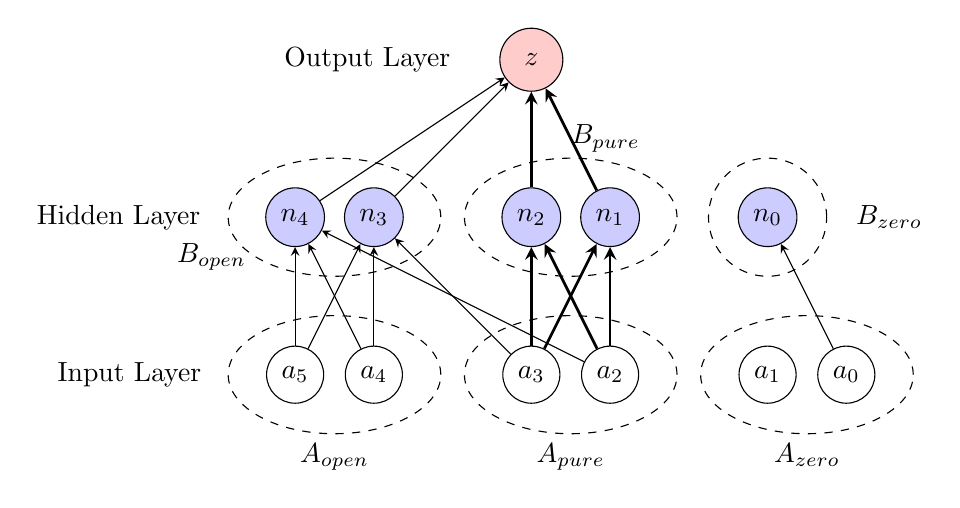
\begin{tikzpicture}[>=stealth, node distance=2cm]
		% Input nodes (two types)
		\node[circle, draw, minimum size=0.5cm] (input1) at (-1,0) {$a_0$};
		\node[circle, draw, minimum size=0.5cm] (input2) at (-2,0) {$a_1$};
		\node[circle, draw, minimum size=0.5cm] (input3) at (-4,0) {$a_2$};
		
		\node[circle, draw, minimum size=0.5cm] (input4) at (-5,0) {$a_3$};
		\node[circle, draw, minimum size=0.5cm] (input5) at (-7,0) {$a_4$};
		\node[circle, draw, minimum size=0.5cm] (input6) at (-8,0) {$a_5$};
	
		\draw[draw=black, dashed] (-1.5,0) ellipse (1.35 and 0.75);
		\node[below] at (-1.5,-0.75) {$A_{zero}$};
		
		\draw[draw=black, dashed] (-2,2) ellipse (0.75 and 0.75);
		\node[right] at (-1,2) {$B_{zero}$};
		
		% Hidden layer nodes
		
		\node[circle, draw, minimum size=0.5cm, fill=blue!20] (hidden1) at (-2,2) {$n_0$};
		
		\node[circle, draw, minimum size=0.5cm, fill=blue!20] (hidden2) at (-4,2) {$n_1$};
		\node[circle, draw, minimum size=0.5cm, fill=blue!20] (hidden3) at (-5,2) {$n_2$};
		
		\node[circle, draw, minimum size=0.5cm, fill=blue!20] (hidden4) at (-7,2) {$n_3$};
		\node[circle, draw, minimum size=0.5cm, fill=blue!20] (hidden5) at (-8,2) {$n_4$};
		
		
		
		\draw[draw=black, dashed] (-4.5,0) ellipse (1.35 and 0.75);
		\node[below] at (-4.5,-0.75) {$A_{pure}$};
		
		
		\draw[draw=black, dashed] (-7.5,0) ellipse (1.35 and 0.75);
		\node[below] at (-7.5,-0.75) {$A_{open}$};
		
		
		
		\draw[draw=black, dashed] (-4.5,2) ellipse (1.35 and 0.75);
		\node[left] at (-3.5,3) {$B_{pure}$};
		
		
		\draw[draw=black, dashed] (-7.5,2) ellipse (1.35 and 0.75);
		\node[left] at (-8.5,1.5) {$B_{open}$};
		
		
		
		% Output node
		\node[circle, draw, minimum size=0.8cm, fill=red!20] (output) at (-5,4) {$z$};
		
		
		% connections
		
		\draw[->] (input1) -- (hidden1);
		
		\draw[->] (input3) -- (hidden5);
		
		\draw[->] (input4) -- (hidden4);
		
		
%		% Connect input to hidden layer
		\foreach \i in {3,4} {
			\foreach \h in {3,2} {
				\draw[line width=1pt, ->] (input\i) -- (hidden\h);
			}
		}
		
		
		\foreach \i in {5,6} {
			\foreach \h in {4,5} {
				\draw[->] (input\i) -- (hidden\h);
			}
		}
%		
		% Connect hidden layer to output
		\foreach \h in {2,3} {
			\draw[line width=1pt,->] (hidden\h) -- (output);
		}
		
		\foreach \h in {4,5} {
			\draw[->] (hidden\h) -- (output);
		}
		
%\		% Input label
		\node[left=0.7cm of input6] {Input Layer};
		
		% Hidden label
		\node[left=0.7cm of hidden5] {Hidden Layer};
	
		% Output label
		\node[left=0.5cm of output] {Output Layer};
	\end{tikzpicture}
	\caption{Definitions in the proof of Theorem \ref{th2}}
	\label{fig:neural_network_types_simplified}
\end{figure}

Concerning Theorem \ref{th2}, consider an output node $z$.
Let $[\alpha(z),\beta(z)]$ be the bound computed by $\MILP_{X_z}$.
%We will show the existence of $\vx^\sharp,\vx^\star$
%such that $\val_{\vx^\sharp}(z)=\alpha$ and $\val_{\vx^\star}(z)=\beta$,
%and we will get the proof of Theorem 2 by a continuity argument.
%For that, 
We partition the input neurons from layer $0$ into:
\begin{enumerate}
	\item $A_{zero}= \{a \mid \forall \text{ path $\rho$ from $a$ to } z, weight(\rho)=0\}$.
	\item $A_{pos}= \{a \mid \forall \text{ path $\rho$ from $a$ to } z, weight(\rho)\geq0\}$.
	\item  $A_{neg}= \{a \mid \forall \text{ path $\rho$ from $a$ to } z, weight(\rho)\leq0\}$.
	Let $A_{pure}=A_{pos} \cup A_{neg}$.
	\item $A_{open}$ is the set of remaining input neurons.
\end{enumerate}

We then partition the set of neurons in hidden layers: 
\begin{enumerate}
	\item $B_{zero}= \{n \mid \forall \text{ path $\rho$ from $n$ to } z, weight(\rho)=0\}$.
	\item $B_{open}$ is the set of neurones reachable with $>0$ weight from $A_{open}$ and such that there is at least one path to $z$ with non zero weight.
	\item $B_{pure}$ is the set of remaining neurons.
\end{enumerate}

We can show the following lemma:

\begin{lemma}
	$A_{pure} \cup B_{pure} $ forms a sub-network, denoted $D_I$. That is, 
	for $n \in B_{pure}$, for every path $\rho$ from $m$ to $n$
	either $m \in B_{pure}\cup I$ or $weight(\rho)=0$.
\end{lemma}

Hence, the value of any neuron $n$ in $A_{pure}$ or $B_{pure}$ is entirely determined by 
inputs in $A_{pure}$. 


We cannot define the Sign function on nodes from which a compensating path can be reached.
However, we can define the sign function for neurons in $A_{pure}$ and $B_{pure}$.
Further, the set of nodes on which the sign function is defined is suffix-closed:

\begin{lemma}
	Let $m,n$ be two nodes, such that $S$ is defined on $m$ and there is a path $\rho$ with non zero weight to a node $n$. Then $S$ is defined on $n$.
	Further, $S(n)= Sign(weight(\rho)) S(m)$.
\end{lemma}

We can apply Theorem \ref{th1} on the DNN made of nodes from $A_{pure}$ and $B_{pure}$, and obtain $\vx_{pure}^\star,\vx_{pure}^\sharp$ optimizing neurons in $A_{pure}$ or $B_{pure}$:

\begin{proposition}
For a node $b$ with $S(b)=1$:

$$\max(b)=\max_{\vx_{open}} \val_{\vx^{\star}_{pure},\vx_{open}}(b)$$
$$\min(b)=\min_{\vx_{open}} \val_{\vx^{\sharp}_{pure},\vx_{open}}(b)$$

and for $S(b)=-1$:
$$\max(b)=\max_{\vx_{open}} \val_{\vx^{\sharp}_{pure},\vx_{open}}(b)$$
$$\min(b)=\min_{\vx_{open}} \val_{\vx^{\star}_{pure},\vx_{open}}(b)$$
\end{proposition}

Consider the DNN $D'$ with input nodes $A_{open}$, where all the 
edges from $m \in A_{open} \cup B_{open}$ to $n$ are replaced by a bias 
(equals to the weight of the edge times the fix value $\val_{\boldsymbol{x}^\star_{open}}(m)$) for $n$ (we sum all these bias for a neuron $n$).
The values in $D'$ are the same as the values in $D$ for input $\vx^{\star}_{pure}$,
which suffices to reach the maximal value of $D$.
In $D'$, all the ReLU nodes are in $B_{open}$. 
Hence $\MILP_{B_{open}}$ computes the bounds accurately in $D'$.
It will compute the bound in the same way in $D$, hence we get $\beta=\max(z)$ for the target $z$. The formal proof is in appendix B.


\subsection{An efficient algorithm}


Leveraging Theorem \ref{th2}, it is theoretically feasible to procure accurate bounds by iteratively applying MILP$_{X}$ to each node, layer by layer. This sequential approach would yield precise bounds $[\alpha,\beta]$ for each node, which could then be utilized to calculate accurate bounds for subsequent layers. However, in a practical setting, this methodology may prove to be computationally inefficient. Typically, the set $X_n$ includes a substantial portion of the nodes from all preceding layers up to layer $k-1$ for a given node $n$ in layer $k$. Instead, an interesting trade off between speed and accuracy is to set a threshold on the strength of compensation. Paths falling below this threshold are deemed to not warrant an individual integer variable due to insufficient compensatory strength. We denote the resultant subset of nodes situated on paths with substantial compensation as $Z_n$. In practical applications, one might consider selecting the $K$ nodes that are involved in the most significant compensating paths to construct the set $Z_n$, with $K$ being a relatively small integer. This strategy effectively provides a trade-off between the algorithm's performance and the precision of the results. The detailed steps of this approach are outlined in the pseudo-code for \CMP presented in Algorithm \ref{algo1}.





\SetKwInput{KwInput}{Input}
\SetKwInput{KwOutput}{Output}

\begin{algorithm}[b!]
	\caption{CMP($K$)}
	\label{algo1}
	\KwInput{Bounds $[\alpha_n,\beta_n]$ for input nodes $n$ at layer $0$ (input neighbourhood)}
	
	\KwOutput{Bounds $[\alpha_n,\beta_n]$ for every node $n$}
	
	\For{layer $k=1 \cdots \ell$}{
		\For{neuron $n$ in layer $k$}{
			
			Compute $Z$ a set of $K$ nodes covering the compensating pairs of paths with target $n$
			with heaviest compensation
			
			Run MILP$_Z$ to obtain $[\alpha_n,\beta_n]$ from bounds of neurons in layers $< k$
		}
	}
\end{algorithm}	




CMP($K$) has a worst case complexity bounded by $O(N \MILP(N,K))$, 
where $N$ is the number of nodes of the DNN, 
and $\MILP(N,K)$ is the complexity of solving a MILP program with $K$ integer variables and $N$ linear variables.
We have $\MILP(N,K) \leq 2^K \LP(N)$ where $\LP(N)$ is the Polynomial time to solve a Linear Program with $N$ variables.

Notably, this complexity serves as an upper bound. For instance, solvers like Gurobi are quite adept and usually do not need to evaluate all $2^K$ ReLU configurations to deduce the bounds.
It's worth mentioning that the for loop iterating over neurons $n$ in layer $k$, as seen in line 2, can be executed in parallel. This is feasible because the computation only depends on bounds from preceding layers, not the current layer $k$. This parallelization results in a time complexity of $O(\sum_{i=1}^{\ell} \MILP(N_{i-1},K))$, where $\ell$ denotes the total number of layers and $N_i$ the count of neurons in layers $0, ..., i$.


Therefore, if $K$ is sufficiently small, Algorithm \ref{algo1} frequently invokes MILP (e.g., using Gurobi) with a manageable number of integer variables. This approach is expected to be efficient and yet remains fairly precise, as it can accurately compute (according to Theorem \ref{th2}) the most significant compensating path. The effectiveness of this strategy is further examined in the subsequent section.



\iffalse
\section{Verification Framework}



%Our experiments are carried by different version codes, and the global process has been changed. 

In this section, we will sketch the framework. 

\subsection{Structure}

\subsubsection*{Precomputation}

The open node chosen is the key part of the whole framework but costs a lot of time. So some computation (those do not rely on certain image and bounds) is moved to the precomputation part.

%The precomputation corresponds to the simplest case: source node fixed. We will compute and store a limited number of paths with highest (absolute) values before running any image. This does not rely on other parameters or results(bounds).
%
%Before build an MILP model and when choosing open nodes list,  the program will read the reference data combining with the data of bounds to continue the computation of open nodes. This will use much less time.



\subsubsection*{Process for one image} An image is the basic unit in whole process. The process of one image is simple: compute the concrete bounds of nodes layer by layer, use the bounds of previous layer to build MILP models of current layer. In one layer, nodes runs in parallel.

%Suppose we have reached a new layer $l_i$ and have upper and lower bounds of all nodes in previous layers. Then we will compute bounds of every node in $l_i$ in parallel using the data of bounds of previous nodes. The method is to build and optimize an MILP model.

%Some parameters may be changed during layers. Among all parameters, two groups are the most important: numbers of open nodes and local timeout parameters. Here, \emph{local} is opposite to \emph{global}. We have global timeout parameters for images and the whole running. Local timeout are used in one layer, one node, one model, or one loop in the optimization for a model.




%The open node chosen is the key part of the whole framework, and it will cost two much time without precomputation because we must do open node chosen for every node. 
%
%The precomputation corresponds to the simplest case: source node fixed. We will compute and store a limited number of paths with highest (absolute) values before running any image. This does not rely on other parameters or results(bounds).
%
%Before build an MILP model and when choosing open nodes list,  the program will read the reference data combining with the data of bounds to continue the computation of open nodes. This will use much less time.

\begin{algorithm}
	\caption{The Frame work}
	\KwData{Input Domain: $\mathcal{D}$}
	\KwResult{Bounds of all nodes: $\mathcal{B}$}
	
	Constant $\mathcal{R}$  \tcp*{Stored precomputation data}
	
	Constant $\boldsymbol{W}, \vb$ \tcp*{Weights and Bias of network}
	
	Constant Layers = $[0,1,2\cdots,L]$ \tcp*{lists of all layer}
	
	Constant NodesLayer = $[Nodes_0,Nodes_1,\cdots, Nodes_L]$ \tcp*{list of nodes in each layer}
	
	
	Initialize $\mathcal{B}$ = \{\} \tcp*{To store upper and lower bounds of all nodes}
	
	\For{$l$ in Layers}{
		\If{$l$ = 0}{
			
			$\mathcal{D}$, $\boldsymbol{W}, \vb$ $\rightarrow$ $\mathcal{B}_0$ = \{$x$: $(UB(x),LB(x))$,$\cdots$\} 
			\tcp*{Do linear transformation  from input to the first layer}
			
			Add \{$x$: $(UB(x),LB(x))$,$\cdots$\} to $\mathcal{B}$} 
		
		\Else{
			
			$l$, NodesLayer $\rightarrow$ $Nodes_l$ = $[x_0,x_1,\cdots]$
			
			\For{$x$ in $Nodes_l$}{
				$x$, $\mathcal{B}$, $\mathcal{R}$  $\rightarrow$ $\mathcal{O}$ \tcp*{To get the open node list $\mathcal{O}$}
				
				$\mathcal{B}$, $\boldsymbol{W}, \vb$, $\mathcal{O}$ $\rightarrow \mathcal{M}$  \tcp*{MILP model $\mathcal{M}$ for node $x$}
				
				\While{}{$\mathcal{M}$ $\rightarrow UB(x),LB(x)$ \tcp*{Optimization}}
				
				Add \{$x$: $(UB(x),LB(x))$\} to $\mathcal{B}$
				
				
			}
			
		}
		
		
	}
	
	\Return{$\mathcal{B}$}
	
\end{algorithm}

\subsubsection*{Process for one node}

The optimization of a model consists of loops. For each loop, the model will do optimization by a timeout and observe the result. If it gets improvement, then continue the loop until the optimize bounds or the longer timeout. Otherwise it will give up optimization and store the best bounds obtained so far.  



\subsubsection*{Global Process}

In the newest version, we do images by batches for 100 images each. For each batch, the running consists of three turns, very fast turn, fast turn and slow turn.

In the very fast turn, it will run DeepPoly for all images to get a preliminary bounds for all nodes and verify the easiest images. Images verified and images with false predication will be deleted from the image list.

Then sort all remain images by the size of uncertainty of DeepPoly from smaller to larger. The fast turn is to run the images from the smaller side to larger side until consecutive two images cannot be verified. All remain images and images tried but not verified will be put into the next list. And then run the list with parameters for slow turn.




\subsection{Parameters}

Parameters like open node parameter $O$ is important in the frame. Basically, all parameters will be reset after one image.

\subsubsection*{Global parameters}




\subsubsection*{Local parameters}

$O$ and timeout parameters for loops will change frequently during the loops of one node. These change will not reset until the end of one layer or one image.



\subsection{Other Setting}

In our experiments, we have not used PGD-attack to exclude some images. In principle, there is no obstacle to use PGD-attack.
\fi







\newpage

\section{Experimental Evaluation}


We implemented a prototype of \toolname in Python 3.8. 
We conducted our evaluation on an AMD 5975WX  ($32$ cores$@3.6$GHz, 7nm, year 2022) 
with 256 GB of main memory and 2 NVIDIA RTX 3090. 
Gurobi 9.52 was used for solving MILP and LP problems. 

We conducted our evaluation on neural networks trained on MNIST that have been employed in prior work. The networks have varying sizes: $5\times 100$, $5\times 200$, $8 \times 100$, and $8 \times 200$. It is worth remarking that despite seemingly small size, these instances are challenging for the current state of the art techniques. In particular, the current state of the art methods are unable to characterize $12\%$ to $20\%$ of the images as neither certified robust \cite{crown} nor find an adversarial example \cite{attack}. We call such images {\em undetermined}. Following methodology in prior work \cite{prima,crown}, we evaluate on the first 1000 images of the dataset. We also experimented on the network of size $6\times 500$ (results not reported in \cite{prima,crown}), checking the first 200 images of the dataset, given the computational overhead associated with such larger networks. 
Each DNN is associated with a $\varepsilon>0$ for the $L^\infty$ norm.
All these DNNs are found in the ERAN GitHub 
(\url{https://github.com/eth-sri/eran}, the 4th to the 8th DNNs provided).
%Each DNN is associated with a $\varepsilon>0$ for the $L^\infty$ norm.

\paragraph{Baseline}: 
We compare the following verifiers performing value-abstraction:
\begin{itemize}
	\item DeepPoly \cite{deeppoly}/ CROWN \cite{crown}. We report the runtime from our own implementation, used in {\toolname}. It shows that our purely Python implementation is not optimal ($10$ to $100$ times slower than the implementation in ($\alpha$)($\beta$)CROWN, ERAN and PRIMA). 
	\item PRIMA~\cite{prima} and $(\alpha)\beta$ CROWN \cite{crown}. We use the results reported in \cite{prima} and \cite{crown} respectively for instances that were also used in prior works.
	We report results for the $6\times500$ network as it was not reported in prior work.  
	
%	They use GPU while we do not. When computing the whole correlated space, 
%	parallelization is difficult.
%	Notice that on these DNNs, PRIMA resort to refined bounds on the first few layers (3 or 4) using exact MILP encoding of all the nodes (which is easily parallelized - 16 nodes considered in parallel in PRIMA). This is doable on the first few layers as the number of integer variable is not too large. By comparison, we run MILP on all the layers, but with a bounded number of integer variables to control the runtime and to scale to all the layers.
%	Its main idea is to implement a very efficient Branch and Bound (BaB) verification tool, subsuming BaBSR \cite{BaB}, and using GPU implementation (while we do not). Performance of pure BaB on these 
%	"hard to verify" DNNs is however impaired by the large number of branchs to consider. Similarly as PRIMA, $\beta$-CROWN resorts to refining the bounds of the first few layers using an exact MILP encoding, also computing 16 nodes in parallel, before running the branching heuristic BaB-FSB. 
%	\item We also experimented with the latest versions of $\alpha$-$\beta$-CROWN (October 2023) and PRIMA (2022) on MLP $6 \times 500$ (results not reported in \cite{crown,prima}).
	\item It is worth remarking that we do not report results from kPoly \cite{kpoly}, OptC2V \cite{optC2V}, 
	SDPFO \cite{SDPFI}, MIPplanet \cite{MIPplanet}, as $(\alpha)\beta$-CROWN has been shown to outperform these methods \cite{crown}.
	
\end{itemize}



The  objective of our evaluation was to answer the following  questions:

\begin{enumerate}
	\item How does the the choice of  the set  $Z$ impacts the accuracy of $\MILP_Z$? 
	\item  How does the performance, measured as the percentage of images verified, of \toolname compare to that of prior state of the art approaches? 
%	\item Evaluate how the runtime of \toolname scales with the size of DNNs.
\end{enumerate}

\subsection{Utility of Heuristic based on Compensation Strength  }

%The first group of experiments we run, tests the accuracy of choosing a set $Z$ of $K$ nodes using compensation strength, compared with randomly choosing the same number $K$ of nodes,  to understand if the choice is meaningful or any set $Z$ with the same size will result in a similar accuracy.
To measure the impact of the heuristic based on compensation strength, we focused on the smallest DNN (i.e. of size $5\times 100$ \cite{crown}) so as to obtain exact bounds for the first few layers using a full MILP encoding of the DNN. We test over the $\vx=59$th image in the MNIST dataset, as it has a large number of unstable ReLU nodes in the first few layers ($61$ in the first and $55$ in the second layer), so we can experiment with a larger choice of values) for $K$.

To measure the accuracy, we measure the uncertainty of all nodes in a layer:
the uncertainty of a node is the range between its computed lower and upper bound. 
We then average the uncertainty among all the nodes of the layer.
Formally, for a node $n$ with bounds $[\alpha,\beta]$, its uncertainty $unc(a) = \beta - \alpha$, and the average uncertainty of a layer $l$ is $\dfrac{\sum_{a\in l} unc(a)}{|l|}.$







%KSM: I don't think this is really the place for the paragraph below
% Let $c$ be a node of the second layer.
%A compensating pair $(\pi,\pi')$ of paths with target $c$ is thus of the form a node $a b c$ and $a b' c$, with $a$ an input node and $b,b'$ on the first layer. The compensating strength for $(b,b')$ is defined as $comp(b,b')=\sum_a \val_{\vx}(a) \min(weight(abc),weight(ab'c))$. Indeed, the pair $(a b c,a b' c)$ of path cannot compensate more than $\val_{\vx}(a) \min(weight(a,b,c),$\newline $weight(a,b',c))$, and $b,b'$ would help compensated the set of pairs of paths $\{(a b c,a b' c) \mid a$ is in the first layer$\}$. After selecting the heaviest $(b_0,b_0')$, we can then compute $comp(b)= \sum_{b' \text{already selected}} comp(b,b')+comp(b',b)$ and select iteratively the heaviest $b$'s one by one till reaching the threshold. 
%We do this for all node $c$ of the second layer.



\subsubsection*{ReLU Node in the first hidden layer}


We first focus on the choice of nodes in the first hidden layer, and its consequences on the accuracy of nodes in the second layer. 
We report in Table \ref{tab:example0} the average uncertainty of $\MILP_Z$ following the choice of the $K$ heaviest compensating ReLU nodes in $Z$, vs choosing $K$ nodes randomly. The range of uncertainty created by inacurate computations is up to $1.17=2.22-1.05$, $2.22$ being the accuracy provided by LP, and $1.05$ by an exact MILP encoding of all the unstable ReLU nodes. Selecting $30$ out of the $61$ unstable ReLU nodes, the uncertainty created by inacurracies is reduced by $80\%$, while a random choice of nodes only leads up to roughly halving this number. We can deduce that selecting nodes based on compensating strength helps to select important ReLU nodes for the accuracy.



\begin{table}[h!]
	\centering
	\begin{tabular}{|c||c|c|}
		\hline
		\text{Number $K$ of nodes in $Z$}  &  \text{Compensate strength} & \text{Random Choice}  \\ \hline
		\hline
		0  &  2.22 & 2.22  \\ \hline
		10  &  1.84 & 2.03  \\ \hline
		20  &  1.50 & 1.82  \\ \hline
		30  &  1.28 & 1.62  \\ \hline
		40  &  1.14 & 1.44  \\ \hline
		50  &  1.06 & 1.23  \\ \hline
		61 (max) & 1.05 &  1.05 \\ \hline
	\end{tabular}
	\caption{Average uncertainty of $\MILP_Z$ for nodes of the second layer, for $Z$ with $K$ ReLU nodes of the first layer (compensating strength vs random choice).}
	\label{tab:example0}
	%\vspace{-0.8cm}
\end{table}


{\color{red} We also do a comparison of our method and the method in paper \cite{9211410}. They find a formula to choose nodes in their algorithm. We can use the same formula in our setting, and since we only have $\ReLU$ function, that formula can be simplified to: $$V(n) = (UB(n)-LB(n))\cdot W_{nm}.$$ In this formula, $m$ is the target node, and $n$ is one of source nodes in one layer before. We sort all nodes $n$ by their $V(n)$ values, and choose the nodes with largest values.}

\subsubsection*{ReLU Node in the first and second hidden layer}

We now turn to evaluating the choice of ReLU nodes in two layers, focusing on the uncertainty of nodes in the third layers, wrt ReLU nodes in the first and second layer.
The bounds for nodes of the first two layers are computed exactly using the full MILP encoding. Let $d$ be a neuron of the third layer.
We keep the previous evaluation for ranking nodes in the previous (second) layer. 
Once the set $Z$ of selected nodes has sufficiently many nodes $c,c'$ in the second layer, adding $b,b'$ from the first layer to $Z$ allows to take into account accurately the pairs of paths of the form $(a b c d, a b' c' d)$ for all $\{c,c'\} \in Z$. We thus define:
%\vspace{-0.2cm}
$$comp(b,b')=\sum_a \sum_{c,c' \in Z} \val_{\vx}(a) \min( weight(abcd),weight(ab'c'd))$$ and the associated $comp(b)=\sum_{b' \in Z} comp(b,b') + comp(b',b)$. We then select iteratively nodes $b$ (first layer) or $c$ (second layer) by selecting the heaviest $comp(b)$ or $comp(c)$. {\color{red} The intuition behind the formula is straightforward: $\val_{\vx}(a)weight(abcd)$ is the simple contribution from node $a$ to the target $d$. And min of two paths is a natural value to represent the strength of compensation: if one of them is very small, the effect of compensation will also be very small.}

We report in Table \ref{tab:example1} the average uncertainty of $\MILP_Z$ following the choice of the $K$ heaviest compensating ReLU nodes in $Z$, vs choosing $K$ nodes randomly from layers $1$ and $2$. 
We compare choosing nodes in the second layer only with choosing nodes in both the first and second layer.
Choosing ReLU nodes in the previous layer (layer $2$) only is less accurate than 
also choosing nodes in layer $1$. When picking in both layer $1$ and $2$, choosing $50$ out of $116$ unstable ReLU nodes allows to reduce by $90\%$ the average uncertainty due to inaccurate computations ($0.059$ vs $0.574$), while it only reduces the uncertainty by $65\%$ when choosing nodes randomly. Notice that applying this layer after layer will even further reduce uncertainty created by accumulation of inaccuracies. 
Last, we did not experiment for selecting ReLU nodes in 3+ layers earlier because the trade-off of accuracy vs evaluating the compensating strength of such paths is unclear.

\begin{table}[t!]	
	\centering
	\begin{tabular}{|c||c|c|c|}
		\hline
		\text{Number $K$}  &  \text{Compensate layer} 1+2 &  \text{Compensate layer} 2 & \text{Random layer } 1+2 \\ \hline
		\hline
		0  &  1.761 & 1.761 & 1.761  \\ \hline
		10  &  1.656 & 1.651 & 1.696  \\ \hline
		20  &  1.527 & 1.557 & 1.619  \\ \hline
		30  &  1.402 & 1.489 & 1.546  \\ \hline
		40  &  1.281 & 1.447 & 1.469  \\ \hline
		50  &  1.165 & 1.426 & 1.388  \\ \hline
		116 (max) &  0.895 & 1.424 & 0.895  \\ \hline
	\end{tabular}
	\caption{Average uncertainty of $\MILP_Z$ for nodes of the third layer, for $Z$ with $K$ ReLU nodes of the 1st and 2nd layer (compensating strength vs random choice).}
	\label{tab:example1}
	\vspace{-0.6cm}
	
\end{table}

\subsection{Comparison with Prior State of the Art}

We present the runtime and accuracy analysis of various techniques in Table~\ref{tab:example}. Further, for each DNN, a PGD-attack \cite{attack} is run 
on all the images. We report the $\%$ of images without attack, as being an {\em Upper Bound} on the $\%$ of images the vertifiers can certify.

Several observations are noteworthy: DeepPoly (or CROWN) is by far the fastest, yet it is also the least accurate, certifying robustness for fewer than $30\%$ of the images. In contrast, there are at least $82\%$ of the images for which no attack is found. Similarly, PRIMA achieves better accuracy than DeepPoly/CROWN but falls short of \toolname. 

Next, we shift focus to the comparison with ($\alpha$)$\beta$-CROWN, where we observe intriguing trade-offs. On the shallowest DNNs (5 layers, $5 \times 100$, $5 \times 200$), \toolname accuracy is close to $\beta$-CROWN, within 1.5\%. Here, RefinedBaB used by $\beta$-CROWN, has the time to refine most of the nodes, and thus the number of branches BaB has to explore is small enough that its very accurate.

As network sizes increase, \toolname demonstrates better accuracy in comparison to $\beta$-CROWN. For instance, for $8 \times 100$ and $8 \times 200$, 
RefinedBaB used by $\beta$-CROWN can only consider half of the layers. 
On many images, there are too many branches for BaB left to consider, and it times out,
reason why we close the gap of undetermined images from $17.6\%$ ($\beta$-CROWN) to $10.4\%$ (\toolname) in $8 \times 200$. 

As expected, there's a trade-off between runtime and accuracy: \toolname can verify more images, albeit at the cost of increased computation time. However, more often than not, our primary concern lies in running a tool to determine whether it can verify the desired property within a reasonable time.


The last network $6 \times 500$ (trained naturally) is the largest one. Results were not reported in \cite{crown,prima}. On this larger network, the refined strategy of PRIMA and $\alpha,\beta$-CROWN is questionable, as the number of binary variables to encode even the first few layers is very large, and the efficiency of MILP unclear. As a matter of fact, refinedBaB is "NotImplemented" in $\alpha,\beta$-CROWN for this network, and the results are 
surprisingly inaccurate and fast in PRIMA (even faster than for $5 \times 100$), probably because few/no nodes are actually refined. We reported the standard pureBaB setting of $\alpha,\beta$-CROWN instead, with the usual 30s associated timeout. Accuracy on $\alpha,\beta$-CROWN was also very low, only $15\%$ more images verified than DeepPoly. To understand the impact of runtime, we also experimented with a 2000s timeout for $\alpha,\beta$-CROWN. It only improves the accuracy by $3.5\%$, at $44.5\%$, with a runtime of $954s$ ($50$ times longer than with the original $30s$ timeout). We conclude that the number of branches is often too high for $\alpha,\beta$-CROWN to tackle such a hard DNN.
For comparison, \toolname could verify more than $20\%$ more images than
even $\alpha,\beta$-CROWN with the longest timeout, taking less than $0.3s$ per neuron to perform the verification in average per image.




% BaB focuses on the output neuron, computing bounds for it, and refining the different ReLU as necessary. Instead, we consider every node one by one from the input layer till the final layer, with the same accuracy. Hence {\toolname} will spend a lot of time on nodes which are not necessary for the verification. 
% 
%It is worth remarking that our prototype implementation (in Python)  Therefore, our naive implementation is not as efficient as the highly optimized $\beta$-CROWN: our slow setting is $1.4$ to 
%$6.5$ times slower than $\beta$-CROWN. Notice {\toolname} it is not using GPUs. 
%Concerning accuracy: on shallower DNNs ($5 \times 100$ and $5 \times 200$ with $5$ hidden layers), refined BaB uses MILP on all but the last $2$ layers, leaving BaB with few ReLU nodes to branch on, and $\beta$-CROWN (refined BaB) is slightly more accurate than using the slow fixed setting of {\toolname}, with a small difference of less than $1.5\%$. On deeper DNNs ($8 \times 100$ and $8 \times 200$ with $8$ hidden layers), the full MILP used in refined BaB cannot treat the last $4$ layers, and BaB has more ReLU nodes to branch on: 
%the most accurate setting (slow fixed) of {\toolname} is more accurate than $\beta$-CROWN, closing the gap with the upper bound from $20\%$ to $16.2\%$ ($8 \times 100$)
%and from $17.6\%$ to $10.4\%$ ($8 \times 200$). This is very promising for the compensation idea, which could be used in many different ways than in {\toolname} (see Section \ref{Discussion}).

%Further, unlike PRIMA, we do not resort to a GPU, and our purely Python implementation is not optimal. This is very promising for this idea of compensation, which indirectly treats dependencies between the variables, which PRIMA represents explicitly.





%In Table \ref{tab:example}, we report the accuracy and runtime of these different methods.
%DeepPoly/CROWN is by far the fastest, but also the most inaccurate, certifying robustness for less than $30\%$ of the images, whereas there are at least $82\%$ of the images for which no attacked is found (attacks computed by \cite{attack} in $\beta$-CROWN).
%This is because these DNNs, although of reasonable size, are hard to verify (they are trained in a natural way, with high compensation strength, see Section \ref{Sec.comp}).


%Compared with PRIMA (using refinement of the first few layers by exact MILP), the overall pipeline is quite similar, looking at all the nodes one by one from the beginning of the network till the end. 
%Now, moving on to PRIMA, our 
%Our method compare favorably, both in terms of time and accuracy: our fast adaptive setting is always faster than PRIMA, sometimes by a large margin ($>3$ times faster on $8 \times 100$ while verifying $10\%$ more images), and also more accurate (except for $5 \times 200$ which is quite pointless on this shallow DNN - the fast fixed method is both faster and more accurate than PRIMA), sometimes by a large margin (by $14 \%$  for $5 \times 100$ while being $30\%$ faster). Further, unlike PRIMA, we do not resort to a GPU, and our purely Python implementation is not optimal. This is very promising for this idea of compensation, which indirectly treats dependencies between the variables, which PRIMA represents explicitly.

\newcolumntype{C}{>{\centering\arraybackslash}X}


\begin{table}[t!]
	\centering
	\begin{tabularx}{\textwidth}{|C||C||C|C|C||C|}
		
		\hline
		\text{DNN} & \shortstack{Upper\\Bound} & \shortstack{DeepPoly/\\CROWN} & PRIMA & \shortstack{($\alpha$)$\beta$-\\CROWN} & \toolname \\ 
		\hline \hline
		
		$5 \times100$\  & $84.2 \%$ & $16\%$ & $51\%$ & $\mathbf{69.9\%}$ & $68.4\%$\\ 
		$\epsilon = 0.026$ &  & 5s & 159s & 102s & 142s\\
		\hline	
		
		$5 \times 200$ \  & $90.1 \%$ & $18.2\%$ & $69\%$ & $\mathbf{77.4\%}$ & {$76.8\%$}\\ 
		$\epsilon = 0.015$ &  & 11s & 224s & 86s & {279s} \\ \hline \hline
		
		
		$8\times100$\  & $82.0 \%$ & $29.2\%$ & $42.8\%$ & $62\%$ & {$\mathbf{65.8\%}$}\\ 
		$\epsilon = 0.026$ &  & 8s & 301s & 103s & {346s}\\
		\hline
		
		$8\times200$\  & $91.1 \%$ & $25.9\%$ & $62.4\%$ & $73.5\%$ & {$\mathbf{80.7\%}$}\\ 
		$\epsilon = 0.015$ &  & 17s & 395s & 95s  & {697s}\\ \hline \hline
		
		$6\times500$\  & $92\%$ & $26\%$ & $32.5\%$ & $41\%$ & {$\mathbf{65\%}$}\\ 
		$\epsilon = 0.035$ &  & 34s & 119s & 18.4s & {925s} \\ \hline 
		
	\end{tabularx}
	
	\caption{$\%$ of verified images and average runtime in seconds.
		Results for PRIMA, $\beta$-Crown and the upper bound on the $\%$ are from \cite{crown}.
	}
	\vspace{-0.8cm}
	\label{tab:example}
\end{table}







%\begin{table}[t!]
%	\centering
%	\begin{tabular}{|c||c|c|c||cc|cc||c|}
%		
%		\hline
%		\text{DNN}  & DeepPoly & PRIMA & $\beta$-CROWN &\multicolumn{2}{@{}c@{}|}{\color{blue}\text{ Comp (adapt.) }} & \multicolumn{2}{@{}c@{}|}{\color{blue} \text{ Comp (fixed) }} & Upper\\ 
%		& / CROWN & (refined) & (refined BaB) & {\color{blue}fast} & {\color{blue}slow} & {\color{blue}fast} &{\color{blue}slow} & Bound\\
%		\hline \hline
%		
%		$5 \times100$\  &   $16\%$ & $51\%$ & $\mathbf{69.9\%}$ & {\color{blue}$57.5\%$} & {\color{blue}$66.1\%$} & {\color{blue}$65.3\%$} & {\color{blue}$68.4\%$} &  $84.2 \%$ \\ 
%		$\epsilon = 0.026$ & 5s & 159s & 102s& {\color{blue}75s} & {\color{blue}140s} & {\color{blue}117s} & {\color{blue}142s} &  \\
%		\hline	
%		
%		$5 \times 200$ \  &  $18.2\%$ & $69\%$ & $\mathbf{77.4\%}$ & {\color{blue}$64.3\%$} & {\color{blue}$74.7\%$} & {\color{blue}$72\%$} & {\color{blue}$76.8\%$} & 
%		$90.1 \%$\\ 
%		$\epsilon = 0.015$ & 11s & 224s & 86s & {\color{blue}163s} & {\color{blue}285s} & {\color{blue}206s} & {\color{blue}279s}  &\\ \hline \hline
%		
%		
%		$8\times100$\  &   $29.2\%$ & $42.8\%$ & $62\%$ & {\color{blue}$52.7\%$} & {\color{blue}$59.7\%$} & {\color{blue}$61.4\%$} & {\color{blue}$\mathbf{65.8\%}$}  & $82.0 \%$ \\ 
%		$\epsilon = 0.026$ & 8s & 301s & 103s & {\color{blue}92.3s} & {\color{blue}179s} & {\color{blue}170s} & {\color{blue}346s} & \\
%		\hline
%		
%		
%		$8\times200$\  &   $25.9\%$ & $62.4\%$ & $73.5\%$ & {\color{blue}$68.1\%$} & 
%		{\color{blue}$79.1\%$} & {\color{blue}$72.6\%$} & {\color{blue}$\mathbf{80.7\%}$} & $91.1 \%$ \\ 
%		$\epsilon = 0.015$ & 17s & 395s & 95s  & {\color{blue}297s} & {\color{blue}535s} & {\color{blue}$480s$} & {\color{blue}697s$^\star$} & \\ \hline
%		
%		%6$\times$500\  &   0.035& 1.758 & time & 1.758 & time &    1.758 & time & 1.758 & time & \\ 
%		%$\epsilon = 0.035$ & & & & & & & & & &\\ \hline
%	\end{tabular}
%	\caption{$\%$ of verified images and average runtime in seconds, over 1000 images. 
%		Results for PRIMA, $\beta$-Crown and the upper bound on the $\%$ are from \cite{crown}.
%		\newline $^\star$ For $8 \times 200$, slow fixed results are obtained after running slow adaptative.}
%	\label{tab:example}
%%	\vspace{-1cm}
%\end{table}


%Compared with $\beta$-CROWN (also using a refinement on the first few layers using exact MILP), the picture is more balanced, because the fundamentals of both algorithms are different. BaB focuses on the output neuron, computing bounds for it, and refining the different ReLU as necessary. Instead, we consider every node one by one from the input layer till the final layer, with the same accuracy. Hence {\toolname} will spend a lot of time on nodes which are not necessary for the verification. Therefore, our naive implementation is not as efficient as the highly optimized $\beta$-CROWN: our slow setting is $1.4$ to 
%$6.5$ times slower than $\beta$-CROWN. Notice {\toolname} it is not using GPUs. 
%Concerning accuracy: on shallower DNNs ($5 \times 100$ and $5 \times 200$ with $5$ hidden layers), refined BaB uses MILP on all but the last $2$ layers, leaving BaB with few ReLU nodes to branch on, and $\beta$-CROWN (refined BaB) is slightly more accurate than using the slow fixed setting of {\toolname}, with a small difference of less than $1.5\%$. On deeper DNNs ($8 \times 100$ and $8 \times 200$ with $8$ hidden layers), the full MILP used in refined BaB cannot treat the last $4$ layers, and BaB has more ReLU nodes to branch on: 
%the most accurate setting (slow fixed) of {\toolname} is more accurate than $\beta$-CROWN, closing the gap with the upper bound from $20\%$ to $16.2\%$ ($8 \times 100$)
%and from $17.6\%$ to $10.4\%$ ($8 \times 200$). This is very promising for the compensation idea, which could be used in many different ways than in {\toolname} (see Section \ref{Discussion}).


%KSM: I think this paragraph doesn't make very convincing case. 
%Importantly, ($\alpha$)$\beta$-Crown, while efficient, can face a (complexity) wall, when the number of branches becomes too extreme for BaB to work: either BaB succeds fast, or it will not suceed even with very long timeouts ({\em refined} BaB is more accurate than pureBaB on these networks). We verify that in Table \ref{tab:example3}, on a larger DNN learnt in a natural way, namely MLP $6 \times 500$.
%We tested PureBaB with two timeouts (TO), from standard 30s to an extreme 2000s, to match the average runtime of our adaptative implementation (fast mode). Only $3.5\%$ more images could be ceritifed by extending the TO from 30s to 2000s, certifying $20\%$ less images than our prototype in the same time. Notice that the refined BaB mode of ($\alpha$)$\beta$-Crown (first few layers using MILP) failed to run on this DNN (error code: NoImplementation), and we were unable to fix the problem, which is not really surprising as running exact MILP with so many integer variables is not likely to be efficient, as confirmed while running PRIMA (refined).



% test

%
%\begin{table}[t!]
%	\centering
%	\begin{tabular}{|c||c|c|cc||c||c|}
%		
%		\hline
%		\text{DNN}  & DeepPoly & PRIMA &  \multicolumn{2}{@{}c@{}|}{\text{ $\alpha$-$\beta$-CROWN (pureBaB) \,}} & 
%		{\color{blue}Comp (adapt.)} & Upper\\ 
%		& / CROWN & (refined) & TO=30s & TO=2000s & {\color{blue}fast} & Bound\\
%		\hline \hline
%		$6\times500$\  &   $26\%$ & $32.5\%$ & $41\%$ & $44.5\%$  & {\color{blue}$\mathbf{65\%}$} & $92\%$ \\ 
%		$\epsilon = 0.035$ & 34s & 119s & 18.4s & 954s & {\color{blue}925s} &\\ \hline
%	\end{tabular}
%	\caption{$\%$ of verified images and average runtime in seconds, over 200 images.}
%	\label{tab:example3}
%	
%\end{table}

%\begin{table}[]
%	\centering
%	\begin{tabular}{|c|c|cc||cc||c|}
%		\hline
%		\text{DNN}  & DeepPoly &  \multicolumn{2}{@{}c@{}|}{\text{ $\alpha$-$\beta$-CROWN (refinedBaB) \,}} & 
%		\multicolumn{2}{@{}c@{}|}{\text{ \color{blue}\CMP slow \,}}
%		& Upper\\ 
%		& / CROWN & TO=300s & TO=3000s & {\color{blue}adapt} & {\color{blue}fixed} & Bound\\
%		\hline \hline
%		$8\times200$\  &   $25\%$? & $72\%$? & $\mathbf{79.5\%}$ & {\color{blue}$75.5\%$}  & {\color{blue}$77\%$} & $91\%$ \\ 
%		$\epsilon = 0.015$ & 17s & 95s? & 451s & {\color{blue}391s} & {\color{blue}562s} &\\ \hline
%	\end{tabular}
%	\caption{WIP! $\%$ of verified images over 200 images. To see how refined BAB scale with TimeOut.}
%	\label{tab:example4}
%\end{table}


\iffalse

\subsection{Scalability of {\toolname} with Size of DNNs}

\begin{figure}[b!]
	\centering
	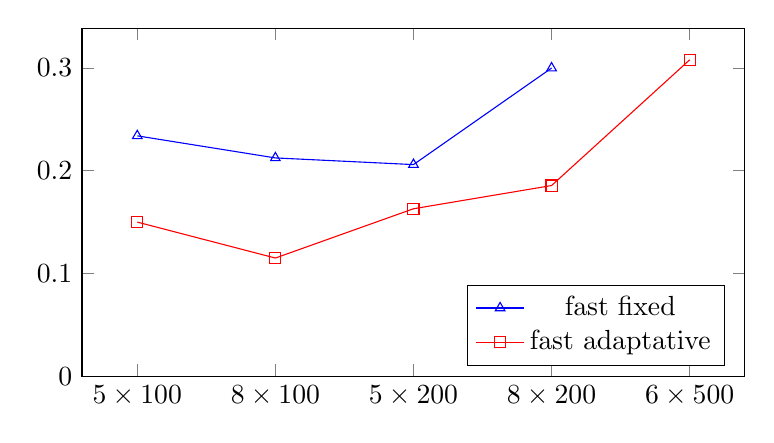
\begin{tikzpicture}
		\begin{axis}[width=10cm,height=6cm,
			xlabel={},
			ylabel={},
			legend pos=south east,
			ymin=0,
			xtick={1,2,3,4,5}, 
			xticklabels={$5\times 100$, $8\times 100$, $5\times 200$, $8\times 200$, $6\times 500$},
			]
			
			
			\addplot[mark=triangle, blue] coordinates {
				(1, 0.234)
				(2, 0.2125)
				(3, 0.206)
				(4, 0.3)
			};
			\addlegendentry{fast fixed}
			
			
			\addplot[mark=square, red] coordinates {
				(1, 0.15)
				(2, 0.115)
				(3, 0.163)
				(4, 0.1856)
				(5, 0.308)
			};
			\addlegendentry{fast adaptative}
			
			
		\end{axis}
	\end{tikzpicture}
	\caption{runtime (seconds per node)}
	\label{fig2}
\end{figure}



We now focus on understanding the potential of {\toolname} for even larger networks than those that are usually considered in the verification community. To this end, Figure~\ref{fig2} presents the  average runtime per node across various DNNS. Observe that while  the average runtime per node isn't fixed (attributable to $\LP(N,K)$), it remains regulated, avoiding exponential increases — from 0.1s per node for the smallest DNN to 0.3s per node for the largest. This suggests that {\toolname} is scalable to larger DNNs, bypassing the high complexity barrier often encountered with approaches such as those based on pure branch and bound.

\fi


\section{Discussion}
\label{Discussion}


In this work, we focused on DNNs employing ReLU activation functions since our approached on usage of MILP, which is naturally suited for ReLU activation function. However, it is worth remarking that the notion of compensation strength is independent of  activation function, and therefore, an interesting direction of future work would be to explore other the impact of compensation strength-based approaches for other activation functions. 


Regarding accuracy, {\toolname} ranks highly among verifiers that abstract values. However, its runtime, particularly for larger DNNs, can be relatively slow, though not excessively so. Numerous optimization avenues exist. A primary strategy involves utilizing $\alpha$-$\beta$-CROWN initially in the sequence, reserving {\toolname} for images unresolved by $\alpha$-$\beta$-CROWN, potentially enhancing this with parallel node computation across additional CPU cores. Another tactic could involve adapting the refined branch-and-bound approach of $\beta$-CROWN to permit {\toolname} to process additional layers beyond MILP's capability, concluding the verification with BaB. More complex strategies might include modifying BaB to branch on unstable ReLU nodes, driven by compensation strength, or analyzing crucial nodes linked to uncertain outputs, enabling quicker computation of less precise bounds for less critical nodes. Furthermore, implementing a Refinement Abstraction framework, akin to methodologies in \cite{atva}, \cite{elboher}, or \cite{SRGR}, could be beneficial.


In terms of neuron correlation, a key feature explicitly encoded by PRIMA, our findings suggest that leveraging compensation strength for network abstraction is generally more effective. Although precise local accuracy is achieved by directly considering ReLU nodes, the accuracy diminishes when correlations originate from distant layers. Retaining a select few significant correlations, in the style of PRIMA, as explicit linear constraints in the MILP model, might offer a strategy to further improve accuracy. 






\section{Conclusion}

In this paper, we introduced the notion of {\em compensating pairs of paths}, with rationale why such a phenomenon creates inaccuracies hard to handle when verifying DNNs. We proved that this phenomenon is actually explaining entirely the inaccuracies, as in their absence, even the simplest Box abstraction (interval arithmetic) suffices to verify accurately DNNs. This is experimentally confirmed by the fact that DNNs harder to verify (verification-agnostic) also exhibit paths with larger compensating strength than  robustly-trained DNNs.

Based on this idea of compensating pairs of paths, we proposed the $\MILP_{Z}$ abstraction considering a subset $Z$ of the set of unstable ReLU nodes, that we proved to be fully accurate if {\em all} the compensating paths are covered by $Z$. Our empirical studies revealed that CMP, selecting $Z$ to cover only {\em a few} paths with the most significant compensation, can yield highly accurate results, up to 20\% more accurate than SOTA within the same runtime, again validating the focus on compensating strength. 
This underscores the potential of compensating strength as an innovative and promising avenue for enhancing DNN verification. We finally proposed several ways to use the compensating strength to optimize current tools in different directions, and leave that as future work.
\newpage

\bibliography{references}
\bibliographystyle{iclr2025_conference}

\newpage

\appendix

\section*{Appendix}

Settings for Hybrid MILP (for Fully Connected DNN, and for CNNs): TO for $\alpha,\beta$-Crown
and number of opens nodes in different layers.



We list some tables and figures comparing $\alpha,\beta$-Crown with other method, from literature.

\subsubsection*{PRIMA} 

PRIMA is one of ERAN's major verifier. Its authors have shown its performance in their paper.

Basically, PRIMA is slightly less accuracy and slower than $\alpha,\beta$-Crown for several networks we considered. Here, we directly use the tables from $\alpha,\beta$-Crown's paper:

\begin{figure*}[h]
	\centering
	\caption{Tables from \cite{crown} to compare $\alpha,\beta$-Crown with earlier verifiers}
	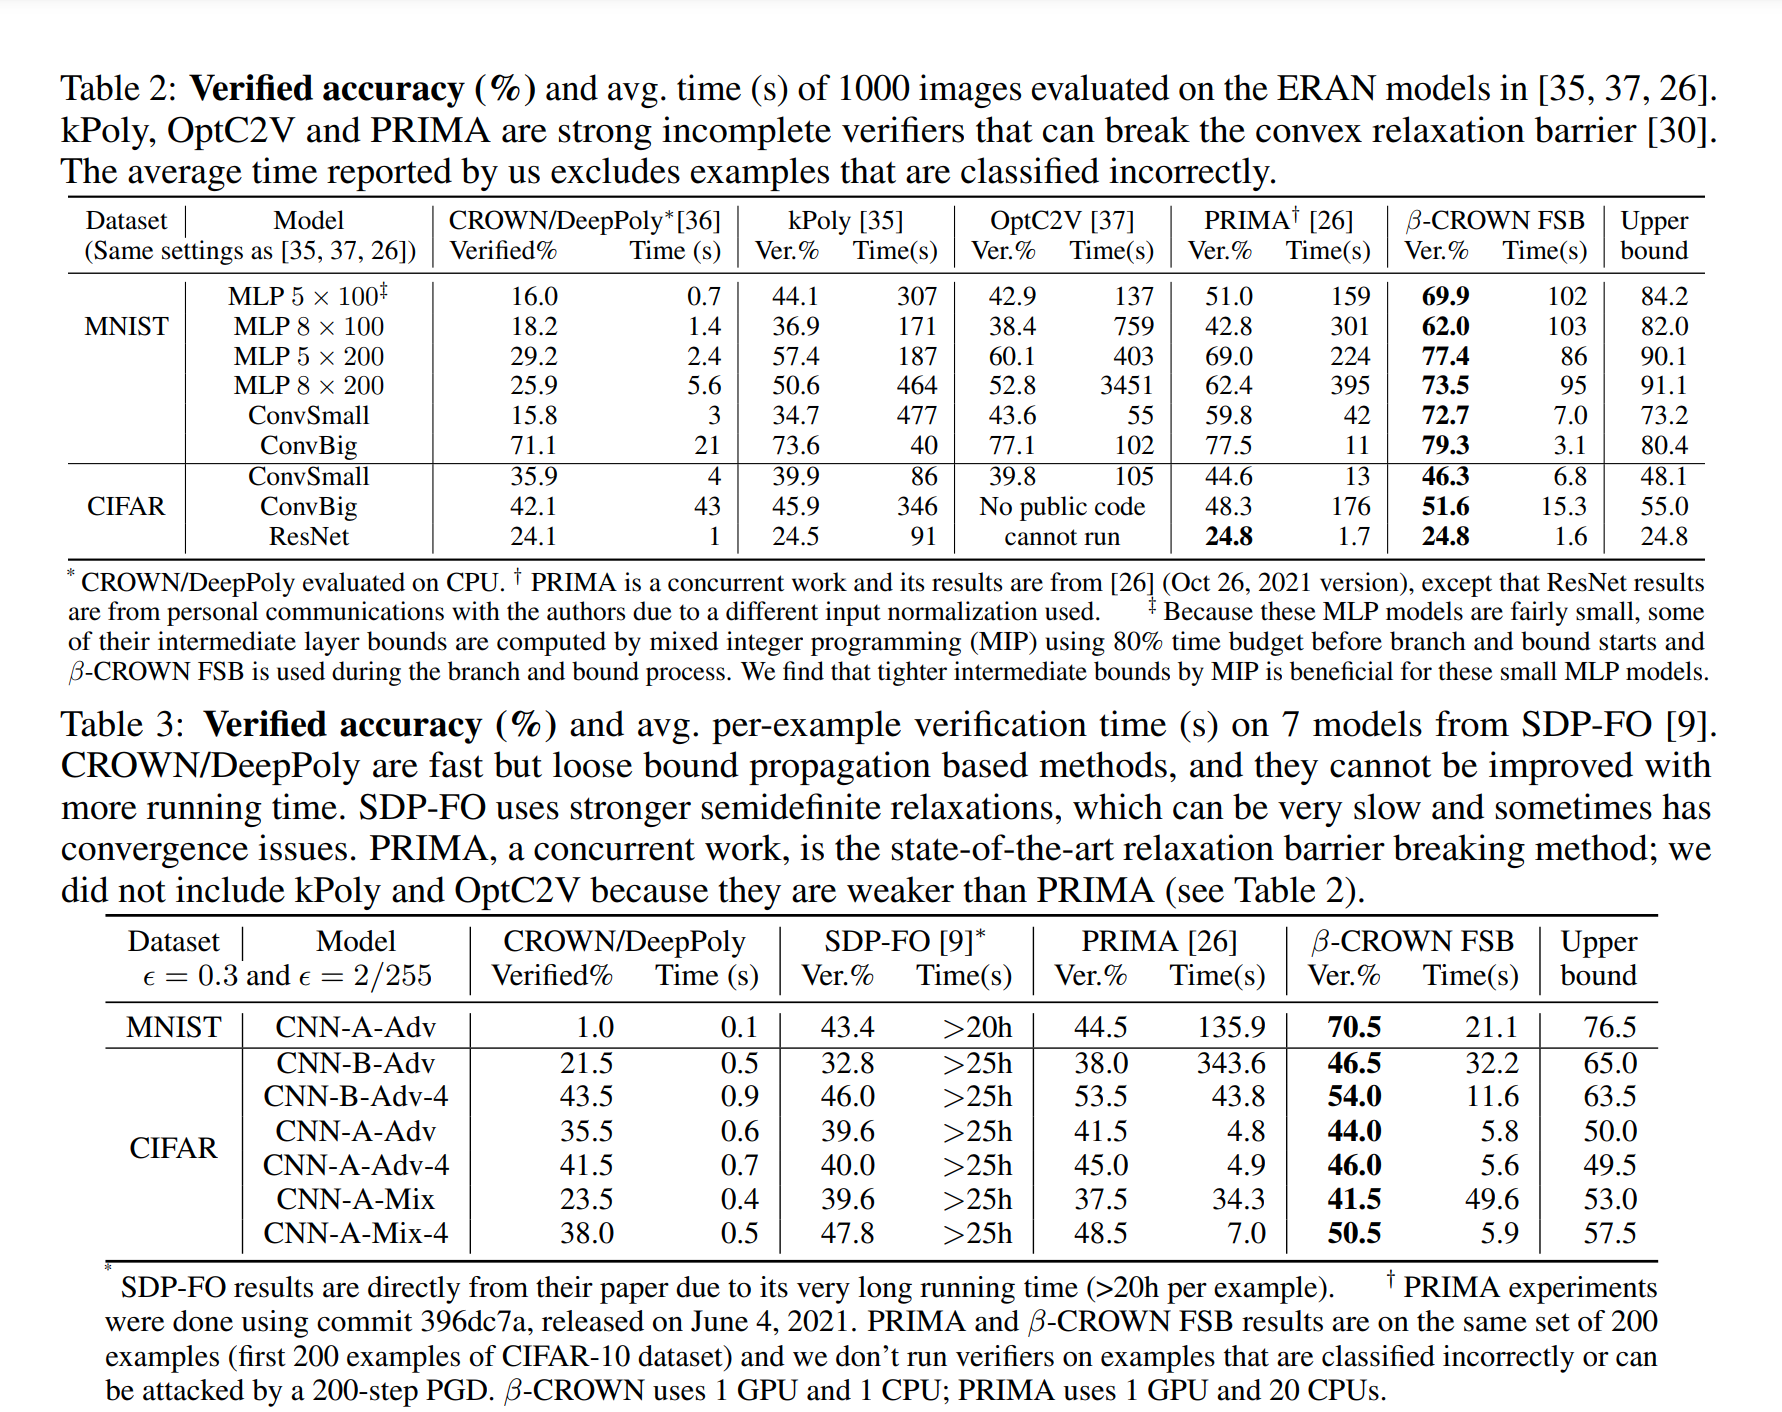
\includegraphics[scale=0.32]{Cronw_PRIMA.png}
\end{figure*}


\subsubsection*{MN-BaB} 


Basically, MN-BaB's performance is close to $\alpha,\beta$-Crown with several kinds of networks. 
\begin{figure}[h]
	\centering
	\caption{A Table from \cite{ferrari2022complete} to compare MN-BaB with $\alpha,\beta$-Crown and other verifiers}
	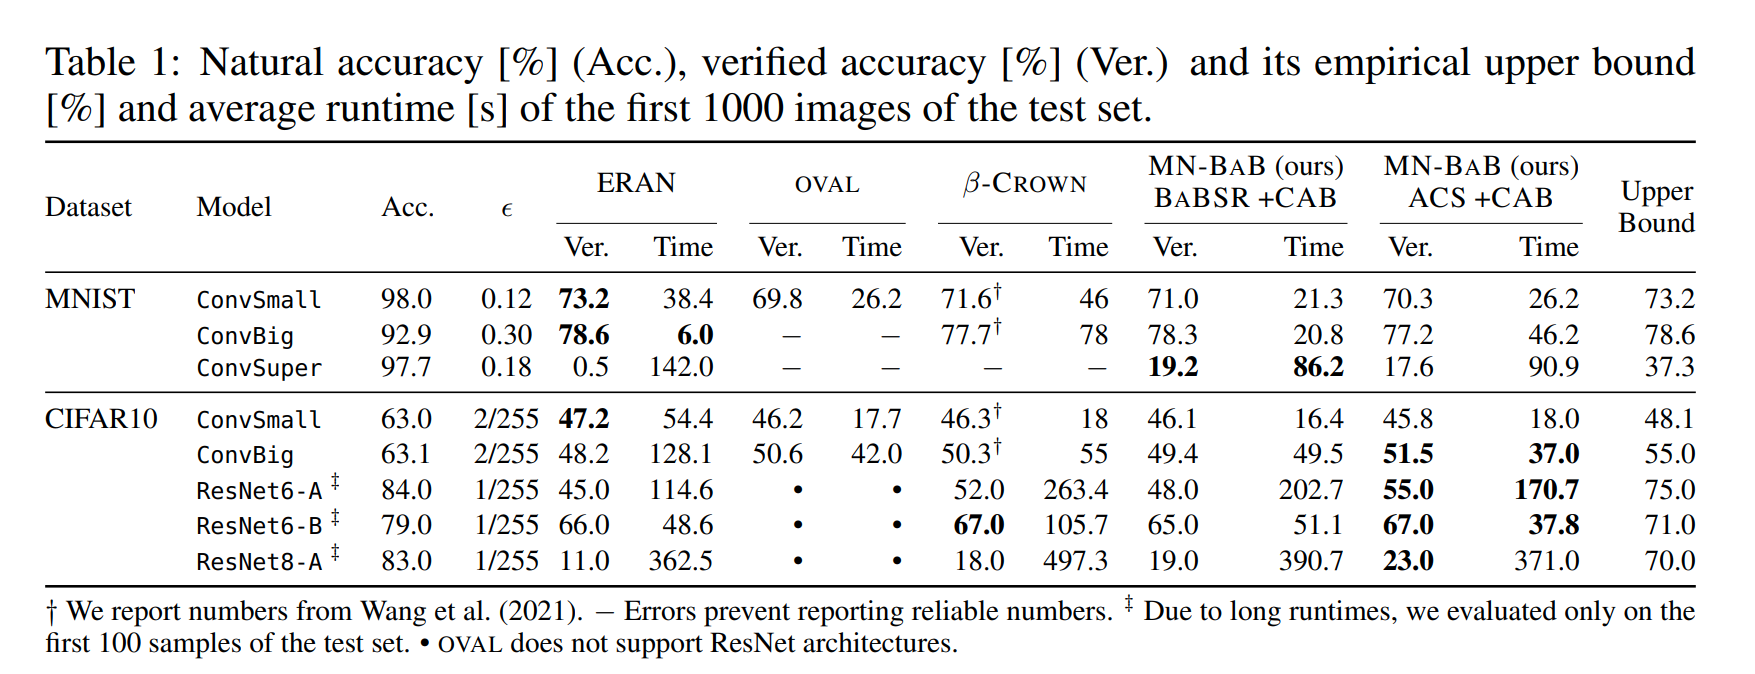
\includegraphics[scale=0.32]{ToMNBAB.png}
\end{figure}

However, the experiments section in their paper does not include those network we focus on. So we run MN-BaB on several networks on our device. The comparison is as follows:

\begin{table}[h]
	\centering
	\begin{tabular}{||l|c|c||c|c||}
		\hline
		Network &  Accuracy & Upper   & MN-BaB &  $\alpha,\beta$-Crown  \\ \hline
		MNIST 6$\times$500 & 99\% & 90\% & $49\%$ & 40 \%    \\
		$\epsilon = 0.035$ & &  &  4995s & 6100s
		\\  \hline
		CIFAR CNN-B-ADV & 99\% & 90\% & $49\%$ & 40 \%    \\
		$\epsilon = 2/255$ & &  &  4995s & 6100s
		\\  \hline
	\end{tabular}
	\caption{}
\end{table}







\subsubsection*{NNenum} 

Similarly, the experiments section in NNenum's paper does not include those network we focus on. So we run NNenum on several networks on our device. 

%As a first step to prove Theorems \ref{th1} and \ref{th2}, 
%we will relax the compensating pairs notion to allows pairs of paths having nodes in common.
%Such a pair is called a {\em weak compensating pair}.
%We will then in a second step prove Theorems \ref{th1} and \ref{th2} for the full definition of compensating pairs of paths.
%
%Let $\cal B$ be a neighbourhood of an input.
%For convenience,
%when the neighbourhood $\cal B$ is clear, 
%we will write $\max(n)$ to denote $\max_{\vx \in \cal B}(\Val_{\vx}(n))$, and $\min(n)$ to denote $\min_{\vx \in \cal B}(\Val_{\vx}(n))$.
%Notice that if $\Val_{\vx}(b)$ is maximal (resp. minimal), 
%then $\Val_{\boldsymbol{x}}(\hat{b})$ also gets maximal (resp. minimal), for $\hat{b}=\texttt{ReLU}(b)$. 
%
%
%We fix a target node $z$.
%We now define the partial influence sign function $S^z$, denoted $S$ when $z$ is clear from the context:
%
%\begin{definition}
%	\label{sign_of_nodes}
%	We define the partial influence sign function $S$ on node $n$: 	
%	\begin{enumerate}
%		\item $S(n)=0$ if all path from $n$ to $z$ have weight $0$; 
%		\item $S(n)=1$ if all path from $n$ to $z$ have non-negative weight, and at least one path has a positive weight; 
%		\item $S(n)=-1$ if all path from $n$ to $z$ have non-positive weight, and at least one path has a negative weight. 
%	\end{enumerate}
%\end{definition}
%
%In general, $S$ may not be defined on every node 
%(e.g. if there is a negative and a positive path from $a$ to $c$). 
%However, if there is no compensating pair of paths, 
%$S$ is defined on all nodes: any node fulfills one of the above cases (1),(2),(3).
%
%For instance for any 3 layer DNN: for an input node $a_i$:
%\begin{enumerate}
%	\item  $S(a_i)=0$ if 
%	for all $b_j, W_{a_i b_j}\cdot W_{b_j c} = 0$
%	
%	
%	\item  $S(a_i)=1$ if for all $b_j, W_{a_i b_j}\cdot W_{b_j c} \geq 0$ and there exists 
%	$j, W_{a_i b_j}\cdot W_{b_j c} > 0$
%	
%	\item $S(a_i)=-1$ if for all $b_j\ W_{a_i b_j}\cdot W_{b_j c} \leq 0$ and there exists 
%	$j, W_{a_i b_j}\cdot W_{b_j c} < 0$ 
%\end{enumerate}
%
%For $b_j$ in the hidden layer, we have $S(b_j)=1,-1,0$ if $W_{b_j c}$ is positive, negative, or 0 respectively. Finally, for the output node $z$, we define $S(z)=1$.
%
%
%
%
%
%\section{Proof of Theorem \ref{th1}}	
%
%
%Assume that there is no (weakly) compensating pair of paths.
%
%
%\begin{lemma}
%	\label{lemma1}
%	Let $L,L'$ be consecutive layers of a DNN without compensation, 
%	$m\in L$ and $n\in L'$. If $W_{m n} \neq 0$ and $S(n) \neq 0$, then 
%	$S(m)=S(n)\mathrm{Sign}(W_{n m})$.
%\end{lemma}
%
%\begin{proof}
%	If $S(n) \neq 0$, then there is a path $\pi$ from $n$ to the output node $z$ with a nonzero weight of the same influence sign as $S(n)$. 
%	So there is a non zero path from $m$ to $z$: $(m n) \pi$, whose influence sign is 
%	$S(n)\mathrm{Sign}(W_{n m})$. As there is no compensation, $S(m)=S(n)\mathrm{Sign}(W_{n m})$.
%	\hfill $\square$
%\end{proof}
%
%
%%For a node $n$, we use $n_s$ to denote $S(n)\cdot n$. 
%%Notice that for $S(n)=1$, $n_s$ gets maximal value whenever $n$ gets maximal value; 
%%while for $S(n)=-1$, $n_s$ gets maximal value whenever $n$ gets minimal value (and vice versa). For $S(n)=0$, $n_s=0$ and thus always reach his minimal and maximal.
%
%Using the concept of influence sign, we introduce input vectors $\vx^{*}, \vx^{\sharp}$: 
%
%\begin{definition}
%We define the following two input vectors $\vx^{*}, \vx^{\sharp}$ in $\cal B$: 
%	\begin{itemize}
%		\item $\vx^{*}$ is the input vector defined in the following way:
%		\begin {itemize}
%		 \item $x^*_{a_i}=\max(a_i)$ if $S(a_i)\in \{0,1\}$, and
%          \item $x^*_{a_i}=\min(a_i)$ otherwise, that is when $S(a_i)=-1$.
%	\end{itemize}
%		
%		\item $\vx^{\sharp}$ is the input vector defined in the following way:
%		\begin{itemize}
%			\item $x^{\sharp}_{a_i}=\min(a_i)$ if $S(a_i)\in \{0,1\}$, and
%			\item $x^{\sharp}_{a_i}=\max(a_i)$ otherwise, that is when $S(a_i)=-1$.
%		\end{itemize}
%	\end{itemize}
%\end{definition}
%
%{Notice that above definitions only involve weights, and do not use bias. As demonstrated by the following lemmas and proofs, our discussion is independent of bias, regardless of whether the bias values are very large or very small.}
%
%We can then prove the following key lemma for Theorem \ref{th1}.
%
%\begin{lemma}
%	\label{lem:key1}
%	\label{lemma2}
%For all $n$ with $S(n)=1$, we have $\val_{\vx^*}(n) = \max(n)$
%and $\val_{\vx^{\sharp}}(n) = \min(n)$.
%For all $n$ with $S(n)=-1$, we have $\val_{\vx^*}(n) = \min(n)$
%and $\val_{\vx^{\sharp}}(n) = \max(n)$. Further, for $L,L'$ two consecutive layers and $n$ on layer $L'$:
%$$\max(n)=\sum_{m \in L, W_{mn}>0}W_{mn} \max(\hat{m}) + \sum_{m \in L, W_{mn}<0}W_{mn} \min(\hat{m}) + bias_n$$
%$$\min(n)=\sum_{m \in L, W_{mn}>0}W_{mn} \min(\hat{m}) + \sum_{m \in L, W_{mn}<0}W_{mn} \max(\hat{m}) + bias_n$$
%
%\end{lemma}
%
%\begin{proof}
%	We prove this lemma by induction on layers. For input layer, this is true by definition. Suppose this lemma is true up to layer $L_i$, we need to show this for layer $L_{i+1}$. Let $n$ be a node in layer $L_{i+1}$, then by definition, we have the following equation: \begin{align*}
%		\val_{\vx}(n) = \sum_{m\in L}W_{m n}\val_{\vx}(\hat{m})) + bias_n.
%	\end{align*}
%	
%	By induction hypothesis, when input vector is $\vx^{*}$, for every $m$, if $S(m)=1$, then $\Val_{\vx^*}(\hat{m})=\max(\hat{m})$ and if $S(\hat{m})=-1$, then $\Val_{\vx^*}(\hat{m})=\min(\hat{m})$. Assume that $S(n)=1$. By applying Lemma \ref{lemma1} and the induction hypothesis:
%	\begin{align*}
%		\val_{\vx^*}(n) = \sum_{m \in L_i, W_{mn}>0}W_{mn} \max(\hat{m}) + \sum_{m \in L_i, W_{mn}<0}W_{mn} \min(\hat{m}) + bias_n\\
%	\end{align*}
%	
%
%
%	Further, we have the following inequality:
%	\begin{align*}
%		\max(n)\leq & \sum_{m \in L_i, W_{mn }>0}W_{mn} \max(\hat{m}) + \sum_{m \in L_i, W_{mn}<0}W_{mn} \min(\hat{m}) + bias_n\\
%		\leq & \val_{\vx^*}(n)
%	\end{align*}
%	
%	%If $S(m)=1$, then by Lemma \ref{lemma1}, $W_{mn}>0$; if $S(m)=-1$, then $W_{mn}<0$; if $S(m)=0$, then $W_{mn}=0$.
%	
%	By definition of $\max$, we have $\val_{\vx^*}(n) \leq \max(n)$.
%	Combining the 2 formulas, we obtain $\max(n)=\Val_{\vx^*}(n)$. 
%	
%	We prove similarly that $\min(n)=\Val_{\vx^\sharp}(n)$,
%	and the case $S(n)=-1$. This concludes the induction. 
%\end{proof}
%
%{ As we mentioned earlier, this proof does not have any requirements on the bias.}
%
%\iffalse
%	As direct corollary of Lemma \ref{lem:key1}, we obtain:
%	
%	\begin{corollary}
%		\label{cor1}
%		$$\max(c)=\sum_{b \in L, W_{bc}>0}W_{bc} \max(\hat{b}) + \sum_{b \in L, W_{bc}<0}W_{bc} \min(\hat{b}) + bias_c$$
%		$$\min(c)=\sum_{b \in L, W_{bc}>0}W_{bc} \min(\hat{b}) + \sum_{b \in L, W_{bc}<0}W_{bc} \max(\hat{b}) + bias_c$$
%	\end{corollary}
%	
%\fi
%	
%	%Notice that for all $x$, for either $S(c)=1$ or $S(c)=-1$, these two bounds are found in Lemma \ref{lemma2},
%	%from configuration $\boldsymbol{x}^*$ and $\boldsymbol{x}^\sharp$.
%	
%	
%	
%	
%	
%	\subsubsection*{Bounds generated by Value Abstraction}
%
%	\smallskip
%	
%	Let $[\alpha_n,\beta_n]$ be the bounds generated by the Box abstraction.
%	We show that these bounds are exact when there is no (weak) compensating pairs of paths, i.e. for all node $n$ of the DNN, we have $\alpha_n=\min(n)$ and $\beta_n=\max(n)$.
%
%\begin{proof}
%	 We show that inductively. The initialization is obvious as Box Abstraction is always exact for the first layer.
%
%	Let $n$ be node of the DNN. We set the target $z=n$ and consider the influence sign function $S^z=S^n=S$ corresponding to that node. By definition, $S(n)=1$. 
%	
%	The Box abstraction computes its upper bound using:
%	$$\beta_n= \sum_{W_{mn}>0} W_{mn} \beta_{\hat{m}} + \sum_{W_{mn}<0} W_{mn} \alpha_{\hat{m}} + bias_n$$
%
%	By induction hypothesis, we have 
%		$\beta_{\hat{m}}=\max(\hat{m})$ and
%		$\alpha_{\hat{m}}=\min(\hat{m})$, thus 
%		applying the second part of Lemma \ref{lem:key1}, we obtain
%		$\beta_n=\max(n)$.
%		
%		Similarly, we obtain $\alpha_n=\min(n)$.
%		
%		Consider now $\alpha_{\hat{n}},\beta_{\hat{n}}$.
%		If $\alpha \leq 0$ then $\alpha_{\hat{n}}=0=\max(\hat{n})$.
%		Otherwise, $\alpha_{\hat{n}}=\alpha_n=\max(\hat{n})$.
%		In both case it is exact.
%
%		Similarly, if $\beta_n=\max(n)<0$, 
%		then $\beta_{\hat{n}}=\max(\hat{n})=0$, 
%		and otherwise 
%		$\beta_{\hat{n}}=\max(\hat{n})=\beta_n=\max(n)$.
%		
%		Hence we have equality pre and post activation function.
%			\end{proof}
%	
%
%
%This shows the statement of Theorem 1 with the weaker statement that there is no weak compensating pairs of paths.
%
%	
%	
%	\subsubsection*{From weak to normal}
%	
%	\begin{lemma}
%		If a DNN has no compensating pair, then it also does not have weak compensating pair from an input node to the output node.
%	\end{lemma}
%	
%	\begin{proof}
%		By contradiction, if there is a weak compensating pair of two paths, $\rho_1,\rho_2$, 
%		then consider the common nodes by increasing layer $n_1 \cdots n_k$ in $\rho_1,\rho_2$ (including the initial and final nodes).
%		Assume that there is no compensating pair.
%		It means that all the segment of $\rho_1,\rho_2$ from $n_i$ to $n_{i+1}$ have the same influence sign (they have no nodes in common but the initial and final nodes).
%		Hence $\rho_1$ and $\rho_2$ have the same influence sign, a contradiction with $\rho_1,\rho_2$ being a weakly compensating pair. 
%	\end{proof}
%	
%	This finishes the proof of Theorem \ref{th1}.
%	
%	
%
%
%
%
%
%
%\newpage
%
%
%
%
%
%	
%
%
%
%
%
%			
%\section{Proof of Theorem \ref{th2}}
%			
%			In this section, we will prove theorem \ref{th2}. We first prove the following weaker theorem:
%			
%			\begin{theorem} \label{thm:2}	
%				Suppose $\mathcal{D}$ is a DNN with a unique output node $z$.
%				Let $X$ be the set of nodes $n$ such that there is a weak compensating path 
%				passing by $n$ (except its source and target nodes).
%				Then $\MILP_X$ computes the exact bounds $[\alpha,\beta]$ for $z$,
%				i.e. $\alpha=\min(z)$ and $\beta=\max(z)$.
%			\end{theorem}
%			
%			
%			\subsection{Proof of Theorem \ref{thm:2}}
%			
%			\begin{definition}
%				We define a partition of the set $A$ of input nodes as $A_{zero} \sqcup A_{pure}\sqcup A_{open}$, with:  
%				\begin{itemize}
%					\item $A_{zero}= \{a \mid \forall \text{ path $\rho$ from $a$ to } z, weight(\pi)=0\}$.
%	
%					\item $a_k \in A_{pure}$  if $a \notin A_{zero}$ and either
%					\begin{enumerate}
%						\item every path from $a_k$ to $z$ has weight $\geq 0$, or
%						\item every path from $a_k$ to $z$ has weight $\leq 0$. 
%						
%					\end{enumerate}
%					Hence, $a_k$ is not a source of a weak compensating pair. We denote 
%					$A_{pure}$ by $I$ for short.
%					\item $a_k \in A_{open}$ iff $a_k \notin A_{pure} \sqcup A_{zero}$, that is there exists two paths $\rho,\rho'$ from $a_k$, one with positive and one with negative weight. 	We denote $A_{open}$ by $J$ for short.
%				\end{itemize}
%			\end{definition} 
%			
%
%			
%			\begin{lemma} \label{lem:open_node_2}
%				A node $b$ in a hidden layer will not be on a weak compensating path if and only if one of the following happens:
%				\begin{enumerate}
%					\item Any path from $b$ to the output node $z$ has a weight $0$, and we use $weight({bz})=0$ to denote this case, or
%					\item For every input node $a_j\in J$, every path from $a_j$ to $b$ has a weight of $0$. We use $weight({a_jb})=0$ to denote this case.
%				\end{enumerate}
%				
%			\end{lemma}
%			
%			We denote $B_{zero}$ the set of nodes $b$ that case 1 holds, and denote $B_{pure}$ the set of nodes $b$ such that case 2 holds but case 1 does not hold.
%			We denote $B_{open}$ the set of all nodes $b$ in a weak compensating path (remaining cases).
%			
%		{ 	Similarly, above definitions $A_{zero},A_{open}, A_{pure}$ and $B_{zero},B_{open},B_{pure}$ do not consider bias, and any kind of bias will not affect our theorem.}
%		
%		\begin{figure}[h]
%			\centering
%			\begin{tikzpicture}[>=stealth, node distance=2cm]
%				% Input nodes (two types)
%				\node[circle, draw, minimum size=0.5cm] (input1) at (-1,0) {$a_0$};
%				\node[circle, draw, minimum size=0.5cm] (input2) at (-2,0) {$a_1$};
%				\node[circle, draw, minimum size=0.5cm] (input3) at (-4,0) {$a_2$};
%				
%				\node[circle, draw, minimum size=0.5cm] (input4) at (-5,0) {$a_3$};
%				\node[circle, draw, minimum size=0.5cm] (input5) at (-7,0) {$a_4$};
%				\node[circle, draw, minimum size=0.5cm] (input6) at (-8,0) {$a_5$};
%				
%				\draw[draw=black, dashed] (-1.5,0) ellipse (1.35 and 0.75);
%				\node[below] at (-1.5,-0.75) {$A_{zero}$};
%				
%				\draw[draw=black, dashed] (-2,2) ellipse (0.75 and 0.75);
%				\node[right] at (-1,2) {$B_{zero}$};
%				
%				% Hidden layer nodes
%				
%				\node[circle, draw, minimum size=0.5cm, fill=blue!20] (hidden1) at (-2,2) {$n_0$};
%				
%				\node[circle, draw, minimum size=0.5cm, fill=blue!20] (hidden2) at (-4,2) {$n_1$};
%				\node[circle, draw, minimum size=0.5cm, fill=blue!20] (hidden3) at (-5,2) {$n_2$};
%				
%				\node[circle, draw, minimum size=0.5cm, fill=blue!20] (hidden4) at (-7,2) {$n_3$};
%				\node[circle, draw, minimum size=0.5cm, fill=blue!20] (hidden5) at (-8,2) {$n_4$};
%				
%				
%				
%				\draw[draw=black, dashed] (-4.5,0) ellipse (1.35 and 0.75);
%				\node[below] at (-4.5,-0.75) {$A_{pure}$};
%				
%				
%				\draw[draw=black, dashed] (-7.5,0) ellipse (1.35 and 0.75);
%				\node[below] at (-7.5,-0.75) {$A_{open}$};
%				
%				
%				
%				\draw[draw=black, dashed] (-4.5,2) ellipse (1.35 and 0.75);
%				\node[left] at (-3.5,3) {$B_{pure}$};
%				
%				
%				\draw[draw=black, dashed] (-7.5,2) ellipse (1.35 and 0.75);
%				\node[left] at (-8.5,1.5) {$B_{open}$};
%				
%				
%				
%				% Output node
%				\node[circle, draw, minimum size=0.8cm, fill=red!20] (output) at (-5,4) {$z$};
%				
%				
%				% connections
%				
%				\draw[->] (input1) -- (hidden1);
%				
%				\draw[->] (input3) -- (hidden5);
%				
%				\draw[->] (input4) -- (hidden4);
%				
%				
%				%		% Connect input to hidden layer
%				\foreach \i in {3,4} {
%					\foreach \h in {3,2} {
%						\draw[line width=1.5pt, ->] (input\i) -- (hidden\h);
%					}
%				}
%				
%				
%				\foreach \i in {5,6} {
%					\foreach \h in {4,5} {
%						\draw[->] (input\i) -- (hidden\h);
%					}
%				}
%				%		
%				% Connect hidden layer to output
%				\foreach \h in {2,3} {
%					\draw[line width=1pt,->] (hidden\h) -- (output);
%				}
%				
%				\foreach \h in {4,5} {
%					\draw[->] (hidden\h) -- (output);
%				}
%				
%				%\		% Input label
%				\node[left=0.7cm of input6] {Input Layer};
%				
%				% Hidden label
%				\node[left=0.7cm of hidden5] {Hidden Layer};
%				
%				% Output label
%				\node[left=0.5cm of output] {Output Layer};
%			\end{tikzpicture}
%			\caption{Definitions in the proof of Theorem \ref{th2}}
%			\label{fig:neural_network_types_simplified}
%		\end{figure}
%			
%			\begin{proof}
%				First, we show that if one of case 1, 2 happens, then $b$ will not be in a weak compensating pair. If 1), it is obvious. For 2, we reason by contradiction: assume there is a pair of weak compensating paths 	$(\pi,\pi')$ starting with $a$, with $b$ in $\pi$ and weight$(\pi) > 0$. It means that $a \in J$. This is a contradiction as 2) $weight({a_j,b})=0$ implies weight$(\pi)=0$.
%				
%				Second, we show that if neither 1 nor 2 hold, then $b$ will be in a weak compensating path.
%				Because 2) does not hold, there exists $a_j \in J$ with $weight({a_j,b}) \neq 0$, say $>0$.
%				Because 1) does not hold, $weight({b,z}) \neq 0$, say $>0$.
%				Now, by definition of $J$, there is a pair of weak compensating paths $\pi,\pi'$ 
%				from $a_j$ to $z$, say with $\pi'$ with weight $<0$.
%				Then two paths $(a_j,b,z)$ and $\pi'$ also form a weak compensating pair.
%			\end{proof}
%			
%						
%			
%			\begin{lemma}\label{lem:subnetwork}
%				$I \cup B_{pure} $ forms a sub-network, denoted $D_I$. That is, 
%				for $n \in B_{pure}$, for every path $\rho$ from $m$ to $n$
%				either $m \in B_{pure}\cup I$ or $weight(\rho)=0$.
%				Further, in $D_I$, there is no (weakly) compensating pair.
%			\end{lemma}
%
%			
%
%			
%			\begin{proof}
%				This is simply because for a node $c\in B_{pure}$ in a hidden layer or the output layer, for a node $b$ in one layer before, if $b\notin B_{pure}\cup I$, then:
%				
%				1. if $b\in J$, by definition, $W_{bc}=0$.
%				
%				2. if $b\in B_{open}$, then $W_{bc}=0$; otherwise there exists $<a_j,b,c>$ a path from $a_j\in J$ to $c$ with a nonzero value, a contradiction.
%				
%				3. if $b\in B_{zero}$, then $W_{bc}=0$; otherwise there exists $<b,c,z>$ a path from $b$ to $z$ the output node with a nonzero value, a contradiction. 
%			\end{proof}
%			
%			
%			
%			For an input $\vx$ and a subset $S$ of input nodes, we denote by 
%			$\boldsymbol{x}_S$ to refer the input vector $\langle x_{a_k}\rangle_{a_k\in S}$. We use $\boldsymbol{x}_I\oplus \boldsymbol{x}_J = \boldsymbol{x}$ and 
%			$\Val_{\boldsymbol{x}_I,\boldsymbol{x}_J} (z)=\Val_{\boldsymbol{x}}(z)$. 
%			
%			
%			Invoking Lemma \ref{lem:subnetwork}, we can apply Theorem 1 on $D_I$, and obtain two input vectors $\boldsymbol{x}_I^*,\boldsymbol{x}_I^{\sharp}$ on $I$
%			minimizing and maximizing all the nodes in $D_I$.
%
%			\smallskip
%
%		
%			Recall the influence sign function of nodes from Definition \ref{sign_of_nodes}. 
%			Because weakly compensating paths are allowed, the influence sign function is no longer defined on all nodes. $S$ is defined for all nodes from which there is no weakly compensating pairs of paths to $z$. In particular, $S$ is defined on all nodes of $I$.
%
%			\begin{lemma}\label{lem:sign}
%				Let $m,n$ be two nodes, such that $S$ is defined on $m$ and there is a path $\rho$ with non zero weight to a node $n$. Then $S$ is defined on $n$
%				 (there is no compensating pair of paths from $n$ to $z$).
%				Further, $S(n)= Sign(weight(\rho)) S(m)$.
%			\end{lemma}
%			
%			\begin{proof}
%				By contradiction, assume that there exists two paths $\rho_1,\rho_2$ from 
%				$n$ to $z$ with (strictly) different influence signs. The pair $\langle a_i,n\rangle \cdot \rho_1$ and $\langle a_i,n\rangle \cdot \rho_2$ is compensating, a contradiction with $a_i\in I$. 
%			\end{proof}
%
%			Hence, for all node $n$, either $S$ is defined on $n$, or 
%			$n$ depends only upon input nodes in $J$.
%			Let us call $D_J$ the set of such nodes which only depends upon nodes in $J$.
%			$D_J$ forms a sub-network.
%			$D_J$ contains the set of all nodes from which there is a weakly compensating pair of paths to $z$.
%			By definition, for any $b\in D_J$, either $b\in B_{open}$, or $b$ is a constant node: any path from any input node must have zero weight to it.
%			For a node $b$ for which $S$ is undefined, $b$ thus only depends on $J$; so, if $\boldsymbol{x}_J$ is fixed, then the value of $b$ will be fixed.
%			Notice that $D_I \sqcup D_J$ does not cover the DNN entirely in general.
%			
%			
%			
%			\begin{lemma} \label{lem:reach_max_2}
%				Let $n$ be a node on which $S$ is defined. If $S(n)=1$,
%				for any valuation $\boldsymbol{x}^0_J$,	we have: 
%				$$\max_{\boldsymbol{x}_I} (\Val_{\boldsymbol{x}_I,\boldsymbol{x}^0_J}(b)) =  \Val_{\boldsymbol{x}_I^*,\boldsymbol{x}^0_J}(b).$$
%				
%				$$\min_{\boldsymbol{x}_I} (\Val_{\boldsymbol{x}_I,\boldsymbol{x}^0_J}(b)) =  \Val_{\boldsymbol{x}_I^{\sharp},\boldsymbol{x}^0_J}(b).$$
%				
%				
%				If $S(b)=-1$, 
%				$$\max_{\boldsymbol{x}_I} (\Val_{\boldsymbol{x}_I,\boldsymbol{x}^0_J}(b)) =  \Val_{\boldsymbol{x}_I^{\sharp},\boldsymbol{x}^0_J}(b).$$
%				
%				$$\min_{\boldsymbol{x}_I} (\Val_{\boldsymbol{x}_I,\boldsymbol{x}^0_J}(b)) =  \Val_{\boldsymbol{x}_I^{*},\boldsymbol{x}^0_J}(b).$$	
%			\end{lemma}
%			
%			\begin{proof}	
%				Fix an input vector $\boldsymbol{x}^0_J$.
%				This also fixes the values in $D_J$.
%				Consider the DNN $D'$ with input nodes $a_i\in I$, where all the 
%				edges from $m \in D_J$ to $n$ are replaced by a bias (equals to the weight of the edge times the fix value $\val_{\boldsymbol{x}^0_J}(m)$) for $n$ (we sum all these bias for a neuron $n$).
%				We denote $\val'$ values of nodes in this DNN $D'$.
%				 
%				We have $\Val_{\boldsymbol{x}_I,\boldsymbol{x}^0_J}(z) = \val'_{\boldsymbol{x}_I}(z)$.
%				In the simplified $D'$, there is no weakly compensating path to $z$ because 
%				$D_J$ contains all the source of weakly compensating path to $z$.
%				Therefore we can apply Lemma \ref{lem:key1} to get that 
%				$\val'_{x_I}(z)$ reaches its maximal value for $\boldsymbol{x}_I=\boldsymbol{x}_I^*$, and conclude by using $\Val_{\boldsymbol{x}_I,\boldsymbol{x}^0_J}(z) = \val'_{\boldsymbol{x}_I}(z)$. The case for min is similar. 
%			\end{proof}
%			
%			From Lemma \ref{lem:reach_max_2}, we immediatly obtain the following corollary:
%
%			\begin{corollary}
%				\label{corr:main}
%			For a node $b$ with $S(b)=1$:
%		
%			$$\max(b)=\max_{\vx_J} \val_{\vx^{\star}_I,\vx_J}(b)$$
%			$$\min(b)=\min_{\vx_J} \val_{\vx^{\sharp}_I,\vx_J}(b)$$
%			and for $S(b)=-1$:
%	
%			$$\max(b)=\max_{\vx_J} \val_{\vx^{\sharp}_I,\vx_J}(b)$$
%			$$\min(b)=\min_{\vx_J} \val_{\vx^{\star}_I,\vx_J}(b)$$
%			\end{corollary}
%			
%	
%			
%
%
%			%\subsection{$\MILP_X$ is accurate}
%			
%			
%
%
%
%
%
%			%We want to show that $\beta= \max(z)$. 
%			%As the MILP abstraction is a sound over-approximation, it suffices to show that %$\beta\leq \max (z)$.
%			%The case for $\alpha$ is similar.
%			
%			
%			%\begin{lemma}
%			%	Both $D_I$ and $D_J$ are accurate in the sense that for any $b$ in $D_I$ or %$D_J$, $\UB(b)=\max(b)$ and $\LB(b)=\min(b)$.
%			%\end{lemma}
%			
%			%\begin{proof}
%			%	For $D_I$, it is because of no compensating as proved in the first section. %For $D_J$, it is because all nodes are either opened or constants. 
%			%\end{proof}
%			
%			
%			%\begin{definition} Assume $\boldsymbol{x}^0_I\oplus \boldsymbol{x}^0_J$ is a input vector, and $b$ is node in hidden layers or output layer.
%			%
%			%	1. For a given vector $\boldsymbol{x}$ , $\B_{\boldsymbol{x}^0_I, \boldsymbol{x}^0_J, \boldsymbol{x}}(b)$ is the value of $b$ in the MILP model for values $\boldsymbol{x}^0_I, \boldsymbol{x}^0_J, \boldsymbol{x}$.
%			%\end{definition}
%\iffalse			
%			For input vectors $\boldsymbol{x}^0_I,\boldsymbol{x}^0_J$, let $\UB_{\boldsymbol{x}^0_I,\boldsymbol{x}^0_J}(b)$ be the upper bound in the above fixed formulation and framework while the input $\boldsymbol{x}^0_I,\boldsymbol{x}^0_J$ is fixed: that is, besides the constraints in above MILP models, we add new constraints $\boldsymbol{x}_I,\boldsymbol{x}_J=\boldsymbol{x}^0_I,\boldsymbol{x}^0_J$. We  define $\LB_{\boldsymbol{x}^0_I,\boldsymbol{x}^0_J}(b)$ similarly for $\LB$ lower bound. For them, we have the following lemma:
%			
%			\begin{lemma} In an MILP formulation, for a node $c$ in a hidden layer or output layer:
%				
%				1. $\UB(b)=\max_{\boldsymbol{x}^0_I,\boldsymbol{x}^0_J}\UB_{\boldsymbol{x}^0_I,\boldsymbol{x}^0_J}(c)$. 
%				
%				2. $\LB(b)=\min_{\boldsymbol{x}^0_I,\boldsymbol{x}^0_J}\LB_{\boldsymbol{x}^0_I,\boldsymbol{x}^0_J}(c)$. 
%			\end{lemma}
%			
%			\begin{proof}
%				This is by the definition of MILP formulation and $\UB_{\boldsymbol{x}^0_I,\boldsymbol{x}^0_J}, \LB_{\boldsymbol{x}^0_I,\boldsymbol{x}^0_J}$. 
%			\end{proof}
%			
%	
%			
%			
%		%We will prove this by induction on layers from the first hidden layer to the output layer. More specifically, we will prove the following lemmas:
%			
%	
%
%		\begin{lemma} \label{lem:main}
%				For any node $c$ in a hidden layer or the output layer, if $c\notin B_{zero}$, then:		\begin{enumerate}
%					\item for any fixed $\boldsymbol{x}^0_J$, when  $\boldsymbol{x}_I=\boldsymbol{x}^*_I$, the value for $c$ in the MILP model is a fixed number, and naturally $\UB_{\boldsymbol{x}^*_I,\boldsymbol{x}^0_J}(c)=\LB_{\boldsymbol{x}^*_I,\boldsymbol{x}^0_J}(c)$. The same is true for $\boldsymbol{x}^\sharp_I$.
%					
%					\item for any fixed $\boldsymbol{x}^0_J$, if $S(c)=1$, then $$\max_{\boldsymbol{x}_I} \UB_{\boldsymbol{x}_I,\boldsymbol{x}^0_J}(c)=\UB_{\boldsymbol{x}^*_I,\boldsymbol{x}^0_J}(c)= \Val_{\boldsymbol{x}^*_I,\boldsymbol{x}^0_J}(c) = \max_{\boldsymbol{x}_I} \Val_{\boldsymbol{x}_I,\boldsymbol{x}^0_J}(c).$$ The similar for $S(c)=-1$, $\langle \LB,\min\rangle$, $x^\sharp_I$: we can change two of them at the same time.
%					
%					\item Therefore, $\UB(c)=\max(c)$ and $\LB(c)=\min(c)$.
%				\end{enumerate}
%				
%				
%				
%			\end{lemma}
%			
%
%
%			\begin{proof}
%				We prove this lemma by induction on layers. For first hidden layer $L_1$, it is obvious. Suppose we have proved part 1,2,3 up to layer $L_i$, then for layer $L_{i+1}$, suppose $c$ is a node in this layer. 
%				
%				(1)	If $S(c)$ is undefined, then by previous discussion, $c$ is in a sub-network from $J$ with all nodes opened; and if $\boldsymbol{x}_J=\boldsymbol{x}_J^0$ is fixed, then in the MILP model, the value for $c$ is also fixed. 
%				
%				If $S(c)$ is defined, then consider all $b$ such that $W_{bc}\neq 0$. First, $b$ cannot in $B_{zero}$; so by induction hypothesis, the value of $b$ is fixed under $\boldsymbol{x}^*_I,\boldsymbol{x}^0_J$ in MILP model. 
%				
%				
%				
%				If $b\in B_{open}$, the term is $W_{bc}\ReLU(b)$. We know then by induction hypothesis, the value for $b$ in MILP is a fixed value. Then the term $W_{bc}\ReLU(b)$ is also a fixed number.  
%				
%				If $b\in B_{pure}$, the term is $W_{bc}\mathrm{AppB}(b)$ ($\mathrm{AppB}$ is the LP approximation domain of $\ReLU$) and either $S(b)$ is undefined and $b$ is a constant in the network and so is in the MILP model (trivial case), or $S(b)$ is defined. 
%				
%				Then by induction hypothesis for all 1, 2 and 3 parts,  the value of $b$ in the model is fixed (part 1), and it is equal to $\max_{\boldsymbol{x}_I} \Val_{\boldsymbol{x}_I,\boldsymbol{x}^0_J}(c)$ or $\min_{\boldsymbol{x}_I} \Val_{\boldsymbol{x}_I,\boldsymbol{x}^0_J}(c)$ (by part 2, depending on $S(b)$). Since $b$ only depends on $I$, this value also equal to $\max_{\boldsymbol{x}_I} \Val_{\boldsymbol{x}_I}(c)$ or $\min_{\boldsymbol{x}_I} \Val_{\boldsymbol{x}_I}(c)$, and by induction hypothesis on part 3, equal to $\UB(b)$ or $\LB(b)$. For either of them, $\mathrm{AppB}(b)$ will be fixed value. Hence, in this case, the term $W_{bc}\mathrm{AppB}(b)$ is also a fixed number.
%				
%				Therefore, in the MILP model, $c$ is a sum of terms that are all fixed numbers. Hence $c$ is a fixed number.
%				
%				(2) If $S(c)=1$, then we have the following:	\begin{align*}
%					\mathrm{UB}_{\boldsymbol{x}^0_J,\boldsymbol{x}^0_I}(c) \leq constant + \sum_{b\in B_{open}\cap l_i} W_{bc}\ReLU(\B_{\boldsymbol{x}^0_I,\boldsymbol{x}^0_J}(b)) + \sum_{b\in B_{pure}\cap l_{i}} W_{bc} \mathrm{AppB}(\B_{\boldsymbol{x}^0_I,\boldsymbol{x}^0_J}(b)),
%				\end{align*}where $\B$ means one of $\UB$ or $\LB$ depending on the influence sign of $W_{bc}$: if $W_{bc}$ is positive, then $\UB$, otherwise $\LB$. Notice that all $b$ displayed are that $S(b)$ defined, because if $S(b)$ undefined, then for fixed $\vx_J$, value of $b$ is fixed and will be put into the constant.
%				
%				Now by induction hypothesis part 2, if $S(b)=1$, then $\UB_{\boldsymbol{x}^*_I,\boldsymbol{x}^0_J}(b)=\max_{\vx_I}\UB_{\boldsymbol{x}^*_I,\boldsymbol{x}^0_J}(b)$; and if $S(b)=-1$, $\LB_{\boldsymbol{x}^*_I,\boldsymbol{x}^0_J}(b)=\min_{\vx_I}\LB_{\boldsymbol{x}^*_I,\boldsymbol{x}^0_J}(b)$. Moreover, since $S(c)=1$, $S(b)$ and $W_{bc}$ have the same influence sign. And both $\ReLU$ and $\mathrm{AppB}$ are non-decreasing functions. Combining all these facts, we have:\begin{align*}
%					\mathrm{UB}_{\boldsymbol{x}^0_J,\boldsymbol{x}^0_I}(c)\leq 
%					&constant + \sum_{b\in B_{open}\cap l_i} W_{bc}\ReLU(\B_{\boldsymbol{x}^*_I,\boldsymbol{x}^0_J}(b)) + \sum_{b\in B_{pure}\cap l_{i}} W_{bc} \mathrm{AppB}(\B_{\boldsymbol{x}^*_I}(b))\\
%					= & \mathrm{UB}_{\boldsymbol{x}^0_J,\boldsymbol{x}^*_I}(c). 
%				\end{align*}  This is the first equal.
%				
%				The second is simply because $\UB_{\boldsymbol{x}^*_I,\boldsymbol{x}^0_J}(c)\geq \Val_{\boldsymbol{x}^*_I,\boldsymbol{x}^0_J}(c)\geq\LB_{\boldsymbol{x}^*_I,\boldsymbol{x}^0_J}(c)$.	The third equal is proved in last subsection, Lemma \ref{lem:reach_max_2}. The case $S(c)=-1$ is similar. This is for part 2.
%				
%				(3) Once we have part 2, we will have that for any fixed $\boldsymbol{x}^0_J$, $$\max_{\boldsymbol{x}_I} \UB_{\boldsymbol{x}_I,\boldsymbol{x}^0_J}(c)= \max_{\boldsymbol{x}_I} \Val_{\boldsymbol{x}_I,\boldsymbol{x}_J}(c).$$ Therefore, $\max_{\boldsymbol{x}_I,\boldsymbol{x}_J} \UB_{\boldsymbol{x}_I,\boldsymbol{x}_J}(c)= \max_{\boldsymbol{x}_I,\boldsymbol{x}_J} \Val_{\boldsymbol{x}_I,\boldsymbol{x}_J}(c)$ and this is to say $\UB(c)=\max(c)$. This is what we want to show, and the same result holds for lower bound and minimal value. This is for part 3. 
%
%			\end{proof}
%
%	\fi
%
%
%
%	We denote by $X=B_{open}$, and consider $\MILP_{X}$.
%	Let $[\alpha,\beta]$ be the bounds computed by $\MILP_{X}$ for the target node $z$. We are now ready to finish the proof of Theorem \ref{thm:2}.
%
%			
%\begin{proof}[Proof of Theorem \ref{thm:2}]
%	We show that $\beta=\max(z)$.
%
%	We fix the input vector $\vx^*_I$ for input $I$.
%	This also fixes the values in $D_I$.
%	Consider the DNN $D'$ with input nodes $J$, where all the 
%	edges from $m \in D_I$ to $n$ are replaced by a bias (equals to the weight of the edge times the fix value $\val_{\boldsymbol{x}^*_I}(m)$) for $n$ (we sum all these bias for a neuron $n$). We denote $\val'$ values of nodes in this DNN $D'$.
%		 
%	We have $\val'_{\boldsymbol{x}_J}(n)=\Val_{\boldsymbol{x}^*_I,\boldsymbol{x}_J}(n)$ 
%	for every node $n$ of $D'$. All the ReLU nodes of $D'$ are in $X$, by definition of $X$.
%Thus $\MILP_X$ will be fully accurate in $D'$. Let $\beta'$ denote its upper bound.
%We have $\beta'=\max_{\vx{_J}} (\val'_{\vx_{J}}(z)) = 
%\Val_{\boldsymbol{x}^*_I,\boldsymbol{x}_J}(n) = \max(z)$ by Corollary \ref{corr:main}.
%Now, in $D$, $\MILP_X$ will use simple LP on $D_I$, which suffices to get the upper bound $\val_{\vx^*_I}(n)=\max(n)$ for all $n$ in $D_I$ and the values will be pushed as bias in $D'$. Therefore, $\beta'=\max(z)$.
%
%We now prove that $\beta=\beta'$, which terminates the proof, as The case for $\alpha=min(z)$ is similar. 
%
%We prove by induction from the input layer to higher layers that the upper bound of node $n$ in $D'$, is greater than or equal to the upper bound in $D$; and similarly for the lower bound. We use  $\Val^{D}_{x_J^0}(n)$ to denote the range of possible values for node $n$ in  model $D$ or $D'$ when $x_J=x_J^0$. 
%This may be a single number or an interval. 
%Denote by $\beta_{x_J^0}(m)$ (resp $\beta'_{x_J^0}(m)$) the upper bound computed by $\MILP_X$ 
%for $m$ in $D$ (resp. $D'$) when the $J$ input is fixed to be ${x_J^0}$.
%We define in the same way  $\alpha_{x_J^0}(m)$ and $\alpha'_{x_J^0}(m)$ for the minimal values.
%
%For any input $x_J=x_J^0$, we prove $\beta'_{x_J^0}(n) \geq \beta_{x_J^0}(n)$ 
%and
%$\alpha'_{x_J^0}(n) \leq \alpha_{x_J^0}(n)$ 
%by induction on $n$:
%
%
%\begin{align*}
%\beta'_{x_J^0}(n) = & {bias}_n+\sum_{m\in B_{pure},W_{mn}>0} W_{mn} \beta'(\hat{m})+\sum_{m\in B_{pure},W_{mn}<0} W_{mn} \alpha'(\hat{m})\\
%+&\sum_{m\notin B_{pure},W_{mn}>0} W_{mn} \beta'_{x_J^0}(\hat{m})+\sum_{m\notin B_{pure},W_{mn}<0} W_{mn} \alpha'_{x_J^0}(\hat{m})\\
%\\
%(\text{by induction})\geq & {bias}_n+\sum_{m\in B_{pure},W_{mn}>0} W_{mn} \beta'(\hat{m})+\sum_{m\in B_{pure},W_{mn}<0} W_{mn} \alpha'(\hat{m})\\
%+&\sum_{m\notin B_{pure},W_{mn}>0} W_{mn} \beta_{x_J^0}(\hat{m})+\sum_{m\notin B_{pure},W_{mn}<0} W_{mn} \alpha_{x_J^0}(\hat{m})\\
%\\
%(\text{Lemma \ref{lem:key1}})= & {bias}_n+\sum_{m\in B_{pure},W_{mn}>0} W_{mn} \beta(\hat{m})+\sum_{m\in B_{pure},W_{mn}<0} W_{mn} \alpha(\hat{m})\\
%+&\sum_{m\notin B_{pure},W_{mn}>0} W_{mn} \beta_{x_J^0}(\hat{m})+\sum_{m\notin B_{pure},W_{mn}<0} W_{mn} \alpha_{x_J^0}(\hat{m})\\
%\geq & \beta_{x_J^0}(n)
%\end{align*} 
%
%The case for $\alpha$ is similar, proving the induction.
%
%Hence, using the $\max$ over ${x_J^0}$, 
%we will have $\max(z) = \beta'\geq \beta \geq \max(z)$, and hence $\beta=\beta'=\max(z)$.\end{proof}
%
%{ In all the statements and proofs above, we do not make any assumptions about bias, and bias will not affect our discussion. }
%
%\subsection{Proof of Theorem \ref{th2}}
%
%
%We now prove Theorem \ref{th2} under the fairly light {\em well-connected hypothesis} (H1) that the DNN is such that for every 2 (not necessarily disjoint) paths $\rho_1,\rho_2$ with non-zero weight with the same source $m$ and the same target $n$ at least 2 layers apart, there exists another path $\rho_3$ from $m$ to $n$ (with non zero-weight) totally disjoint from $\rho_1$ and $\rho_2$ (except at the source and target). This hypothesis is used to remove corner cases which will not happen in actual DNNs, which all are well-connected. { Moreover, this hypothesis only matters in the theoretical proof. This is because in practice, paths with zero or very small weights will have very small effect on the output, and very small effect on the models, too.  Usually these paths will not be considered.} 
%
%Further we assume without loss of generality that every node can be reached from at least one input with a path of non-zero weight (otherwise we just remove this node altogether).
%We also assume without loss of generality that there is no node which can only reach $z$ with path of weight $0$, as such nodes have no contribution to the value $\val(z)$. We denote $m<n$ to mean that there exists a path with non zero weight from $m$ to $n$.
%
%Under (H1), we have the following Lemma:
%
%\begin{lemma}
%  Let $n$ be on a {\em weakly} compensating pair $(\rho_1,\rho_2)$ of paths, 
%  except an input or $z$. Then there exists a compensating pair of paths 
% $(\rho,\rho')$ including $n$, not as its source or its target.
%\end{lemma}
%
%\begin{proof}
%Let $(s,t)$ be the source and the target of $(\rho_1,\rho_2)$.
%Let an input $a$ such that $a<s$ with path $\rho_0$ between $a$ and $s$,
%and $\rho_3$  from $t$ to $z$.
%Applying (H1) to the pair 
%$(\rho_0 \cdot \rho_1 \cdot \rho_3, \rho_0\cdot \rho_2 \cdot \rho_3)$, 
%we have another (non zero weight) path $\rho'$ from $a$ to $z$ totally disjoint with these two path.
%The weights of $(\rho_0 \cdot \rho_1 \cdot \rho_3, \rho_0\cdot \rho_2 \cdot \rho_3)$
%are of opposite influence sign because $(\rho_1,\rho_2)$ is weakly compensating, so one of them must be of opposite influence sign than the weight of $\rho'$. Say its $\rho = \rho_0 \cdot \rho_1 \cdot \rho_3$
%else we pick $\rho=\rho_0\cdot \rho_2 \cdot \rho_3$.
%Then $(\rho,\rho')$ is a pair of compensating path from $a$ to $z$, and as $n$ is neither an input nor $z$, it is strictly on $\rho$.
%\end{proof}
%
%It suffices to invoke Theorem \ref{thm:2} in order to get the proof for Theorem \ref{th2},
%as the set $X$ considered in both are actually the same.
%
%
%
%
%
%
%
%
%
%
%
%
%
%
%
%
%
%
%
%\end{document}
%
%
%
%
%
%
%
%
%
%
%
%
%
%
%
%
%
%
%
%
%
%
%
%
%
%
%
%
%
%\subsection{Proof of Theorem \ref{th2}}
%			
%Note: it does not need directly the previous proof, although it uses the same arguments.
%We should adapt the previous argument here, and then remove B.1. altogether.
%
%We assume the fairly light hypothesis (H1) that the DNN is such that for every 2 paths $\rho_1,\rho_2$ (not necessarily disjoint) from any $m$ to any $n$ at least 2 layers apart, there exists another path $\rho_3$ from $m$ to $n$ (with non zero-weight) totally disjoint from $\rho_1$ and $\rho_2$. 
%
%Further we assume without loss of generality that every node can be reached from at least one input with a path of non-zero weight (otherwise we just remove this node altogether).
%We also assume without loss of generality that there is no node which can only reach $z$ with path of weight $0$, as such nodes have no contribution to the value $\val(z)$. We denote $m<n$ to mean that there exists a path with non zero weight from $m$ to $n$.
%
%			\smallskip
%
%
%			We now show Theorem \ref{th2} from Theorem \ref{thm:2}.
%			Let $X$ be the set of nodes on compensating paths with target $z$, but not as source or target.
%		
%			Let $Z$ be the subset of nodes $n$ of the DNN such that $S$ is defined on $n$ 
%			wrt node $z$. As proved earlier, $Z$ is suffix closed, i.e. if $m<n<z$ with $m \in Z$, then $n \in Z$. We can partition $Z = Z_{+} \sqcup Z_{-}$, for positive and negative influence signs. They form 2 independent subnetworks of the DNN.
%			$X$ can intersect both $Z_+$ and $Z_-$.
%			For nodes not in $Z$: some may be in $X$, and some may be out of $X$.
%			We call $X_+ = Z_+ \cap X$ and $X_-=Z_- \cap X$, as well as 
%			defined $Y_+,Y_-$ such that $Z_+ = X_+ \sqcup Y_+$ and $Z_- = X_- \sqcup Y_-$.
%			
%			Because of (H1), nodes not in $Z$ (and not in the inputs) are in $X$:
%			node $n \notin Z$ implies the existence of two path $\rho_1,\rho_2$ (not necessarily disjoint) to $z$, with opposite influence sign. 
%			Take an input node $a$ reaching $n$ with path $\rho$ with non zero weight.
%			Then using (H1), we get a third path $\rho_3$ disjoint from $\rho \cdot \rho_1$ and from $\rho \cdot \rho_2$ with non-zero weight. Depending on the influence sign of $weight(\rho_3)$, it will form a compensating pair of path to $z$ either with $\rho \cdot \rho_1$ or with $\rho \cdot \rho_2$, hence $n$ will be in $X$. We call $X_*$ this subset $X$.
%			
%			
%\begin{lemma}
%	\label{lemma10}
%		Let $y \in Y_+$. Then for all $m$, there does not exist a pair $(\rho_1,\rho_2)$ 
%		of paths  with weights of opposite influence sign with $\rho_1$ from $m$ to $y$ and 
%		with $\rho_2$ from $m$ to $z$ (even non disjoint).
%\end{lemma}
%
%\begin{proof}
%  $y \notin X$, so it is not on a pair of compensating pair with target $z$.
%  Let $\rho$ be a path from $y$ to $z$ (it has positive weight has $y \in Z_+$).
%  Hence $\rho_1 \rho, \rho_2$ have opposite influence sign, and they must meet before $z$.
%
%  If $\rho_1 \rho$ meets $\rho_2$ after $y$, then we use $(H_1)$ to get another disjoint path from $y$ to $z$ (it has positive weight has $y \in Z_+$), it would not meet $\rho_2$, a contradiction.
%
%  Hence $\rho_1$ must meet $\rho_2$ (that is before or at $y$).
%  Their weights must be of opposite influence sign, otherwise we can inductively reapplied the same argument to their suffixes.
%  Let $\rho_1=\rho_1'\rho_1''$.
%  Both $\rho_1 \cdot \rho$ and $\rho_2' \cdot \rho_1'' \cdot \rho$
%  are from $m$ to $z$ going through $y$, but with weights of opposite influence sign (as $\rho'_1$ and $\rho'_2$ have opposite influence sign).
%  Now, by $(H1)$, there exists a path $\rho_3$ disjoint from $\rho_1 \cdot \rho$ and$\rho_2' \cdot \rho_1'' \cdot \rho$ from $m$ to $z$. It means that we have a pair of compensating paths from $m$ tp $z$, and thus $y \in X$, a contradiction with $y \in Y_+$. 
%\end{proof}
%
%It means that if a path $\rho_1$ from $m$ to $y$ has stricly positive (resp. negative) weight, then all the paths from $m$ to $z$ will also have strictly positive (resp. negative) weights. It means that Sign is defined on all the $m$ that can reach $Y_+$.
%
%We have the same results for $y \in Y_-$, for paths $\rho_1, \rho_2$ of same influence sign:
%
%\begin{lemma}
%	\label{lemma11}
%	Let $y \in Y_-$. Then for all $m$, there does not exist a pair $(\rho_1,\rho_2)$ 
%	of paths with weights of same influence sign with $\rho_1$ from $m$ to $y$ and 
%	with $\rho_2$ from $m$ to $z$ (even non disjoint).
%\end{lemma}
%
%Hence, we obtain as corollary:
%
%\begin{corollary}
%\label{cor:simple}
%Assume that $m < n$ with $n \in Y= Y_+ \sqcup Y_-$.
%Then $m \in Z$.
%\end{corollary}
%
%From there, we conclude that $Y$ is actually prefix-closed:
%
%\begin{lemma}
%	\label{lemma12}
%	Assume that $m < n$ with $n \in Y$.
%	Then $m \in Y$.
%\end{lemma}
%
%\begin{proof}
%Assume by contradiction that $m \notin Y$ with $m<n \in Y$.
%That is, $m \in X$, and there exists a node $m'$ with a pair of compensating paths to $z$
%passing by $m$. But now, that means that $m'<m<n<z$.
%Thus $m'$ is in $Z$, a contradiction with $m'$ the source of a pair of compensating paths.
%\end{proof}
%
%As in the proof of Theorem \ref{thm:2}, we can then optimize $Y$ first on its own (considering the influence sign of every node), and consider its (direct and indirect) contribution to $z$ as biases, before optimizing the rest of the network.
%This is exactly what $\MILP_X$ is doing:
%the bias from each node of $Y$ comes from the bounds on nodes (of $Y$) computed inductively in the previous layers, and then there is a global optimization of the rest of the network (set of nodes $X$ whose ReLU are encoded exactly in $\MILP_X$).
%
%This concludes the proof of Theorem \ref{th2}
%
%\iffalse
%
%
%\begin{lemma}
%	There does not exist a node $m$ with $m<n^+ \in Y^+$ and $m<n^- \in Y^-$.
%	\end{lemma}
%	
%	\begin{proof}
%	By contradiction, assume that there exist nodes $m, n^+ \in Y_+$ and  $n^
%	- \in Y_-$, such that there are two non-zero weight paths $\rho_1$ from $m$ to $n^+$ and $\rho_2$ from $n$ to $n^-$ Assume first that the weights of $\rho_1,\rho_2$ have the same influence sign, 
%	in which case it gives us a path $\rho_2 \rho_3$  from $m$ to $z$ of opposite influence sign than $\rho_1$. Applying Lemma \ref{lemma10}, we have prefixes $\rho'_1,\rho'_2$ of $\rho_1,\rho_2$ ending in the same state $m'$, and with weights of opposite influence sign.
%	So we are left with path from $m'$ to $Y_-,Y_+$ of opposite influence sign. 
%	We then apply Lemma \label{lemma11}, inductively then applying Lemma \label{lemma10} on the suffices etc. We obtain a contradiction to the existence of $m$ with $m<n^+$ and $m<n^-$. 
%	\end{proof}
%	
%	
%	With the same arguments, we obtain:
%	
%	\begin{lemma}
%	If we have $m<n \in X_*$ and $m < n^+ \in Y_+$ (or $m < n^- \in Y_-$),
%	then $n < n^+$ (or $n < n^-$), with compensating pairs of path from $m$ to $n$.
%	\end{lemma}
%	
%	Last, consider the case $m<n^+ \in Y_+$ and $m < n^- \in X_-$.
%	
%
%
%
%In the first case, the ReLU for $n$ will be opened, so we do not need to worry about this case.
%			
%			In the other cases, the ReLU associated with node $n$ will not be in $X$ 
%			(not opened in $\MILP_X$).
%			In the second case, as 
%			, it means that $z'$ is in a layer strictly before $z'$.
%			Consider all the possible associated target nodes $z'$ of compensating path from $n$.
%
%			
%			Therefore, choose a path $Q$ from input to output with nonzero weight and disjoint from $P,P''$. Now, since weights of $P,P''$ have different influence signs, and $a$ is in both paths, whatever the weight of $Q$ is, $Q$ and one of  $P$ or $P''$ can form a compensating pair (not weak compensating pair anymore, because $Q$ is disjoint with $P,P''$), and $a$ is in a path. This means $a$ will be opened.
%			
%			Combining all discussion above, if $a$ is in a weak compensating path from input to output, then it is in a compensating path from one layer to another layer. Therefore, Theorem \ref{thm:2} implies Theorem \ref{th2}. This is what we want to show.
%			\fi
%			
%
% 			
%		
%			
%
%\newpage
%
%	
%\subsection{Revised Proof of Theorem \ref{th2}}
%			
%We assume without loss of generality that every node can be reached from at least one input with a path of non-zero weight (otherwise we just remove this node altogether).
%We also assume without loss of generality that there is no node which can only reach $z$ with path of weight $0$, as such nodes have no contribution to the value $\val(z)$. We denote $m<n$ to mean that there exists a path with non zero weight from $m$ to $n$.
%
%Further, we assume the fairly light {\em well-connected hypothesis} (H1) that the DNN is such that for every 2 (not necessarily disjoint) paths $\rho_1,\rho_2$ with non-zero weight with the same source $m$ and the same target $n$ at least 2 layers apart, there exists another path $\rho_3$ from $m$ to $n$ (with non zero-weight) totally disjoint from $\rho_1$ and $\rho_2$ (except at the source and target). This hypothesis is used to remove corner cases 
%which will not happen in actual DNNs, which all are well-connected.
%
%			\smallskip
%
%
%			We now show Theorem \ref{th2} under (H1).
%			Let $X$ be the set of nodes on compensating paths with target $z$, but not as source or target.
%		
%			Let $Z$ be the subset of nodes $n$ of the DNN such that $S$ is defined on $n$ 
%			wrt node $z$. As proved earlier, $Z$ is suffix closed, i.e. if $m<n<z$ with $m \in Z$, then $n \in Z$. We can partition $Z = Z_{+} \sqcup Z_{-}$, for positive and negative influence signs. $X$ can intersect both $Z_+$ and $Z_-$.
%			We call $X_+ = Z_+ \cap X$ and $X_-=Z_- \cap X$, as well as 
%			defined $Y_+,Y_-$ such that $Z_+ = X_+ \sqcup Y_+$ and $Z_- = X_- \sqcup Y_-$.
%			We denote $Y=Y_+ \sqcup Y_-$.
%			
%\begin{lemma}
% Let $n \notin Z$. Then $n \in X$.
%\end{lemma}
%
%\begin{proof}
%			node $n \notin Z$ implies the existence of two path $\rho_1,\rho_2$ (not necessarily disjoint) to $z$, with opposite influence sign. 
%			Take an input node $a$ reaching $n$ with path $\rho$ with non zero weight.
%			Then using (H1), we get a third path $\rho_3$ disjoint from $\rho \cdot \rho_1$ and from $\rho \cdot \rho_2$ with non-zero weight. Depending on the influence sign of $weight(\rho_3)$, it will form a compensating pair of path to $z$ either with $\rho \cdot \rho_1$ or with $\rho \cdot \rho_2$, hence $n$ will be in $X$. We call $X_*$ this subset $X$.
%\end{proof}
%			
%Hence, it means that $X \sqcup Y$ partitions the set of neurons in hidden layers.
%			
%\begin{lemma}
%	\label{lemma10}
%		Let $y \in Y_+$. Then for all $m$, there does not exist a pair $(\rho_1,\rho_2)$ 
%		of paths  with weights of opposite influence sign with $\rho_1$ from $m$ to $y$ and 
%		with $\rho_2$ from $m$ to $z$ (even non disjoint).
%\end{lemma}
%
%\begin{proof}
%  $y \notin X$, so it is not on a pair of compensating pair with target $z$.
%  Let $\rho$ be a path from $y$ to $z$ (it has positive weight has $y \in Z_+$).
%  Hence $\rho_1 \rho, \rho_2$ have opposite influence sign, and they must meet before $z$.
%
%  If $\rho_1 \rho$ meets $\rho_2$ after $y$, then we use $(H_1)$ to get another disjoint path from $y$ to $z$ (it has positive weight has $y \in Z_+$), it would not meet $\rho_2$, a contradiction.
%
%  Hence $\rho_1$ must meet $\rho_2$ (that is before or at $y$).
%  Their weights must be of opposite influence sign, otherwise we can inductively reapplied the same argument to their suffixes.
%  Let $\rho_1=\rho_1'\rho_1''$.
%  Both $\rho_1 \cdot \rho$ and $\rho_2' \cdot \rho_1'' \cdot \rho$
%  are from $m$ to $z$ going through $y$, but with weights of opposite influence sign (as $\rho'_1$ and $\rho'_2$ have opposite influence sign).
%  Now, by $(H1)$, there exists a path $\rho_3$ disjoint from $\rho_1 \cdot \rho$ and$\rho_2' \cdot \rho_1'' \cdot \rho$ from $m$ to $z$. It means that we have a pair of compensating paths from $m$ to $z$, and thus $y \in X$, a contradiction with $y \in Y_+$. 
%\end{proof}
%
%It means that if a path $\rho_1$ from $m$ to $y$ has stricly positive (resp. negative) weight, then all the paths from $m$ to $z$ will also have strictly positive (resp. negative) weights. It means that Sign is defined on all the $m$ that can reach $Y_+$.
%
%We have the same results for $y \in Y_-$, for paths $\rho_1, \rho_2$ of same influence sign:
%
%\begin{lemma}
%	\label{lemma11}
%	Let $y \in Y_-$. Then for all $m$, there does not exist a pair $(\rho_1,\rho_2)$ 
%	of paths with weights of same influence sign with $\rho_1$ from $m$ to $y$ and 
%	with $\rho_2$ from $m$ to $z$ (even non disjoint).
%\end{lemma}
%
%Hence, we obtain as corollary of both lemmas:
%
%\begin{corollary}
%\label{cor:simple}
%Assume that $m < n$ with $n \in Y$.
%Then $m \in Z$.
%\end{corollary}
%
%From there, we conclude that $Y$ is actually prefix-closed:
%
%\begin{lemma}
%	\label{lemma12}
%	Assume that $m < n$ with $n \in Y$.
%	Then $m \in Y$.
%\end{lemma}
%
%\begin{proof}
%Assume by contradiction that $m \notin Y$ with $m<n \in Y$.
%That is, $m \in X$, and there exists a node $m'$ with a pair of compensating paths to $z$
%passing by $m$. But now, that means that $m'<m<n<z$.
%Thus $m'$ is in $Z$, a contradiction with $m'$ the source of a pair of compensating paths.\end{proof}
%
%To prove Theorem \ref{th2}, we can then optimize $Y$ first on its own (considering the influence sign of every node): we first maximize all $n$ such that $S(n)=1$ and minimize all $n$ such that 
%$S(n)=-1$ at the same time, i.e., with the same input values. And for every node $n$ in $Y$, the value computed is the same as actual lower and upper bounds of $n$.
%
%
%Now we consider the contribution  (direct and indirect) of nodes in $Y$ to $z$ as biases. Let $z=\boldsymbol{bias}_z+\sum_{m\in Y} Appx(W_{mz}m)+\sum_{m\notin Y} \ReLU(W_{mz}m)$. Because we have pre-optimized nodes in $Y$, $\sum_{m\in Y} Appx(W_{mz}m)$ will be a constant in the following optimization, and its term $W_{mz}z$ can be regarded as a part of bias. 
%
%This is similar for nodes in other layers. Let $n\in X$ and $n=\boldsymbol{bias}_n+\sum_{m\in Y} Appx(W_{mn}m)+\sum_{m\notin Y} \ReLU(W_{mn}m)$; similarly, $\sum_{m\in Y}Appx(W_{mn}m)$ is fixed after the first optimization. Thus we can regard all these terms nodes $m$ in $Y$ as bias.
%
%
%
%Moreover, what is more important is that,  for $m\in Y_+$, the pre-optimization will obtain its maximal value, and for $m\in Y_-$, this will get its minimal value. And for $n\in X_+$ or $n=z$, it will receive $Appx(W_{mn}m)$'s maximal values as bias either $m\in Y_+$ (then $W_{mn}>0$) or $m\in Y_-$ (then $W_{mn}<0$). Similar for $n\in X_-$. The exception is $n$ not in $Z$. But if $n\notin Z$, then any $m<n$ cannot in $Y$ because $Y\subseteq Z$.   Hence, if $n$ is not in $Z$, then $n$ receives no bias from $Y$.
%
%
%Therefore, after the pre-optimization, for $z$ and every node $n\in X_+$, they receive nodes $m$ in $Y$ as bias, and this part of bias reaches its maximal. For every node $n\in X_-$,  they receive nodes $m$ in $Y$ as bias, and this part of bias reaches its minimal.
%
%
%Let $I$ be the set of input nodes of $Y$, and $J$ be the set of rest input nodes.
%After optimization of $Y$, the input values for $I$ are fixed, and therefore values of all nodes in $Y$.
%Consider the DNN $D'$ with input nodes $J$, where all the 
%edges from $m \in Y$ to $n$ are replaced by a bias for $n$ (we sum all these bias for a neuron $n$).
%We denote $\val'$ values of nodes in this DNN $D'$. All the ReLU nodes of $D'$ are in $X$, by definition of $X$.
%Thus $\MILP_X$ will be fully accurate in $D'$. Let $\beta'$ denote its upper bound. By the discussion earlier, we know that $\beta'=\max(z)$.
%
%
%Similarly, we can prove $\alpha=\min(z)$. This concludes the proof of Theorem \ref{th2}
%
%\iffalse
%
%
%\begin{lemma}
%	There does not exist a node $m$ with $m<n^+ \in Y^+$ and $m<n^- \in Y^-$.
%	\end{lemma}
%	
%	\begin{proof}
%	By contradiction, assume that there exist nodes $m, n^+ \in Y_+$ and  $n^
%	- \in Y_-$, such that there are two non-zero weight paths $\rho_1$ from $m$ to $n^+$ and $\rho_2$ from $n$ to $n^-$ Assume first that the weights of $\rho_1,\rho_2$ have the same influence sign, 
%	in which case it gives us a path $\rho_2 \rho_3$  from $m$ to $z$ of opposite influence sign than $\rho_1$. Applying Lemma \ref{lemma10}, we have prefixes $\rho'_1,\rho'_2$ of $\rho_1,\rho_2$ ending in the same state $m'$, and with weights of opposite influence sign.
%	So we are left with path from $m'$ to $Y_-,Y_+$ of opposite influence sign. 
%	We then apply Lemma \ref{lemma11}, inductively then applying Lemma \ref{lemma10} on the suffices etc. We obtain a contradiction to the existence of $m$ with $m<n^+$ and $m<n^-$. 
%	\end{proof}
%	
%	
%	With the same arguments, we obtain:
%	
%	\begin{lemma}
%	If we have $m<n \in X_*$ and $m < n^+ \in Y_+$ (or $m < n^- \in Y_-$),
%	then $n < n^+$ (or $n < n^-$), with compensating pairs of path from $m$ to $n$.
%	\end{lemma}
%	
%	Last, consider the case $m<n^+ \in Y_+$ and $m < n^- \in X_-$.
%	
%
%
%
%In the first case, the ReLU for $n$ will be opened, so we do not need to worry about this case.
%			
%			In the other cases, the ReLU associated with node $n$ will not be in $X$ 
%			(not opened in $\MILP_X$).
%			In the second case, as 
%			, it means that $z'$ is in a layer strictly before $z'$.
%			Consider all the possible associated target nodes $z'$ of compensating path from $n$.
%
%			
%			Therefore, choose a path $Q$ from input to output with nonzero weight and disjoint from $P,P''$. Now, since weights of $P,P''$ have different influence signs, and $a$ is in both paths, whatever the weight of $Q$ is, $Q$ and one of  $P$ or $P''$ can form a compensating pair (not weak compensating pair anymore, because $Q$ is disjoint with $P,P''$), and $a$ is in a path. This means $a$ will be opened.
%			
%			Combining all discussion above, if $a$ is in a weak compensating path from input to output, then it is in a compensating path from one layer to another layer. Therefore, Theorem \ref{thm:2} implies Theorem \ref{th2}. This is what we want to show.
%			\fi
%			

 			
		

\end{document}

